\documentclass[12pt]{article}
 
\usepackage[margin=1in]{geometry} 
\usepackage{amsmath,amsthm,amssymb,float,graphicx,mathtools,tikz,hyperref}
\usepackage[at]{easylist}
\usepackage{indentfirst}
\usepackage{ragged2e}
\RaggedRightParindent = 24 pt
\setlength{\parskip}{1.5em}
\renewcommand{\baselinestretch}{1.5}
\usepackage{algorithm2e}
\usepackage{graphicx}
\usepackage{titling}
\renewcommand\maketitlehooka{\null\mbox{}\vfill}
\renewcommand\maketitlehookd{\vfill\null}
\usepackage{tocloft}
\renewcommand\cftsecafterpnum{\vskip6pt}

\usepackage{mdframed}
\usetikzlibrary{patterns,hobby}
\usepackage{tcolorbox}
\newtcolorbox{mybox}{colback=red!5!white,colframe=red!75!black,fonttitle=\bfseries,title=Box}
\newtcolorbox{imp}{colback=orange!5!white,colframe=orange!75!white}
\newcommand{\redp}[1]{\textcolor{red}{#1}}
\newcommand{\bluep}[1]{\textcolor{blue}{#1}}
    
\usepackage{xcolor}
\usepackage{listings}
\lstset{basicstyle=\ttfamily,
  showstringspaces=false,
  commentstyle=\color{red},
  keywordstyle=\color{blue}
}
\usepackage{stackengine}
\renewcommand{\theequation}{\thesection.\arabic{equation}}
\renewcommand{\thefigure}{\thesection.\arabic{figure}}
\renewcommand{\arraystretch}{0.01}

\usepackage{chngcntr}
\counterwithin{table}{section}
\counterwithin{equation}{section}
\counterwithin{figure}{section}

\usepackage{circledsteps}
\def\selfcirc{
\tikz[x=0.5pt,y=0.5pt,yscale=-1,xscale=1,baseline=-8.0ex]{
\draw   (81,85.6) .. controls (81,75.33) and (89.33,67) .. (99.6,67) .. controls (109.87,67) and (118.2,75.33) .. (118.2,85.6) .. controls (118.2,95.87) and (109.87,104.2) .. (99.6,104.2) .. controls (89.33,104.2) and (81,95.87) .. (81,85.6) -- cycle ;
%Shape: Circle [id:dp27995222268876896] 
\draw  [fill={rgb, 255:red, 0; green, 0; blue, 0 }  ,fill opacity=1 ] (76.4,85.6) .. controls (76.4,83.06) and (78.46,81) .. (81,81) .. controls (83.54,81) and (85.6,83.06) .. (85.6,85.6) .. controls (85.6,88.14) and (83.54,90.2) .. (81,90.2) .. controls (78.46,90.2) and (76.4,88.14) .. (76.4,85.6) -- cycle ;
%Shape: Triangle [id:dp3898756772562222] 
\draw  [fill={rgb, 255:red, 0; green, 0; blue, 0 }  ,fill opacity=1 ] (92,68.75) -- (105.94,59.79) -- (108.46,70.7) -- cycle ;
}}
\def\fermiloop{
\tikz[x=0.45pt,y=0.45pt,yscale=-1,xscale=1,baseline=-8.0ex]{
\draw   (374,63) .. controls (385.05,63) and (394,78.67) .. (394,98) .. controls (394,117.33) and (385.05,133) .. (374,133) .. controls (362.95,133) and (354,117.33) .. (354,98) .. controls (354,78.67) and (362.95,63) .. (374,63) -- cycle ;
%Shape: Circle [id:dp2607772888080764] 
\draw  [fill={rgb, 255:red, 0; green, 0; blue, 0 }  ,fill opacity=1 ] (369.4,63) .. controls (369.4,60.46) and (371.46,58.4) .. (374,58.4) .. controls (376.54,58.4) and (378.6,60.46) .. (378.6,63) .. controls (378.6,65.54) and (376.54,67.6) .. (374,67.6) .. controls (371.46,67.6) and (369.4,65.54) .. (369.4,63) -- cycle ;
%Shape: Circle [id:dp36338449977521137] 
\draw  [fill={rgb, 255:red, 0; green, 0; blue, 0 }  ,fill opacity=1 ] (369.4,133) .. controls (369.4,130.46) and (371.46,128.4) .. (374,128.4) .. controls (376.54,128.4) and (378.6,130.46) .. (378.6,133) .. controls (378.6,135.54) and (376.54,137.6) .. (374,137.6) .. controls (371.46,137.6) and (369.4,135.54) .. (369.4,133) -- cycle ;
%Shape: Triangle [id:dp6814504901438665] 
\draw  [fill={rgb, 255:red, 0; green, 0; blue, 0 }  ,fill opacity=1 ] (394,105.8) -- (388.4,90.2) -- (399.6,90.2) -- cycle ;
%Shape: Triangle [id:dp44737264879533356] 
\draw  [fill={rgb, 255:red, 0; green, 0; blue, 0 }  ,fill opacity=1 ] (354,90.2) -- (359.6,105.8) -- (348.4,105.8) -- cycle ;}}

\begin{document}
\title{Notes on Feynman Diagrams in Many-body Problems}
\author{Sizhe Liu\\Department of Mechanical Science and Engineering \\University of Illinois at Urbana-Champaign\\ } 
\date{Version 1.0}
\begin{titlingpage}
\maketitle
\end{titlingpage}

\newpage
\tableofcontents
\newpage
\vspace*{100pt}
\textit{We must know, especially when it is effortless to know.}
\newpage

\section{General Introduction to Feynman Diagram in Many-body Problem}
\subsection{A Brief Intro to Quasi-particle}
\redp{Quasi particles arise from the fact that when a real particle moves through the system, it pushes or pulls on its neighbours and thus becomes surrounded by a \textbf{'cloud' of agitated particles}.}

The particle cloud "shields" or "screens" the real particles so that quasi particles interact only weakly with one another. The presence of the cloud also makes the properties of the quasi particle different from that of the real particle-it may have an "\textbf{effective mass}" different from the real mass, and a "\textbf{lifetime}". These properties of quasi particles are directly observable experimentally. It should be remarked that \redp{the quasi particle is in an excited energy level of the many-body system}. Hence it is referred to as an '\textbf{elementary excitation}' of the system. We now consider some examples of quasi particles.
\begin{easylist}
\NewList

@ Quasi ion in a classical liquid
\begin{figure}[H]
    \centering
\tikzset{every picture/.style={line width=0.75pt}} %set default line width to 0.75pt        

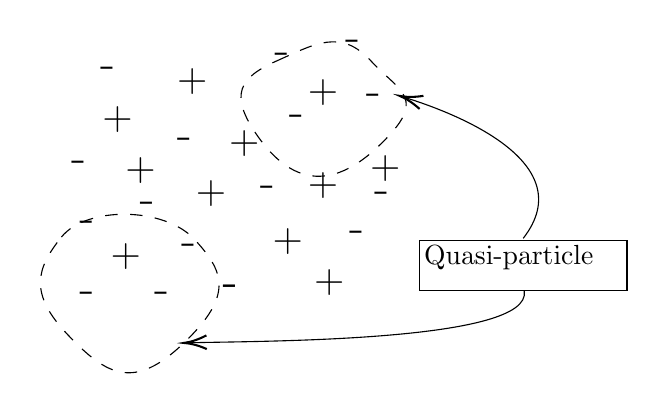
\begin{tikzpicture}[x=0.75pt,y=0.75pt,yscale=-1,xscale=1]
%uncomment if require: \path (0,300); %set diagram left start at 0, and has height of 300

%Shape: Polygon Curved [id:ds393267198766974] 
\draw  [dash pattern={on 4.5pt off 4.5pt}] (104.52,151.27) .. controls (116.52,136.27) and (154.03,136.65) .. (168.52,152.27) .. controls (183,167.88) and (187.52,179.27) .. (163.52,202.27) .. controls (139.52,225.27) and (126.52,218.27) .. (107.52,198.27) .. controls (88.52,178.27) and (92.52,166.27) .. (104.52,151.27) -- cycle ;
%Shape: Polygon Curved [id:ds5938648082047331] 
\draw  [dash pattern={on 4.5pt off 4.5pt}] (208.52,66.27) .. controls (226.52,58.27) and (239.03,50.65) .. (253.52,66.27) .. controls (268,81.88) and (281.52,84.27) .. (257.52,107.27) .. controls (233.52,130.27) and (214.52,124.27) .. (199.52,103.27) .. controls (184.52,82.27) and (190.52,74.27) .. (208.52,66.27) -- cycle ;
%Curve Lines [id:da7350178540870457] 
\draw    (327,151.88) .. controls (354.95,116) and (296.92,92.23) .. (269.18,83.77) ;
\draw [shift={(267.52,83.27)}, rotate = 376.5] [color={rgb, 255:red, 0; green, 0; blue, 0 }  ][line width=0.75]    (10.93,-3.29) .. controls (6.95,-1.4) and (3.31,-0.3) .. (0,0) .. controls (3.31,0.3) and (6.95,1.4) .. (10.93,3.29)   ;
%Curve Lines [id:da8754807282204362] 
\draw    (327.52,177.27) .. controls (331.46,201.89) and (200.54,201.29) .. (165.07,202.22) ;
\draw [shift={(163.52,202.27)}, rotate = 358.26] [color={rgb, 255:red, 0; green, 0; blue, 0 }  ][line width=0.75]    (10.93,-3.29) .. controls (6.95,-1.4) and (3.31,-0.3) .. (0,0) .. controls (3.31,0.3) and (6.95,1.4) .. (10.93,3.29)   ;

% Text Node
\draw (127,152.88) node [anchor=north west][inner sep=0.75pt]  [font=\Large] [align=left] {+};
% Text Node
\draw (141,128.88) node [anchor=north west][inner sep=0.75pt]  [font=\LARGE] [align=left] {\mbox{-}};
% Text Node
\draw (161,148.88) node [anchor=north west][inner sep=0.75pt]  [font=\LARGE] [align=left] {\mbox{-}};
% Text Node
\draw (148,171.88) node [anchor=north west][inner sep=0.75pt]  [font=\LARGE] [align=left] {\mbox{-}};
% Text Node
\draw (112,171.88) node [anchor=north west][inner sep=0.75pt]  [font=\LARGE] [align=left] {\mbox{-}};
% Text Node
\draw (112,137.88) node [anchor=north west][inner sep=0.75pt]  [font=\LARGE] [align=left] {\mbox{-}};
% Text Node
\draw (168,122.88) node [anchor=north west][inner sep=0.75pt]  [font=\Large] [align=left] {+};
% Text Node
\draw (205,145.88) node [anchor=north west][inner sep=0.75pt]  [font=\Large] [align=left] {+};
% Text Node
\draw (181,168.88) node [anchor=north west][inner sep=0.75pt]  [font=\LARGE] [align=left] {\mbox{-}};
% Text Node
\draw (181,168.88) node [anchor=north west][inner sep=0.75pt]  [font=\LARGE] [align=left] {\mbox{-}};
% Text Node
\draw (242,142.88) node [anchor=north west][inner sep=0.75pt]  [font=\LARGE] [align=left] {\mbox{-}};
% Text Node
\draw (199,120.88) node [anchor=north west][inner sep=0.75pt]  [font=\LARGE] [align=left] {\mbox{-}};
% Text Node
\draw (222,118.88) node [anchor=north west][inner sep=0.75pt]  [font=\Large] [align=left] {+};
% Text Node
\draw (184,98.88) node [anchor=north west][inner sep=0.75pt]  [font=\Large] [align=left] {+};
% Text Node
\draw (159,97.88) node [anchor=north west][inner sep=0.75pt]  [font=\LARGE] [align=left] {\mbox{-}};
% Text Node
\draw (254,123.88) node [anchor=north west][inner sep=0.75pt]  [font=\LARGE] [align=left] {\mbox{-}};
% Text Node
\draw (213,86.88) node [anchor=north west][inner sep=0.75pt]  [font=\LARGE] [align=left] {\mbox{-}};
% Text Node
\draw (250,76.88) node [anchor=north west][inner sep=0.75pt]  [font=\LARGE] [align=left] {\mbox{-}};
% Text Node
\draw (206,56.88) node [anchor=north west][inner sep=0.75pt]  [font=\LARGE] [align=left] {\mbox{-}};
% Text Node
\draw (240,50.88) node [anchor=north west][inner sep=0.75pt]  [font=\LARGE] [align=left] {\mbox{-}};
% Text Node
\draw (252,110.88) node [anchor=north west][inner sep=0.75pt]  [font=\Large] [align=left] {+};
% Text Node
\draw (222,73.88) node [anchor=north west][inner sep=0.75pt]  [font=\Large] [align=left] {+};
% Text Node
\draw (225,165.88) node [anchor=north west][inner sep=0.75pt]  [font=\Large] [align=left] {+};
% Text Node
\draw (159,68.88) node [anchor=north west][inner sep=0.75pt]  [font=\Large] [align=left] {+};
% Text Node
\draw (123,86.88) node [anchor=north west][inner sep=0.75pt]  [font=\Large] [align=left] {+};
% Text Node
\draw (108,108.88) node [anchor=north west][inner sep=0.75pt]  [font=\LARGE] [align=left] {\mbox{-}};
% Text Node
\draw (122,63.88) node [anchor=north west][inner sep=0.75pt]  [font=\LARGE] [align=left] {\mbox{-}};
% Text Node
\draw (134,111.88) node [anchor=north west][inner sep=0.75pt]  [font=\Large] [align=left] {+};
% Text Node
\draw    (277,152.88) -- (377,152.88) -- (377,176.88) -- (277,176.88) -- cycle  ;
\draw (278,153.88) node [anchor=north west][inner sep=0.75pt]   [align=left] {Quasi-particle};


\end{tikzpicture}

    \caption{Quasi particles in a Liquid of Positive and Negative Ions}
    \label{fig:quasi-particle-example}
\end{figure}
From Fig.\ref{fig:quasi-particle-example}, we know, from more powerful terminology of QFT:
\begin{center}
    "bare" particle + "clothing"/"cloud" = "dressed"/"renormalized" particle
\end{center}
For example, in quantum electrodynamics a 'bare' electron interacting with a field of photons acquires a cloud of virtual photons around it, converting it into the 'dressed' electron. In a similar manner, the interaction between real particles is called the 'bare' interaction, while the weak interaction between quasi particles is referred to as the 'effective' or "dressed" or "renormalized" interaction. \bluep{It should be noted that each bare particle is simultaneously the 'core' of a quasi particle and a transient 'member' of the cloud of several other quasi particles.}

The free quasi particles have a new energy law as 
$$\epsilon^{\prime}=\frac{p^{2}}{2 m^{*}} \quad \text { instead of } \quad \epsilon=\frac{p^{2}}{2 m}$$
where $m^*$ is the effective mass. The difference 
$$\epsilon_{quasi}-\epsilon_{bare}=\epsilon_{self}$$
is called \redp{\textbf{"self-energy"}} of the quasi particle.

@ Quantum System: quasi electreon in electron gas

The ' electron gas' is a simple model often used to describe many-body effects in metals. It consists of a box containing a large number of electrons interacting by means of the Coulomb force. In addition, there is a uniform, fixed, positive charge 'background' put into the box in order to keep the whole system electrically neutral. In the ground state, the electrons are spread out uniformly in the box.

Suppose now that we have a single, well-localized electron which we shoot into the electron gas  Because of the repulsive Coulomb interaction
between electrons, this extra electron repels other electrons away from it, so we get an empty space near the extra electron, and repelled electrons further away(Fig.\ref{fig:quasi-particle-example2}). This empty region may be viewed in a more detailed or microscopic way as composed of \redp{'holes'} in the electron gas. That is, the extra electron has "lifted out" electrons from the uniform charge distribution in its vicinity, thus creating 'holes' in this charge distribution, and has 'put down' these lifted-out electrons further away.
\begin{figure}[H]
    \centering
\tikzset {_0o14ioo3g/.code = {\pgfsetadditionalshadetransform{ \pgftransformshift{\pgfpoint{0 bp } { 0 bp }  }  \pgftransformscale{1 }  }}}
\pgfdeclareradialshading{_73ww2zakf}{\pgfpoint{0bp}{0bp}}{rgb(0bp)=(1,1,1);
rgb(12.019342694963727bp)=(1,1,1);
rgb(25bp)=(0,0,0);
rgb(400bp)=(0,0,0)}
\tikzset{_98ggw9slw/.code = {\pgfsetadditionalshadetransform{\pgftransformshift{\pgfpoint{0 bp } { 0 bp }  }  \pgftransformscale{1 } }}}
\pgfdeclareradialshading{_52d0oeat9} { \pgfpoint{0bp} {0bp}} {color(0bp)=(transparent!0);
color(12.019342694963727bp)=(transparent!0);
color(25bp)=(transparent!10);
color(400bp)=(transparent!10)} 
\pgfdeclarefading{_yzsmf2mqd}{\tikz \fill[shading=_52d0oeat9,_98ggw9slw] (0,0) rectangle (50bp,50bp); } 
\tikzset{every picture/.style={line width=0.75pt}} %set default line width to 0.75pt        

\begin{tikzpicture}[x=0.75pt,y=0.75pt,yscale=-1,xscale=1]
%uncomment if require: \path (0,300); %set diagram left start at 0, and has height of 300

%Shape: Rectangle [id:dp842398765103643] 
\draw  [fill={rgb, 255:red, 0; green, 0; blue, 0 }  ,fill opacity=1 ] (59.93,58.88) -- (235.32,58.88) -- (235.32,203.27) -- (59.93,203.27) -- cycle ;
%Shape: Circle [id:dp5878809314291961] 
\path  [shading=_73ww2zakf,_0o14ioo3g,path fading= _yzsmf2mqd ,fading transform={xshift=2}] (85.93,145.54) .. controls (85.93,131.37) and (97.42,119.88) .. (111.59,119.88) .. controls (125.76,119.88) and (137.25,131.37) .. (137.25,145.54) .. controls (137.25,159.71) and (125.76,171.2) .. (111.59,171.2) .. controls (97.42,171.2) and (85.93,159.71) .. (85.93,145.54) -- cycle ; % for fading 
 \draw   (85.93,145.54) .. controls (85.93,131.37) and (97.42,119.88) .. (111.59,119.88) .. controls (125.76,119.88) and (137.25,131.37) .. (137.25,145.54) .. controls (137.25,159.71) and (125.76,171.2) .. (111.59,171.2) .. controls (97.42,171.2) and (85.93,159.71) .. (85.93,145.54) -- cycle ; % for border 

%Shape: Circle [id:dp649192880176533] 
\draw  [fill={rgb, 255:red, 0; green, 0; blue, 0 }  ,fill opacity=1 ] (104.47,145.54) .. controls (104.47,141.61) and (107.66,138.42) .. (111.59,138.42) .. controls (115.53,138.42) and (118.72,141.61) .. (118.72,145.54) .. controls (118.72,149.48) and (115.53,152.67) .. (111.59,152.67) .. controls (107.66,152.67) and (104.47,149.48) .. (104.47,145.54) -- cycle ;
%Straight Lines [id:da47546531201986364] 
\draw [color={rgb, 255:red, 232; green, 30; blue, 12 }  ,draw opacity=1 ][line width=1.5]    (111.59,145.54) -- (135.11,122.37) ;
\draw [shift={(137.25,120.27)}, rotate = 495.43] [color={rgb, 255:red, 232; green, 30; blue, 12 }  ,draw opacity=1 ][line width=1.5]    (14.21,-4.28) .. controls (9.04,-1.82) and (4.3,-0.39) .. (0,0) .. controls (4.3,0.39) and (9.04,1.82) .. (14.21,4.28)   ;
%Shape: Rectangle [id:dp08609024153608191] 
\draw  [fill={rgb, 255:red, 0; green, 0; blue, 0 }  ,fill opacity=1 ] (261.93,58.88) -- (437.32,58.88) -- (437.32,203.27) -- (261.93,203.27) -- cycle ;
%Shape: Circle [id:dp8820237303823028] 
\draw  [fill={rgb, 255:red, 255; green, 255; blue, 255 }  ,fill opacity=1 ] (291,140.51) .. controls (291,136.3) and (294.41,132.88) .. (298.63,132.88) .. controls (302.84,132.88) and (306.25,136.3) .. (306.25,140.51) .. controls (306.25,144.72) and (302.84,148.13) .. (298.63,148.13) .. controls (294.41,148.13) and (291,144.72) .. (291,140.51) -- cycle ;
%Shape: Circle [id:dp5770389827427272] 
\draw  [fill={rgb, 255:red, 255; green, 255; blue, 255 }  ,fill opacity=1 ] (307,152.51) .. controls (307,148.3) and (310.41,144.88) .. (314.63,144.88) .. controls (318.84,144.88) and (322.25,148.3) .. (322.25,152.51) .. controls (322.25,156.72) and (318.84,160.13) .. (314.63,160.13) .. controls (310.41,160.13) and (307,156.72) .. (307,152.51) -- cycle ;
%Shape: Circle [id:dp025362450260817182] 
\draw  [fill={rgb, 255:red, 255; green, 255; blue, 255 }  ,fill opacity=1 ] (297,168.51) .. controls (297,164.3) and (300.41,160.88) .. (304.63,160.88) .. controls (308.84,160.88) and (312.25,164.3) .. (312.25,168.51) .. controls (312.25,172.72) and (308.84,176.13) .. (304.63,176.13) .. controls (300.41,176.13) and (297,172.72) .. (297,168.51) -- cycle ;
%Shape: Circle [id:dp9389847020012084] 
\draw  [fill={rgb, 255:red, 255; green, 255; blue, 255 }  ,fill opacity=1 ] (281,158.51) .. controls (281,154.3) and (284.41,150.88) .. (288.63,150.88) .. controls (292.84,150.88) and (296.25,154.3) .. (296.25,158.51) .. controls (296.25,162.72) and (292.84,166.13) .. (288.63,166.13) .. controls (284.41,166.13) and (281,162.72) .. (281,158.51) -- cycle ;
%Straight Lines [id:da4209538731972077] 
\draw [color={rgb, 255:red, 232; green, 30; blue, 12 }  ,draw opacity=1 ][line width=1.5]    (298.63,140.51) -- (293.85,117.21) ;
\draw [shift={(293.25,114.27)}, rotate = 438.42] [color={rgb, 255:red, 232; green, 30; blue, 12 }  ,draw opacity=1 ][line width=1.5]    (14.21,-4.28) .. controls (9.04,-1.82) and (4.3,-0.39) .. (0,0) .. controls (4.3,0.39) and (9.04,1.82) .. (14.21,4.28)   ;
%Straight Lines [id:da6368743975733171] 
\draw [color={rgb, 255:red, 232; green, 30; blue, 12 }  ,draw opacity=1 ][line width=1.5]    (314.63,152.51) -- (338.31,147.85) ;
\draw [shift={(341.25,147.27)}, rotate = 528.86] [color={rgb, 255:red, 232; green, 30; blue, 12 }  ,draw opacity=1 ][line width=1.5]    (14.21,-4.28) .. controls (9.04,-1.82) and (4.3,-0.39) .. (0,0) .. controls (4.3,0.39) and (9.04,1.82) .. (14.21,4.28)   ;
%Straight Lines [id:da3789740110796589] 
\draw [color={rgb, 255:red, 232; green, 30; blue, 12 }  ,draw opacity=1 ][line width=1.5]    (304.63,168.51) -- (322.7,179.69) ;
\draw [shift={(325.25,181.27)}, rotate = 211.74] [color={rgb, 255:red, 232; green, 30; blue, 12 }  ,draw opacity=1 ][line width=1.5]    (14.21,-4.28) .. controls (9.04,-1.82) and (4.3,-0.39) .. (0,0) .. controls (4.3,0.39) and (9.04,1.82) .. (14.21,4.28)   ;
%Straight Lines [id:da1630717526737726] 
\draw [color={rgb, 255:red, 232; green, 30; blue, 12 }  ,draw opacity=1 ][line width=1.5]    (288.63,158.51) -- (272.53,172.31) ;
\draw [shift={(270.25,174.27)}, rotate = 319.38] [color={rgb, 255:red, 232; green, 30; blue, 12 }  ,draw opacity=1 ][line width=1.5]    (14.21,-4.28) .. controls (9.04,-1.82) and (4.3,-0.39) .. (0,0) .. controls (4.3,0.39) and (9.04,1.82) .. (14.21,4.28)   ;

% Text Node
\draw (256,212.88) node [anchor=north west][inner sep=0.75pt]  [font=\footnotesize] [align=left] {(b)Lifted-out electrons create "holes"};
% Text Node
\draw (36,212.88) node [anchor=north west][inner sep=0.75pt]  [font=\footnotesize] [align=left] {(a)"Empty" region near the electron};


\end{tikzpicture}
    \caption{Extra Electron Pushes Other Electrons Away}
    \label{fig:quasi-particle-example2}
\end{figure}

@ Bogoliubov quasi particles ("bogolons")

These are the elementary excitations in a superconductor. We include them here since they are called quasi particles, but actually their structure is quite different from the 'particle plus cloud' picture described above. They consist of a linear combination ofan electron in state $(+k, \uparrow)$ and a hole $^{\prime}$ in $(-k, \downarrow)$.

\end{easylist}

\subsection{A Brief Intro to Collective Excitations}
As we have seen, the quasi particle consists of the original real, individual particle, plus a cloud of disturbed neighbours. It behaves very much like an
individual particle, except that it has an effective mass and a lifetime. But there also exist other kinds of fictitious particles in many-body systems, i.e., 'collective excitations'. These do not centre around individual particles, but instead involve collective, wavelike motion of all the particles in the system
simultaneously. Here are some examples:
\begin{easylist}
\NewList
@ Plasmons

If a thin metal foil is bombarded with high energy electrons, it is possible to set up sinusoidal oscillations in the density of the electron gas in the foil. This is known as a \bluep{'plasma wave'}, and it has a frequency $\omega_p$ and wavelength $\lambda_p$. \bluep{The plasma wave may be visualized as built up of 'holes' in the low-density regions and extra electrons in the high-density regions}. Just as light waves are quantized into units having energy $E=\hbar \omega$ called photons, plasma waves are quantized into units with energy $E_{p}=\hbar \omega_{p}$ called plasmons.

@ phonons

Sound waves are sinusoidal oscillations in the crystal lattice ofa solid. They are quantized into collective excitations called 'phonons'.

@ Magnons

In ferromagnets there are regular fluctuations in the density of spin angular momentum known as spin waves. The collective excitation here is the spin
wave quantum known as the 'magnon".
\end{easylist}

\subsection{Propagators-the Keys to the Many-body Problem}
The idea behind the propagator method is this: the detailed description of a many-body system requires in the classical case the position of each particle as a function of time, or in the quantum case, the time dependent wave function of the whole system. Fortunately, it turns out that \textbf{in order to find the important physical properties of a system it is not necessary to know the detailed behaviour of each particle in the system, but rather just the average behaviour of one or two typical particles.} \bluep{The quantities which describe this average behaviour are the\textit{ one-particle propagator} and \textit{two-particle propagator} respectively, and physical properties may be calculated directly from them.}

\begin{imp}
\textbf{One-particle propagator}: we put a particle into the interacting system at point $r_{1}$ at time $t_{1}$ and let it move through the system colliding with the other particles for a while (i.e., let it "propagate" through the system). Then the one-particle propagator is the probability (or in quantum systems, the probability amplitude) that the particle will be observed at the point $r_{2}$ at time $t_{2} .$ (Note that instead of putting the particle in at a definite point, it is sometimes more convenient to put it in with definite momentum, say $p_{1},$ and observe it later with momentum $p_{2} .$ ) \bluep{The single-particle propagator yields directly the energies and lifetimes of quasi particles. It also gives the momentum distribution, spin and particle density and can be used to calculate the ground state energy.}
\end{imp}
\begin{imp}
\textbf{Two-particle propagator}: the probability amplitude for observing one particle at $r_{2}, t_{2}$ and another at $r_{4}, t_{4}$ if one was put into the system at $r_{1}, t_{1}$ and another at $r_{3}, t_{3}$. This also has a wide variety of talents, \bluep{giving directly the energies and lifetimes of collective excitations, as well as the magnetic susceptibility, electrical conductivity, and a host of other non-cquilibrium properties.}
\end{imp}

\subsection{Calculate Propagator:the drunk man example}
With the aid of Feynman diagrams, we expand the propagator in an infinite series and evaluate the series approximately. This can be carried out in a general, systematic, and picturesque way.

Just to get an idea of what these diagrams are, consider the following simple example. A man who has had too much to drink, leaves a party at point 1 and on the way to his home at point 2, he can stop off at one or more bars-Alice's Bar (A), Bardot Bar (B), Club Six Bar (C), ... , etc. He can wind up either at his own home 2, or at any one of his friends' apartments, 3, 4, etc. We ask for the probability, P(2, I), that he gets home. This probability, which is just the propagator here (with time omitted for simplicity), is the sum of the probabilities for all the different ways he can propagate from I to 2 interacting with the various bars.

The first way he can prophgate is ' freely' from 1 to 2, i.e., without stopping at a bar. Call the probability for this free propagation $P_{0}(2,1)$

The second way he can propagate is to go freely from 1 to bar $A$ (the probability for this is $P_{0}(A, 1)$ ), then stop off at bar $A$ for a drink (call the probability for this $P(A))$, then go freely from $A$ to 2 (probability $=P_{0}(2, A)$ ). Assume for simplicity that the three processes here are independent. Then the total probability for this second way is the product of the probabilities for each process taken separately, i.e., $P_{0}(A, 1) \times P(A) \times P_{0}(2, A) .$ (This is like the case in coin-tossing: since each toss is independent, the probability of first tossing a head, then a tail, equals the probability of tossing a head times the probability of tossing a tail.)

The third way he can propagate is from 1 to $B$ to $2,$ with probability $P_{0}(B, 1) P(B) P_{0}(2, B) .$ Or he could go from 1 to $C$ to $2,$ etc., or from 1 to $A$ to $B$ to $2,$ or from 1 to $A,$ come out of $A,$ go back into $A,$ then go to $2,$ and so on. The total probability, $P(2,1)$ is then given by the sum of the probabilities for each way, i.e., the infinite series:
$$\begin{aligned}
P(2,1)=&P_{0}(2,1)+P_{0}(A, 1) P(A) P_{0}(2, A)+P_{0}(B, 1) P(B) P_{0}(2, B)+\cdots  \\
&+P_{0}(A, 1) P(A) P_{0}(B, A) P(B) P_{0}(2, B)+\cdots
\end{aligned}$$
\redp{This is an example of a 'perturbation series', since each interaction with a bar "perturbs" the free propagation of the drunken man.} Represent this series using the following dictionary:
\begin{figure}[H]
    \centering
\tikzset{every picture/.style={line width=0.75pt}} %set default line width to 0.75pt        

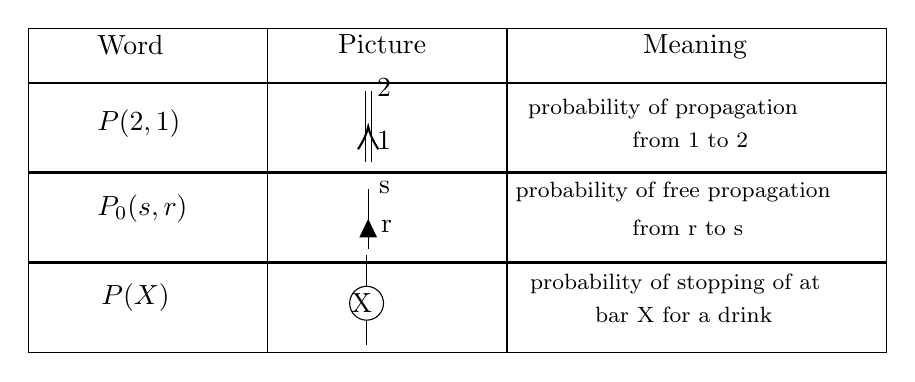
\begin{tikzpicture}[x=0.75pt,y=0.75pt,yscale=-1,xscale=1]
%uncomment if require: \path (0,349); %set diagram left start at 0, and has height of 349

%Shape: Rectangle [id:dp3972753239553969] 
\draw   (212.78,159.32) -- (328.11,159.32) -- (328.11,185.7) -- (212.78,185.7) -- cycle ;
%Shape: Rectangle [id:dp013530620031451002] 
\draw   (328.11,159.32) -- (443.44,159.32) -- (443.44,185.7) -- (328.11,185.7) -- cycle ;
%Shape: Rectangle [id:dp736076383888415] 
\draw   (443.44,159.32) -- (626.17,159.32) -- (626.17,185.7) -- (443.44,185.7) -- cycle ;
%Shape: Rectangle [id:dp018483080609867475] 
\draw   (212.78,185.32) -- (328.11,185.32) -- (328.11,229.2) -- (212.78,229.2) -- cycle ;
%Shape: Rectangle [id:dp18336509171990412] 
\draw   (328.11,185.32) -- (443.44,185.32) -- (443.44,229.2) -- (328.11,229.2) -- cycle ;
%Shape: Rectangle [id:dp5452879627568872] 
\draw   (443.44,185.32) -- (626.17,185.32) -- (626.17,229.2) -- (443.44,229.2) -- cycle ;
%Shape: Rectangle [id:dp710141061414926] 
\draw   (212.78,228.57) -- (328.11,228.57) -- (328.11,272.45) -- (212.78,272.45) -- cycle ;
%Shape: Rectangle [id:dp6981715844716105] 
\draw   (328.11,228.57) -- (443.44,228.57) -- (443.44,272.45) -- (328.11,272.45) -- cycle ;
%Shape: Rectangle [id:dp9707206740138988] 
\draw   (443.44,228.57) -- (626.17,228.57) -- (626.17,272.45) -- (443.44,272.45) -- cycle ;
%Shape: Rectangle [id:dp7188406169431831] 
\draw   (212.78,271.81) -- (328.11,271.81) -- (328.11,315.7) -- (212.78,315.7) -- cycle ;
%Shape: Rectangle [id:dp35373677352561617] 
\draw   (328.11,271.81) -- (443.44,271.81) -- (443.44,315.7) -- (328.11,315.7) -- cycle ;
%Shape: Rectangle [id:dp7761518007990666] 
\draw   (443.44,271.81) -- (626.17,271.81) -- (626.17,315.7) -- (443.44,315.7) -- cycle ;
%Straight Lines [id:da3953067075421305] 
\draw    (375.07,223.7) -- (375.07,189.7)(378.07,223.7) -- (378.07,189.7) ;
\draw [shift={(376.57,206.7)}, rotate = 450] [color={rgb, 255:red, 0; green, 0; blue, 0 }  ][line width=0.75]    (10.93,-4.9) .. controls (6.95,-2.3) and (3.31,-0.67) .. (0,0) .. controls (3.31,0.67) and (6.95,2.3) .. (10.93,4.9)   ;
%Straight Lines [id:da5701847229817978] 
\draw    (376.57,265.7) -- (376.57,236.7) ;
\draw [shift={(376.57,251.2)}, rotate = 450] [fill={rgb, 255:red, 0; green, 0; blue, 0 }  ][line width=0.08]  [draw opacity=0] (8.93,-4.29) -- (0,0) -- (8.93,4.29) -- cycle    ;
%Shape: Ellipse [id:dp16063069982491784] 
\draw   (367.64,291.82) .. controls (367.64,287.31) and (371.29,283.66) .. (375.79,283.66) .. controls (380.3,283.66) and (383.95,287.31) .. (383.95,291.82) .. controls (383.95,296.32) and (380.3,299.97) .. (375.79,299.97) .. controls (371.29,299.97) and (367.64,296.32) .. (367.64,291.82) -- cycle ;
%Straight Lines [id:da2549697012881261] 
\draw    (375.79,283.66) -- (375.79,268.7) ;
%Straight Lines [id:da05824951890975272] 
\draw    (375.79,311.7) -- (375.79,299.97) ;

% Text Node
\draw (244.78,161.32) node [anchor=north west][inner sep=0.75pt]   [align=left] {Word};
% Text Node
\draw (360.78,161.32) node [anchor=north west][inner sep=0.75pt]   [align=left] {Picture};
% Text Node
\draw (507.78,161.32) node [anchor=north west][inner sep=0.75pt]   [align=left] {Meaning};
% Text Node
\draw (244.78,197.32) node [anchor=north west][inner sep=0.75pt]    {$P( 2,1)$};
% Text Node
\draw (379.57,207.76) node [anchor=north west][inner sep=0.75pt]   [align=left] {1};
% Text Node
\draw (379.57,182.54) node [anchor=north west][inner sep=0.75pt]   [align=left] {2};
% Text Node
\draw (244.78,238.32) node [anchor=north west][inner sep=0.75pt]    {$P_{0}( s,r)$};
% Text Node
\draw (381.57,250.76) node [anchor=north west][inner sep=0.75pt]   [align=left] {r};
% Text Node
\draw (380.57,231.7) node [anchor=north west][inner sep=0.75pt]   [align=left] {s};
% Text Node
\draw (367.2,285.75) node [anchor=north west][inner sep=0.75pt]   [align=left] {X};
% Text Node
\draw (246.78,281.32) node [anchor=north west][inner sep=0.75pt]    {$P( X)$};
% Text Node
\draw (452.33,192.32) node [anchor=north west][inner sep=0.75pt]  [font=\footnotesize] [align=left] {probability of propagation };
% Text Node
\draw (502.63,208.32) node [anchor=north west][inner sep=0.75pt]  [font=\footnotesize] [align=left] {from 1 to 2};
% Text Node
\draw (446.33,232.32) node [anchor=north west][inner sep=0.75pt]  [font=\footnotesize] [align=left] {probability of free propagation };
% Text Node
\draw (502.63,250.32) node [anchor=north west][inner sep=0.75pt]  [font=\footnotesize] [align=left] {from r to s};
% Text Node
\draw (453.33,276.32) node [anchor=north west][inner sep=0.75pt]  [font=\footnotesize] [align=left] {probability of stopping of at \ };
% Text Node
\draw (484.63,292.32) node [anchor=north west][inner sep=0.75pt]  [font=\footnotesize] [align=left] {bar X for a drink};


\end{tikzpicture}

    \caption{Diagram dictionary for drunken man}
    \label{fig:drunken-man-1}
\end{figure}
The perturbation series in diagrams for this drunken man propagator is therefore
\begin{figure}[H]
    \centering
    


\tikzset{every picture/.style={line width=0.75pt}} %set default line width to 0.75pt        

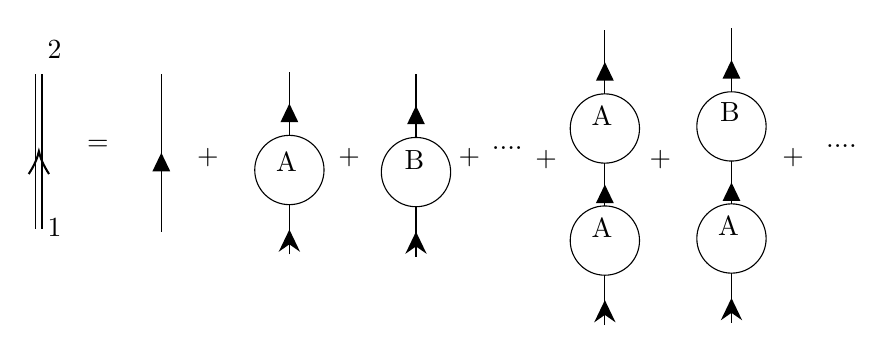
\begin{tikzpicture}[x=0.75pt,y=0.75pt,yscale=-1,xscale=1]
%uncomment if require: \path (0,349); %set diagram left start at 0, and has height of 349

%Straight Lines [id:da4757935872975344] 
\draw    (8.07,101.32) -- (8.07,26.7)(11.07,101.32) -- (11.07,26.7) ;
\draw [shift={(9.57,64.01)}, rotate = 450] [color={rgb, 255:red, 0; green, 0; blue, 0 }  ][line width=0.75]    (10.93,-4.9) .. controls (6.95,-2.3) and (3.31,-0.67) .. (0,0) .. controls (3.31,0.67) and (6.95,2.3) .. (10.93,4.9)   ;
%Straight Lines [id:da23622371172830803] 
\draw    (68.57,102.7) -- (68.57,26.7) ;
\draw [shift={(68.57,64.7)}, rotate = 450] [fill={rgb, 255:red, 0; green, 0; blue, 0 }  ][line width=0.08]  [draw opacity=0] (8.93,-4.29) -- (0,0) -- (8.93,4.29) -- cycle    ;
%Shape: Circle [id:dp4139523862436749] 
\draw   (113.57,73.01) .. controls (113.57,63.79) and (121.04,56.32) .. (130.26,56.32) .. controls (139.48,56.32) and (146.95,63.79) .. (146.95,73.01) .. controls (146.95,82.23) and (139.48,89.7) .. (130.26,89.7) .. controls (121.04,89.7) and (113.57,82.23) .. (113.57,73.01) -- cycle ;
%Straight Lines [id:da33169967910609544] 
\draw    (130.26,56.32) -- (130.26,25.7) ;
\draw [shift={(130.26,41.01)}, rotate = 450] [fill={rgb, 255:red, 0; green, 0; blue, 0 }  ][line width=0.08]  [draw opacity=0] (8.93,-4.29) -- (0,0) -- (8.93,4.29) -- cycle    ;
%Straight Lines [id:da28347419222198567] 
\draw    (130.26,113.7) -- (130.26,89.7) ;
\draw [shift={(130.26,101.7)}, rotate = 450] [fill={rgb, 255:red, 0; green, 0; blue, 0 }  ][line width=0.08]  [draw opacity=0] (10.72,-5.15) -- (0,0) -- (10.72,5.15) -- (7.12,0) -- cycle    ;
%Shape: Circle [id:dp1723289826034129] 
\draw   (174.57,74.01) .. controls (174.57,64.79) and (182.04,57.32) .. (191.26,57.32) .. controls (200.48,57.32) and (207.95,64.79) .. (207.95,74.01) .. controls (207.95,83.23) and (200.48,90.7) .. (191.26,90.7) .. controls (182.04,90.7) and (174.57,83.23) .. (174.57,74.01) -- cycle ;
%Straight Lines [id:da40381754331686626] 
\draw    (191.26,57.32) -- (191.26,26.7) ;
\draw [shift={(191.26,42.01)}, rotate = 450] [fill={rgb, 255:red, 0; green, 0; blue, 0 }  ][line width=0.08]  [draw opacity=0] (8.93,-4.29) -- (0,0) -- (8.93,4.29) -- cycle    ;
%Straight Lines [id:da5172106067784763] 
\draw    (191.26,114.7) -- (191.26,90.7) ;
\draw [shift={(191.26,102.7)}, rotate = 450] [fill={rgb, 255:red, 0; green, 0; blue, 0 }  ][line width=0.08]  [draw opacity=0] (10.72,-5.15) -- (0,0) -- (10.72,5.15) -- (7.12,0) -- cycle    ;
%Shape: Circle [id:dp663325870350397] 
\draw   (265.57,107.01) .. controls (265.57,97.79) and (273.04,90.32) .. (282.26,90.32) .. controls (291.48,90.32) and (298.95,97.79) .. (298.95,107.01) .. controls (298.95,116.23) and (291.48,123.7) .. (282.26,123.7) .. controls (273.04,123.7) and (265.57,116.23) .. (265.57,107.01) -- cycle ;
%Straight Lines [id:da6913773132395338] 
\draw    (282.26,36.32) -- (282.26,5.7) ;
\draw [shift={(282.26,21.01)}, rotate = 450] [fill={rgb, 255:red, 0; green, 0; blue, 0 }  ][line width=0.08]  [draw opacity=0] (8.93,-4.29) -- (0,0) -- (8.93,4.29) -- cycle    ;
%Straight Lines [id:da4724377841227787] 
\draw    (282.26,147.7) -- (282.26,123.7) ;
\draw [shift={(282.26,135.7)}, rotate = 450] [fill={rgb, 255:red, 0; green, 0; blue, 0 }  ][line width=0.08]  [draw opacity=0] (10.72,-5.15) -- (0,0) -- (10.72,5.15) -- (7.12,0) -- cycle    ;
%Shape: Circle [id:dp29262051024858293] 
\draw   (265.57,53.01) .. controls (265.57,43.79) and (273.04,36.32) .. (282.26,36.32) .. controls (291.48,36.32) and (298.95,43.79) .. (298.95,53.01) .. controls (298.95,62.23) and (291.48,69.7) .. (282.26,69.7) .. controls (273.04,69.7) and (265.57,62.23) .. (265.57,53.01) -- cycle ;
%Straight Lines [id:da2293551017015375] 
\draw    (282.26,69.7) -- (282.26,90.32) ;
\draw [shift={(282.26,80.01)}, rotate = 90] [fill={rgb, 255:red, 0; green, 0; blue, 0 }  ][line width=0.08]  [draw opacity=0] (8.93,-4.29) -- (0,0) -- (8.93,4.29) -- cycle    ;
%Shape: Circle [id:dp5742274191772756] 
\draw   (326.57,106.01) .. controls (326.57,96.79) and (334.04,89.32) .. (343.26,89.32) .. controls (352.48,89.32) and (359.95,96.79) .. (359.95,106.01) .. controls (359.95,115.23) and (352.48,122.7) .. (343.26,122.7) .. controls (334.04,122.7) and (326.57,115.23) .. (326.57,106.01) -- cycle ;
%Straight Lines [id:da8337372469854066] 
\draw    (343.26,35.32) -- (343.26,4.7) ;
\draw [shift={(343.26,20.01)}, rotate = 450] [fill={rgb, 255:red, 0; green, 0; blue, 0 }  ][line width=0.08]  [draw opacity=0] (8.93,-4.29) -- (0,0) -- (8.93,4.29) -- cycle    ;
%Straight Lines [id:da42712440571211296] 
\draw    (343.26,146.7) -- (343.26,122.7) ;
\draw [shift={(343.26,134.7)}, rotate = 450] [fill={rgb, 255:red, 0; green, 0; blue, 0 }  ][line width=0.08]  [draw opacity=0] (10.72,-5.15) -- (0,0) -- (10.72,5.15) -- (7.12,0) -- cycle    ;
%Shape: Circle [id:dp5287893719741432] 
\draw   (326.57,52.01) .. controls (326.57,42.79) and (334.04,35.32) .. (343.26,35.32) .. controls (352.48,35.32) and (359.95,42.79) .. (359.95,52.01) .. controls (359.95,61.23) and (352.48,68.7) .. (343.26,68.7) .. controls (334.04,68.7) and (326.57,61.23) .. (326.57,52.01) -- cycle ;
%Straight Lines [id:da8377025286119076] 
\draw    (343.26,68.7) -- (343.26,89.32) ;
\draw [shift={(343.26,79.01)}, rotate = 90] [fill={rgb, 255:red, 0; green, 0; blue, 0 }  ][line width=0.08]  [draw opacity=0] (8.93,-4.29) -- (0,0) -- (8.93,4.29) -- cycle    ;

% Text Node
\draw (12.57,95.32) node [anchor=north west][inner sep=0.75pt]   [align=left] {1};
% Text Node
\draw (12.57,9.32) node [anchor=north west][inner sep=0.75pt]   [align=left] {2};
% Text Node
\draw (31.57,57.32) node [anchor=north west][inner sep=0.75pt]   [align=left] {=};
% Text Node
\draw (122.57,63.32) node [anchor=north west][inner sep=0.75pt]   [align=left] {A};
% Text Node
\draw (184.57,62.32) node [anchor=north west][inner sep=0.75pt]   [align=left] {B};
% Text Node
\draw (336.57,39.32) node [anchor=north west][inner sep=0.75pt]   [align=left] {B};
% Text Node
\draw (335.57,94.32) node [anchor=north west][inner sep=0.75pt]   [align=left] {A};
% Text Node
\draw (274.57,95.32) node [anchor=north west][inner sep=0.75pt]   [align=left] {A};
% Text Node
\draw (274.57,41.32) node [anchor=north west][inner sep=0.75pt]   [align=left] {A};
% Text Node
\draw (84.57,61.32) node [anchor=north west][inner sep=0.75pt]    {$+$};
% Text Node
\draw (152.57,61.32) node [anchor=north west][inner sep=0.75pt]    {$+$};
% Text Node
\draw (210.57,61.32) node [anchor=north west][inner sep=0.75pt]    {$+$};
% Text Node
\draw (226.57,60.32) node [anchor=north west][inner sep=0.75pt]   [align=left] {....};
% Text Node
\draw (247.57,62.32) node [anchor=north west][inner sep=0.75pt]    {$+$};
% Text Node
\draw (302.57,62.32) node [anchor=north west][inner sep=0.75pt]    {$+$};
% Text Node
\draw (366.57,61.32) node [anchor=north west][inner sep=0.75pt]    {$+$};
% Text Node
\draw (387.57,59.32) node [anchor=north west][inner sep=0.75pt]   [align=left] {....};


\end{tikzpicture}

    \caption{Drunken man series}
    \label{fig:drunken-man-2}
\end{figure}

\subsection{Single-particle propagator for system of many interacting particles}

\subsection{The two-particle propagator and the particle-hole propagator}
\newpage
\section{Quantum Quasi Particles and the Quantum Pinball Propagator}
In the quantum case, the total probability amplitude is the sum of the probability amplitudes for each process taken separately
$$G(2,1)=G(\text { process } 1)+G(\text { process } 11)+\cdots$$
so that the corresponding probability is given by
$$P(2,1)_{\text {quantum }}=G^{*} G=\underbrace{|G(\mathrm{I})|^{2}}_{P(\mathrm{I})}+\underbrace{|G(\mathrm{I})|^{2}}_{P(\mathrm{II})}+\underbrace{G(\mathrm{I})^{*} G(\mathrm{II})+G(\mathrm{II})^{*} G(\mathrm{I})}_{\text {interference terms }}+\cdots$$
Because of the characteristic interference terms', the quantum probability is not just the sum of the probabilities for the individual processes, in contrast to the classical case.

Let us begin by defining the quantum propagator in general, then show
what it looks like in the case of free particles and quasi particles. The quantum analogue of the classical propagator is (assuming that the Hamiltonian is time-independent, so that the propagator depends only on time differences):
\begin{imp}
\begin{equation}i G\left(\mathrm{r}_{2}, \mathrm{r}_{1}, t_{2}-t_{1}\right)_{t_{2}>t_{1}}=i G^{+}\left(\mathrm{x}_{2}, \mathrm{r}_{1}, t_{2}-t_{1}\right)\end{equation}
probability amplitude that if at time $t_{1}$ we add a particle at point $r_{1}$ to the interacting system in its ground state, then at time $t_{2}$ the system will be in its ground state with an added particle at $\mathbf{r}_{2}$
\end{imp}
The $i$ factor is purely for decoration (a matter of convention) and the $+$ superscript denotes $t_{2}>t_{1} .$ The probability corresponding to the amplitude is
$$P\left(\mathbf{r}_{2}, \mathbf{r}_{1}, t_{2}-t_{1}\right)=G^{+}\left(r_{2}, \mathbf{r}_{1}, t_{2}-t_{1}\right)^{*} G^{+}\left(\mathbf{r}_{2}, \mathbf{r}_{1}, t_{2}-t_{1}\right)$$
Note that it is not necessarily the 'same' particle which is observed at 12, since
this has no meaning in the systems of identical particles with which we shall generally deal. The quantity $G^{+}$ is called a \bluep{'retarded' propagator (or Green's function)}. By definition, it is equal to zero for $t_{2} \leqslant t_{1} .$ There is also an \bluep{'advanced' propagator, $G^{-},$ which is finite for $t_{2} \leqslant t_{1} $}.

It is actually more convenient to work with an equivalent definition of $G$ in terms of arbitrary single-particle eigenstates, $\phi_{k}(r),$ instead of position eigenstates. Then we have \redp{$i G^{+}\left(k_{2}, k_{1}, t_{2}-t_{1}\right)_{t_{2}>t_{1}}=$probability amplitude that if at time $t_{1}$ we add a particle in $\phi_{k_{1}}(r)$ to the interacting system in its ground state, then at time $t_{2}$ the system will be in its ground state with an added particle in $\phi_{k_{2}}(r)$}.
For $t_{2} \leqslant t_{1}, G^{+}$ is defined so that:
\begin{equation}i G^{+}\left(k_{2}, k_{1}, t_{2}-t_{1}\right)_{t_{2}\leq t_{1}}=0\end{equation}
\textbf{A convenient choice for $\phi_{k}(r)$ is the eigenstates of the unperturbed single particle Hamiltonian, which we will call $H_{0}$ :}
$$H_{0}=\frac{p^{2}}{2 m}+U(\mathrm{r})=-\frac{1}{2 m} \nabla_{r}^{2}+U(\mathrm{r}) \quad(\hbar=1)$$
If $U(\mathrm{r})=0,$ then this is just the free particle case:
$$H_{0} \phi_{k}(\mathbf{r})=\epsilon_{k} \phi_{k}(\mathbf{r})$$
and
\begin{equation}H_{0}=-\frac{\nabla_{r}^{2}}{2 m}, \quad \phi_{k}(r)=\frac{1}{\sqrt{\Omega}} e^{i k \cdot r}, \quad \epsilon_{k}=\frac{k^{2}}{2 m}
\label{nrqm-free-particle}
\end{equation}
where $\Omega$ is normalization volume and spin is neglected for simplicity. Note that if $k_1=k_2$, the particle propagates in time only.

Let us first get the free propagator $G_{0}^{+}$ (no perturbing interaction). Suppose at time $t_{1}$ the wave function of the free particle is $\phi_{k,}(\mathrm{r}) .$ Then we have:
$$\psi\left(\mathbf{r}, t_{1}\right)=\phi_{\mathbf{k}_{2}}(\mathbf{r})$$
At later time $t_{2},$ by the time-dependent Schrödinger equation, we find that the wave function has become
\begin{equation}\psi\left(\mathbf{r}, t_{2}\right)=\phi_{k_{1}}(\mathbf{r}) e^{-i \varepsilon_{k1}\left(t_{2}-t_{1}\right)}
\end{equation}
where $\epsilon_{k_{1}}$ is the single particle energy of undisturbed Shrodinger equation. The probability amplitude for the particle being in state $\phi_{k_{2}}$ at time $t_{2}$ is /hen just the component of $\psi\left(\mathbf{r}, t_{2}\right)$ along $\phi_{k_{2}}$ or:
\begin{equation}\int d^{3} \mathbf{r} \psi\left(\mathbf{r}, t_{2}\right) \phi_{k_{2}}^{*}(\mathbf{r})=e^{-i \exp \left(l_{2}-t_{1}\right)} \int \underbrace{d^{3} \mathbf{r} \phi_{k_{1}}(\mathbf{r}) \phi_{k_{2}}^{*}(\mathbf{r})}_{\delta_{k_{2} k_{1}}}\end{equation}
whence, by definition
\begin{equation}G_{0}^{+}\left(k, t_{2}-t_{1}\right)=\left\{\begin{array}{ll}
-i \theta_{12-t_{1}} e^{-i \epsilon_{k_1}\left(t_{2}-t_{1}\right)}, & \text { for } t_{2} \neq t_{1} \\
0, & \text { for } t_{2}=t_{1}
\end{array}\right.
\label{G0-+}
\end{equation}
where
$$\theta_{t_{2}-t_{1}}\left\{\begin{array}{ll}
=1, & \text { if } t_{2}>t_{1} \\
=0, & \text { if } t_{2}<t_{1}
\end{array}\right.$$
\bluep{Note that for fermions, all levles up to $\epsilon_F$(=Fermi energy) are fileed, so we can only propagate a particle with $\epsilon_{k_1}>\epsilon_F$}. The Fourier transform of (\ref{G0-+}) is
\begin{equation}\begin{aligned}
G_{0}^{+}(k, \omega) &=-i \int_{-\infty}^{+\infty} d\left(t_{2}-t_{1}\right) \theta_{t_{2}-t_{1}} e^{i \omega\left(t_{2}-t_{1}\right)} e^{-i \epsilon_{k}\left(t_{2}-t_{1}\right)} \\
&=\left.(-1) \frac{e^{i\left(\omega-\epsilon_{k}\right)\left(t_{2}-t_{1}\right)}}{\omega-\epsilon_{k}}\right|_{0} ^{\infty}=\frac{1}{\omega-\epsilon_{k}}-\frac{e^{i\left(\omega-\epsilon_{k}\right)\infty}}{\omega-\epsilon_{k}}
\end{aligned}
\label{G0-k-omega}
\end{equation}
\redp{Because of the exponential oscillating at $\infty,$ this function is not well defined. In order to get around this difficulty, we have to slightly modify the expression for the free propagator. This is done by multiplying the propagator by the factor $\exp \left(-\delta\left(t_{2}-t_{1}\right)\right),$ where $\delta$ is a positive infinitesimal such that $\delta \times \infty=\infty$}. Then (\ref{G0-+}) becomes:
\begin{equation}G_{0}^{+}\left(k, t_{2}-t_{1}\right)=-i \theta_{t_{2}-t_{1}}e^{i(\epsilon_k-i\delta)(t_2-t_1)}
\label{G0-with-delta}
\end{equation}
For any finite $\left(t_{2}-t_{1}\right),$ we have $\delta \times\left(t_{2}-t_{1}\right)=0,$ so this is just $(3.10) .$ But for infinite $\left(t_{2}-t_{1}\right), \delta \times\left(t_{2}-t_{1}\right)=\infty$ so $G_{0}^{+}=0 .$ When \ref{G0-with-delta} is placed in \ref{G0-k-omega} we find
\begin{imp}
\begin{equation}G_{o}^{+}(k, \omega)=\frac{1}{\omega-\epsilon_{k}+i \delta}
\label{G0-k-omega-delta}
\end{equation}
\end{imp}
\bluep{From \ref{G0-k-omega-delta} we see the pole is at $\omega=\epsilon_k$, the eigenvalue for the eigenstate $\phi_k$. It turns out this observation is quite general, even for interacting propagator, $G^+(k,l;\omega)$:}
\begin{imp}
The poles of $G^+(k,l,\omega),$ the fourier transform of the single-particle propagator, corresponds to the excited energy of (N+1)-particle system \textbf{minus the ground state energy of N-particle system}.
\end{imp}
Also from \ref{G0-k-omega-delta}, we have the particle lifetime $\tau$ as $\delta^{-1}=\infty$, which makes sense because we only consider one free particle here. This observation can also be extended to interacting system where the propagator has the form of 
\begin{equation}
    G^+=\frac{1}{\omega-\epsilon_k^{\prime}+i\tau_k^{-1}}
\end{equation}
where \redp{$\tau_k$ is the quasi-particle lifetime at the state of $\epsilon_k$}.

In a Fermi system, because of the Pauli's principle, each state can only be occupied by one fermion. If a state is partially occupied by a fermion, the possibility of adding another fermion at the same state will be less than 1. Hence we have to multiply the propagator by a factor $Z_k\leq 1$:
\begin{equation}G_{\text {\stackanchor{quasi}{particle} }}^{+}\left(k,t_{2}-t_{1}\right)=-i Z_{k} e^{-i \epsilon_{k}^{\prime}\left(t_{2}-t_{1}\right)} e^{-\left(t_{2}-t_{1}\right) / \tau_{k}}\end{equation}
\begin{equation}G_{\text {\stackanchor{quasi}{particle}}}^{+}(k, \omega)=\frac{Z_{k}}{\omega-\epsilon_{k}^{\prime}+i \tau_{k}^{-1}}\end{equation}
The poles in the equation above are 
\begin{equation}
    \omega = \epsilon_k^{\prime}-i\tau_k^{-1}
\end{equation}
We can still interpret these poles as the excited energy levels even though they are imaginary numbers. For free particles, we have eigenstates as:
$$
\psi_k(x)=\phi_k(x)e^{-i\epsilon_k t}
$$
When the weak interaction is turned on, the particle decays out of state "$k$", we have
$$
\psi_k(x)\approx\phi_k(x)e^{-i\epsilon_k^{\prime} t}e^{-t/\tau_k}=\phi_k(x)e^{-i(\epsilon_k^{\prime}-i\tau^{-1})t}
$$

\subsection{Quantum Pinball Game}
Like the classical pinball game, we now consider the quantum version of the game where \redp{the "scattering centers" are now "scattering fields/potentials"}. Let's assume that a perturbative potential that interacts with free particle has a form of:
\begin{equation}V(\mathbf{p})=V_{M}+V_{L}=M p^{2}+L p^{4}=-M \nabla_{r}^{2}+L \nabla_{r}^{4}\end{equation}
where $M \geqslant L$. By solving the Schrodinger equation we have the Hamiltonian as
$$
H = (\frac{1}{2m}+M+Lp^2)p^2
$$
with 
$$
\epsilon_k^{\prime}= (\frac{1}{2m}+M+Lk^2)k^2
$$
and $\phi_k(x)=\frac{1}{\sqrt{\Omega}}e^{-i\mathbf{k}\cdot\mathbf{r}}$.\bluep{Now let us solve for the eigenvalues in a propagator way.}

The simplest way the particle can propagate through the system is without interaction, which has a propability amplitude as $G^+(k,t_2-t_1)$. Another way is to enter in $\phi_{k_{1}}$ at time $t_{1},$ be scattered into state $\phi_{k_{2}}$ at time $t_{M}$ by the potential $V_{M},$ then continue freely in $\phi_{k_{2}}$ until time $t_{2} .$ The probability amplitude in this case is just the product of the probability amplitude for each independent process:
$$
G^+_0(k_1,t_M-t_1)V_MG^+_0(k_1,t_2-t_M)
$$
$V_M$ can be obtained from time-dependent perturbation theory as follows: Let $c_{l}$ be the probability amplitude that at time $t_{0}$ a system is in state $\phi_{l} .$ Then at later time, $t,$ the time rate of change of any particular $c_{l},$ say $c_{p},$ under the influence of perturbation $V$, is given by:
\begin{equation}\dot{c}_{p}(t)=-i \sum_{l} V_{p l} c_{l} e^{i\left(\epsilon_{p}-\epsilon_{l}\right)\left(t-t_{o}\right)}\end{equation}
where $V_{pl}$ is just the element of S matrix. Hence the probability amplitude per unit time that the system undergoes a transition from $\phi_{k_1}$ to $\phi_p=\phi_{k_2}$, at time $t_M$ is:
\begin{equation}\begin{aligned}
\dot{c}_{k_{2}}\left(t=t_{M}\right) &=-i V_{M_{k_2 k_1}}=-i \int d^{3} \mathbf{r} \phi_{k_{2}}^{*}(r) V_{M} \phi_{k_{1}}(r)=\\
&=+i M \int d^{3} \mathbf{r} \phi_{k_{2}}^{*} \nabla^{2} \phi_{k_{1}}=-i M k_{1}^{2} \delta_{k_{2} k_{1}}
\end{aligned}\end{equation}
Thus the probability amplitude for this first-order scattering is 
\begin{equation}
    \left[\text{\stackanchor{probability}{amplitude}}\right]_{t_1\rightarrow t_M\rightarrow t_2}=i \int_{-\infty}^{+\infty} d t_{M} G_{0}^{+}\left(\mathbf{k}_{1}, t_{M}-t_{1}\right) V_{M_{k_2k_1}} G_{0}^{+}\left(\mathbf{k}_{2}, t_{2}-t_{M}\right)
\end{equation}
Similarly for $V_L$, we have
$$-i V_{L_{k_1k_2}}=-i L k_{1}^{4} \delta_{k_{2} k_{1}}$$
which also conserves momentum. There are also second- and higher-order processes in which the particle collides with $V_{M}$ and $V_{L}$ any number of times. This gives us the series expansion for the propagator (set $\mathbf{k}_{1}=\mathbf{k}_{2}=\mathbf{k}$ because of conservation of momentum here), after cancelling the $i$ 's:
$$\begin{aligned}
G^{+}\left(\mathbf{k}, t_{2}-t_{1}\right)=G_{0}^{+} &\left(\mathbf{k}, t_{2}-t_{1}\right)+\int_{-\infty}^{+\infty} d t_{M} G_{0}^{+}\left(\mathbf{k}, t_{M}-t_{1}\right) V_{M} G_{0}^{+}\left(\mathbf{k}, t_{2}-t_{M}\right) \\
&+\int_{-\infty}^{+\infty} d t_{L} G_{0}^{+}\left(\mathbf{k}, t_{L}-t_{1}\right) V_{L} G_{0}^{+}\left(\mathbf{k}, t_{2}-t_{L}\right)+\\
&+\int d t_{M} d t_{M}^{\prime} \cdots+\int d t_{M} d t_{L} \cdots+\cdots
\end{aligned}$$
Taking the Fourier transform, we have
\begin{equation}\begin{aligned}
G^{+}(\mathbf{k}, \omega)=G_{0}^{+} &(\mathbf{k}, \omega)+\left[G_{0}^{+}(\mathbf{k}, \omega)\right]^{2} V_{M_{k k}}+\left[G_{0}^{+}(\mathbf{k}, \omega)\right]^{2} V_{L_{kk}}+\\
&+\left[G_{0}^{+}\right]^{3} V_{M_{kk}}^{2}+2\left[G_{0}^{+}\right]^{3} V_{M_{kk}} V_{L_{kk}}+\left[G_{0}^{+}\right]^{3} V_{L_{kk}}^{2}+\\
&+\left[G_{0}^{+}\right]^{4} V_{M_{kk}}^{3}+\cdots
\end{aligned}\end{equation}
We now pull the trick of \redp{partial summation} here. We assume that the scattering with $V_M$ is much more important than the scattering with $V_L$, then the Feynman diagram series can be approximated by:
\begin{figure}[H]
    \centering
    


\tikzset{every picture/.style={line width=0.75pt}} %set default line width to 0.75pt        

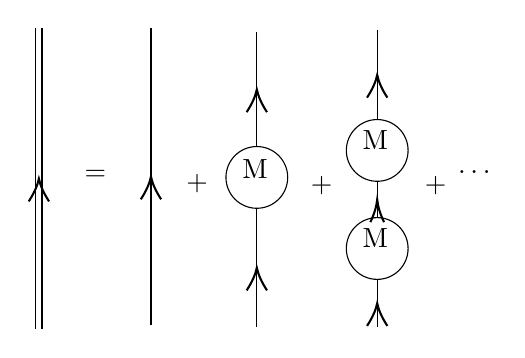
\begin{tikzpicture}[x=0.75pt,y=0.75pt,yscale=-1,xscale=1]
%uncomment if require: \path (0,300); %set diagram left start at 0, and has height of 300

%Straight Lines [id:da6679599183950475] 
\draw    (52.75,218.9) -- (52.75,73.9)(55.75,218.9) -- (55.75,73.9) ;
\draw [shift={(54.25,146.4)}, rotate = 450] [color={rgb, 255:red, 0; green, 0; blue, 0 }  ][line width=0.75]    (10.93,-4.9) .. controls (6.95,-2.3) and (3.31,-0.67) .. (0,0) .. controls (3.31,0.67) and (6.95,2.3) .. (10.93,4.9)   ;
%Straight Lines [id:da03187978212104414] 
\draw    (159.25,130.9) -- (159.25,75.9) ;
\draw [shift={(159.25,103.4)}, rotate = 450] [color={rgb, 255:red, 0; green, 0; blue, 0 }  ][line width=0.75]    (10.93,-4.9) .. controls (6.95,-2.3) and (3.31,-0.67) .. (0,0) .. controls (3.31,0.67) and (6.95,2.3) .. (10.93,4.9)   ;
%Shape: Circle [id:dp6720254680854465] 
\draw   (144.38,145.77) .. controls (144.38,137.56) and (151.03,130.9) .. (159.25,130.9) .. controls (167.47,130.9) and (174.13,137.56) .. (174.13,145.77) .. controls (174.13,153.99) and (167.47,160.65) .. (159.25,160.65) .. controls (151.03,160.65) and (144.38,153.99) .. (144.38,145.77) -- cycle ;
%Straight Lines [id:da38078856367120306] 
\draw    (159.25,160.65) -- (159.25,217.9) ;
\draw [shift={(159.25,189.27)}, rotate = 90] [color={rgb, 255:red, 0; green, 0; blue, 0 }  ][line width=0.75]    (10.93,-4.9) .. controls (6.95,-2.3) and (3.31,-0.67) .. (0,0) .. controls (3.31,0.67) and (6.95,2.3) .. (10.93,4.9)   ;
%Straight Lines [id:da45284041242528794] 
\draw    (108.25,216.9) -- (108.25,73.9) ;
\draw [shift={(108.25,145.4)}, rotate = 450] [color={rgb, 255:red, 0; green, 0; blue, 0 }  ][line width=0.75]    (10.93,-4.9) .. controls (6.95,-2.3) and (3.31,-0.67) .. (0,0) .. controls (3.31,0.67) and (6.95,2.3) .. (10.93,4.9)   ;
%Straight Lines [id:da05583872838111581] 
\draw    (217.25,117.9) -- (217.25,74.9) ;
\draw [shift={(217.25,96.4)}, rotate = 450] [color={rgb, 255:red, 0; green, 0; blue, 0 }  ][line width=0.75]    (10.93,-4.9) .. controls (6.95,-2.3) and (3.31,-0.67) .. (0,0) .. controls (3.31,0.67) and (6.95,2.3) .. (10.93,4.9)   ;
%Shape: Circle [id:dp6854080468003328] 
\draw   (202.38,132.77) .. controls (202.38,124.56) and (209.03,117.9) .. (217.25,117.9) .. controls (225.47,117.9) and (232.13,124.56) .. (232.13,132.77) .. controls (232.13,140.99) and (225.47,147.65) .. (217.25,147.65) .. controls (209.03,147.65) and (202.38,140.99) .. (202.38,132.77) -- cycle ;
%Shape: Circle [id:dp32578384863224485] 
\draw   (202.38,180.02) .. controls (202.38,171.81) and (209.03,165.15) .. (217.25,165.15) .. controls (225.47,165.15) and (232.13,171.81) .. (232.13,180.02) .. controls (232.13,188.24) and (225.47,194.9) .. (217.25,194.9) .. controls (209.03,194.9) and (202.38,188.24) .. (202.38,180.02) -- cycle ;
%Straight Lines [id:da6105349842531441] 
\draw    (217.25,165.15) -- (217.25,147.65) ;
\draw [shift={(217.25,156.4)}, rotate = 450] [color={rgb, 255:red, 0; green, 0; blue, 0 }  ][line width=0.75]    (10.93,-3.29) .. controls (6.95,-1.4) and (3.31,-0.3) .. (0,0) .. controls (3.31,0.3) and (6.95,1.4) .. (10.93,3.29)   ;
%Straight Lines [id:da308062636403606] 
\draw    (217.25,217.9) -- (217.25,194.9) ;
\draw [shift={(217.25,206.4)}, rotate = 450] [color={rgb, 255:red, 0; green, 0; blue, 0 }  ][line width=0.75]    (10.93,-4.9) .. controls (6.95,-2.3) and (3.31,-0.67) .. (0,0) .. controls (3.31,0.67) and (6.95,2.3) .. (10.93,4.9)   ;

% Text Node
\draw (75,141) node [anchor=north west][inner sep=0.75pt]   [align=left] {=};
% Text Node
\draw (124,143) node [anchor=north west][inner sep=0.75pt]   [align=left] {+};
% Text Node
\draw (184,144) node [anchor=north west][inner sep=0.75pt]   [align=left] {+};
% Text Node
\draw (239,144) node [anchor=north west][inner sep=0.75pt]   [align=left] {+};
% Text Node
\draw (255,141) node [anchor=north west][inner sep=0.75pt]    {$\dotsc $};
% Text Node
\draw (151,136) node [anchor=north west][inner sep=0.75pt]   [align=left] {M};
% Text Node
\draw (209,169) node [anchor=north west][inner sep=0.75pt]   [align=left] {M};
% Text Node
\draw (209,122) node [anchor=north west][inner sep=0.75pt]   [align=left] {M};


\end{tikzpicture}

    \caption{Partial Summation of Quantum Pinball Game}
    \label{fig:partial-sum-quantum-pinball}
\end{figure}
Convert this series to equation we have:
\begin{equation}
\begin{aligned}
G^+(\mathbf{k},\omega)&\approx G^+_0(\mathbf{k},\omega)+[G_0^+(\mathbf{k},\omega)]^2V_{M_{kk}}+[G_0^+]^3V_{M_{kk}}^2+\ldots\\
&=G_0^+(1+G_0^+V_M+(G_0^+V_M)^2+\ldots)\\
&=\frac{G_0^+(\mathbf{k},\omega)}{1-G_0^+(\mathbf{k},\omega)V_{M_{kk}}}
\end{aligned}
\end{equation}
Of course we can reproduce this calculation by manipulating the Feynman diagram series:
\begin{figure}[H]
\centering
\tikzset{every picture/.style={line width=0.75pt}} %set default line width to 0.75pt        

\begin{tikzpicture}[x=0.75pt,y=0.75pt,yscale=-1,xscale=1]
%uncomment if require: \path (0,300); %set diagram left start at 0, and has height of 300

%Straight Lines [id:da6679599183950475] 
\draw    (43.75,155.9) -- (43.75,10.9)(46.75,155.9) -- (46.75,10.9) ;
\draw [shift={(45.25,83.4)}, rotate = 450] [color={rgb, 255:red, 0; green, 0; blue, 0 }  ][line width=0.75]    (10.93,-4.9) .. controls (6.95,-2.3) and (3.31,-0.67) .. (0,0) .. controls (3.31,0.67) and (6.95,2.3) .. (10.93,4.9)   ;
%Straight Lines [id:da3819886351076084] 
\draw    (89.25,155.9) -- (89.25,12.9) ;
\draw [shift={(89.25,84.4)}, rotate = 450] [color={rgb, 255:red, 0; green, 0; blue, 0 }  ][line width=0.75]    (10.93,-4.9) .. controls (6.95,-2.3) and (3.31,-0.67) .. (0,0) .. controls (3.31,0.67) and (6.95,2.3) .. (10.93,4.9)   ;
%Straight Lines [id:da40404534625465094] 
\draw    (194.25,102.9) -- (194.25,47.9) ;
\draw [shift={(194.25,75.4)}, rotate = 450] [color={rgb, 255:red, 0; green, 0; blue, 0 }  ][line width=0.75]    (10.93,-4.9) .. controls (6.95,-2.3) and (3.31,-0.67) .. (0,0) .. controls (3.31,0.67) and (6.95,2.3) .. (10.93,4.9)   ;
%Shape: Circle [id:dp10590981200217242] 
\draw   (179.38,117.77) .. controls (179.38,109.56) and (186.03,102.9) .. (194.25,102.9) .. controls (202.47,102.9) and (209.13,109.56) .. (209.13,117.77) .. controls (209.13,125.99) and (202.47,132.65) .. (194.25,132.65) .. controls (186.03,132.65) and (179.38,125.99) .. (179.38,117.77) -- cycle ;
%Straight Lines [id:da2189214793166505] 
\draw    (259.25,100.9) -- (259.25,45.9) ;
\draw [shift={(259.25,73.4)}, rotate = 450] [color={rgb, 255:red, 0; green, 0; blue, 0 }  ][line width=0.75]    (10.93,-4.9) .. controls (6.95,-2.3) and (3.31,-0.67) .. (0,0) .. controls (3.31,0.67) and (6.95,2.3) .. (10.93,4.9)   ;
%Shape: Circle [id:dp9920078778157783] 
\draw   (244.38,115.77) .. controls (244.38,107.56) and (251.03,100.9) .. (259.25,100.9) .. controls (267.47,100.9) and (274.13,107.56) .. (274.13,115.77) .. controls (274.13,123.99) and (267.47,130.65) .. (259.25,130.65) .. controls (251.03,130.65) and (244.38,123.99) .. (244.38,115.77) -- cycle ;
%Straight Lines [id:da44750961592695404] 
\draw    (189.25,243.9) -- (189.25,218.4) ;
\draw [shift={(189.25,231.15)}, rotate = 450] [color={rgb, 255:red, 0; green, 0; blue, 0 }  ][line width=0.75]    (10.93,-4.9) .. controls (6.95,-2.3) and (3.31,-0.67) .. (0,0) .. controls (3.31,0.67) and (6.95,2.3) .. (10.93,4.9)   ;
%Shape: Circle [id:dp036519837337342875] 
\draw   (174.38,258.77) .. controls (174.38,250.56) and (181.03,243.9) .. (189.25,243.9) .. controls (197.47,243.9) and (204.13,250.56) .. (204.13,258.77) .. controls (204.13,266.99) and (197.47,273.65) .. (189.25,273.65) .. controls (181.03,273.65) and (174.38,266.99) .. (174.38,258.77) -- cycle ;
%Straight Lines [id:da9791654199909201] 
\draw    (97.25,207.02) -- (210,207.02) ;
%Straight Lines [id:da49874010942747804] 
\draw    (153.25,200.9) -- (153.25,152.4) ;
\draw [shift={(153.25,176.65)}, rotate = 450] [color={rgb, 255:red, 0; green, 0; blue, 0 }  ][line width=0.75]    (10.93,-4.9) .. controls (6.95,-2.3) and (3.31,-0.67) .. (0,0) .. controls (3.31,0.67) and (6.95,2.3) .. (10.93,4.9)   ;
%Shape: Circle [id:dp7199868696958168] 
\draw   (346.38,238.77) .. controls (346.38,230.56) and (353.03,223.9) .. (361.25,223.9) .. controls (369.47,223.9) and (376.13,230.56) .. (376.13,238.77) .. controls (376.13,246.99) and (369.47,253.65) .. (361.25,253.65) .. controls (353.03,253.65) and (346.38,246.99) .. (346.38,238.77) -- cycle ;
%Straight Lines [id:da37789491773642436] 
\draw    (271.25,205.02) -- (384,205.02) ;
%Straight Lines [id:da3979415686562028] 
\draw    (289.25,255.9) -- (289.25,217.4) ;
\draw [shift={(289.25,236.65)}, rotate = 450] [color={rgb, 255:red, 0; green, 0; blue, 0 }  ][line width=0.75]    (10.93,-4.9) .. controls (6.95,-2.3) and (3.31,-0.67) .. (0,0) .. controls (3.31,0.67) and (6.95,2.3) .. (10.93,4.9)   ;
%Straight Lines [id:da6305145122698304] 
\draw    (361.25,223.9) -- (361.25,212.4) ;
%Straight Lines [id:da6086382662478782] 
\draw    (361.25,253.65) -- (361.25,265.4) ;

% Text Node
\draw (57,77.02) node [anchor=north west][inner sep=0.75pt]  [font=\large]  {$\approx $};
% Text Node
\draw (99,81.02) node [anchor=north west][inner sep=0.75pt]    {$\times $};
% Text Node
\draw (158,83) node [anchor=north west][inner sep=0.75pt]  [font=\large] [align=left] {+};
% Text Node
\draw (186,108) node [anchor=north west][inner sep=0.75pt]   [align=left] {M};
% Text Node
\draw (137,84.02) node [anchor=north west][inner sep=0.75pt]    {$1$};
% Text Node
\draw (251,106) node [anchor=north west][inner sep=0.75pt]   [align=left] {M};
% Text Node
\draw (122,68.02) node [anchor=north west][inner sep=0.75pt]  [font=\Huge] [align=left] {[};
% Text Node
\draw (210,84) node [anchor=north west][inner sep=0.75pt]  [font=\large] [align=left] {+};
% Text Node
\draw (274,78.02) node [anchor=north west][inner sep=0.75pt]  [font=\LARGE]  {$)^{2}$};
% Text Node
\draw (228,81.02) node [anchor=north west][inner sep=0.75pt]  [font=\LARGE]  {$($};
% Text Node
\draw (308,86) node [anchor=north west][inner sep=0.75pt]  [font=\large] [align=left] {+};
% Text Node
\draw (324,90) node [anchor=north west][inner sep=0.75pt]    {$\dotsc $};
% Text Node
\draw (348,67.02) node [anchor=north west][inner sep=0.75pt]  [font=\Huge] [align=left] {]};
% Text Node
\draw (60,190.02) node [anchor=north west][inner sep=0.75pt]  [font=\large]  {$=$};
% Text Node
\draw (145,234) node [anchor=north west][inner sep=0.75pt]  [font=\Huge] [align=left] {\mbox{-}};
% Text Node
\draw (181,249) node [anchor=north west][inner sep=0.75pt]   [align=left] {M};
% Text Node
\draw (116,225.02) node [anchor=north west][inner sep=0.75pt]  [font=\LARGE]  {$1$};
% Text Node
\draw (319,232) node [anchor=north west][inner sep=0.75pt]  [font=\Huge] [align=left] {\mbox{-}};
% Text Node
\draw (353,229) node [anchor=north west][inner sep=0.75pt]   [align=left] {M};
% Text Node
\draw (318,169.02) node [anchor=north west][inner sep=0.75pt]  [font=\LARGE]  {$1$};
% Text Node
\draw (293,212.02) node [anchor=north west][inner sep=0.75pt]  [font=\Large]  {$)^{-1}$};
% Text Node
\draw (271,215.02) node [anchor=north west][inner sep=0.75pt]  [font=\Large]  {$($};
% Text Node
\draw (229,192.02) node [anchor=north west][inner sep=0.75pt]  [font=\large]  {$=$};


\end{tikzpicture}
    \caption{Diagram Calculation for the "M" Partial Summation}
    \label{fig:encircle-M-partial-summation}
\end{figure}
The diagram series above can also be rewritten in alternative form as:
\begin{center}
\tikzset{every picture/.style={line width=0.75pt}} %set default line width to 0.75pt        

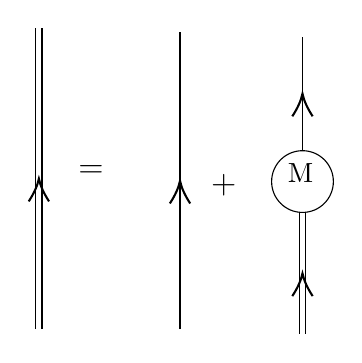
\begin{tikzpicture}[x=0.75pt,y=0.75pt,yscale=-1,xscale=1]
%uncomment if require: \path (0,300); %set diagram left start at 0, and has height of 300

%Straight Lines [id:da6679599183950475] 
\draw    (43.75,155.9) -- (43.75,10.9)(46.75,155.9) -- (46.75,10.9) ;
\draw [shift={(45.25,83.4)}, rotate = 450] [color={rgb, 255:red, 0; green, 0; blue, 0 }  ][line width=0.75]    (10.93,-4.9) .. controls (6.95,-2.3) and (3.31,-0.67) .. (0,0) .. controls (3.31,0.67) and (6.95,2.3) .. (10.93,4.9)   ;
%Straight Lines [id:da8973294663938008] 
\draw    (113.25,155.9) -- (113.25,12.9) ;
\draw [shift={(113.25,84.4)}, rotate = 450] [color={rgb, 255:red, 0; green, 0; blue, 0 }  ][line width=0.75]    (10.93,-4.9) .. controls (6.95,-2.3) and (3.31,-0.67) .. (0,0) .. controls (3.31,0.67) and (6.95,2.3) .. (10.93,4.9)   ;
%Straight Lines [id:da7528798369850997] 
\draw    (172.25,69.9) -- (172.25,14.9) ;
\draw [shift={(172.25,42.4)}, rotate = 450] [color={rgb, 255:red, 0; green, 0; blue, 0 }  ][line width=0.75]    (10.93,-4.9) .. controls (6.95,-2.3) and (3.31,-0.67) .. (0,0) .. controls (3.31,0.67) and (6.95,2.3) .. (10.93,4.9)   ;
%Shape: Circle [id:dp7507000793435626] 
\draw   (157.38,84.77) .. controls (157.38,76.56) and (164.03,69.9) .. (172.25,69.9) .. controls (180.47,69.9) and (187.13,76.56) .. (187.13,84.77) .. controls (187.13,92.99) and (180.47,99.65) .. (172.25,99.65) .. controls (164.03,99.65) and (157.38,92.99) .. (157.38,84.77) -- cycle ;
%Straight Lines [id:da663573424332869] 
\draw    (173.75,99.65) -- (173.75,158.4)(170.75,99.65) -- (170.75,158.4) ;
\draw [shift={(172.25,129.02)}, rotate = 90] [color={rgb, 255:red, 0; green, 0; blue, 0 }  ][line width=0.75]    (10.93,-4.9) .. controls (6.95,-2.3) and (3.31,-0.67) .. (0,0) .. controls (3.31,0.67) and (6.95,2.3) .. (10.93,4.9)   ;

% Text Node
\draw (63,76.02) node [anchor=north west][inner sep=0.75pt]  [font=\large]  {$=$};
% Text Node
\draw (164,75) node [anchor=north west][inner sep=0.75pt]   [align=left] {M};
% Text Node
\draw (127,80) node [anchor=north west][inner sep=0.75pt]  [font=\large] [align=left] {+};


\end{tikzpicture}

\end{center}
Finally, we substitute for $G_{0}^{+}$ and for $V_{M}$ and obtain:
\begin{equation}G^{+}(\mathbf{k}, \omega)=\frac{1}{\omega-\epsilon_{k}+i \delta-V_{M_{k k}}}=\frac{1}{\omega-\left(\epsilon_{k}+M k^{2}\right)+i \delta}\end{equation}
Comparing this with the quasi particle propagator we find
\begin{equation}\begin{array}{l}
\epsilon_{k}^{\prime}=\epsilon_{k}+M k^{2}=\left(\frac{1}{2 m}+M\right) k^{2} \\
\tau_{k}=\frac{1}{\delta}=\infty
\end{array}\end{equation}

If we consider $V_L$, we calculate the whole diagram series as 
\begin{center}
\tikzset{every picture/.style={line width=0.75pt}} %set default line width to 0.75pt        

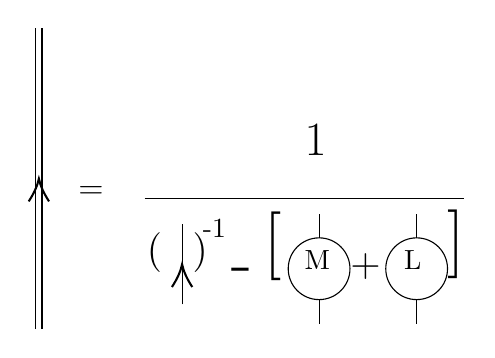
\begin{tikzpicture}[x=0.75pt,y=0.75pt,yscale=-1,xscale=1]
%uncomment if require: \path (0,300); %set diagram left start at 0, and has height of 300

%Straight Lines [id:da6679599183950475] 
\draw    (21.75,153.9) -- (21.75,8.9)(24.75,153.9) -- (24.75,8.9) ;
\draw [shift={(23.25,81.4)}, rotate = 450] [color={rgb, 255:red, 0; green, 0; blue, 0 }  ][line width=0.75]    (10.93,-4.9) .. controls (6.95,-2.3) and (3.31,-0.67) .. (0,0) .. controls (3.31,0.67) and (6.95,2.3) .. (10.93,4.9)   ;
%Shape: Circle [id:dp8530247155182938] 
\draw   (143.38,124.77) .. controls (143.38,116.56) and (150.03,109.9) .. (158.25,109.9) .. controls (166.47,109.9) and (173.13,116.56) .. (173.13,124.77) .. controls (173.13,132.99) and (166.47,139.65) .. (158.25,139.65) .. controls (150.03,139.65) and (143.38,132.99) .. (143.38,124.77) -- cycle ;
%Straight Lines [id:da5960930796514846] 
\draw    (74.25,91.02) -- (228.25,91.02) ;
%Straight Lines [id:da5321584258205649] 
\draw    (92.25,141.9) -- (92.25,103.4) ;
\draw [shift={(92.25,122.65)}, rotate = 450] [color={rgb, 255:red, 0; green, 0; blue, 0 }  ][line width=0.75]    (10.93,-4.9) .. controls (6.95,-2.3) and (3.31,-0.67) .. (0,0) .. controls (3.31,0.67) and (6.95,2.3) .. (10.93,4.9)   ;
%Straight Lines [id:da11643204321065659] 
\draw    (158.25,109.9) -- (158.25,98.4) ;
%Straight Lines [id:da8969952308596885] 
\draw    (158.25,139.65) -- (158.25,151.4) ;
%Shape: Circle [id:dp18446767982176082] 
\draw   (190.38,124.77) .. controls (190.38,116.56) and (197.03,109.9) .. (205.25,109.9) .. controls (213.47,109.9) and (220.13,116.56) .. (220.13,124.77) .. controls (220.13,132.99) and (213.47,139.65) .. (205.25,139.65) .. controls (197.03,139.65) and (190.38,132.99) .. (190.38,124.77) -- cycle ;
%Straight Lines [id:da2983905665141421] 
\draw    (205.25,109.9) -- (205.25,98.4) ;
%Straight Lines [id:da04673018570564247] 
\draw    (205.25,139.65) -- (205.25,151.4) ;

% Text Node
\draw (41,84.02) node [anchor=north west][inner sep=0.75pt]  [font=\large]  {$=$};
% Text Node
\draw (115,117) node [anchor=north west][inner sep=0.75pt]  [font=\Huge] [align=left] {\mbox{-}};
% Text Node
\draw (150,115) node [anchor=north west][inner sep=0.75pt]   [align=left] {M};
% Text Node
\draw (150,54.02) node [anchor=north west][inner sep=0.75pt]  [font=\LARGE]  {$1$};
% Text Node
\draw (96,106.02) node [anchor=north west][inner sep=0.75pt]  [font=\Large]  {$)$};
% Text Node
\draw (74,106.02) node [anchor=north west][inner sep=0.75pt]  [font=\Large]  {$($};
% Text Node
\draw (198,115) node [anchor=north west][inner sep=0.75pt]   [align=left] {L};
% Text Node
\draw (172,116) node [anchor=north west][inner sep=0.75pt]  [font=\Large] [align=left] {+};
% Text Node
\draw (130.6,96.02) node [anchor=north west][inner sep=0.75pt]  [font=\Huge] [align=left] {[};
% Text Node
\draw (218.65,95.02) node [anchor=north west][inner sep=0.75pt]  [font=\Huge] [align=left] {]};
% Text Node
\draw (101,100.02) node [anchor=north west][inner sep=0.75pt]   [align=left] {\mbox{-}1};


\end{tikzpicture}

\end{center}
or, translating:
\begin{equation}G^{+}(\mathbf{k}, \omega)=\frac{1}{\left(G_{0}^{+}\right)^{-1}-\left(V_{M_{k k}}+V_{L_{k k}}\right)}=\frac{1}{\omega-\left(\frac{k^{2}}{2 m}+M k^{2}+L k^{4}\right)+i \delta}\end{equation}

\subsection{Where the diagram expansion or the propagator really comes from}
We will now show in a rough way how the diagram expansion of $G^{+}$ in this single-particle case can be gotten from the Schrodinger equation. The first thing to realize is that \textbf{$G_{0}^{+}$ and $G^{+}$ are actually Green's functions}. Recall that if we have a differential equation of the form
\begin{equation}L \psi(\mathbf{x}, t)=f(\mathbf{x}, t)
\label{diagram-expand-exp-1}
\end{equation}
where $L$ is a linear differential operator which does not depend explicitly on $x$ or $t,$ then the Green's function, $G,$ associated with this equation is the solution of
\begin{equation}L G\left(\mathbf{x}-\mathbf{x}^{\prime}, t-t^{\prime}\right)=\delta\left(\mathbf{x}-\mathbf{x}^{\prime}\right) \delta\left(t-t^{\prime}\right)
\label{diagram-expand-exp-2}
\end{equation}
Now the unperturbed Schrodinger equation may be written
$$\left(+\frac{\nabla^{2}}{2 m}+i \frac{\partial}{\partial t}\right) \psi(\mathbf{x}, t)=0$$
Thus, the associated Green's function obeys
\begin{equation}\left(+\frac{\nabla^{2}}{2 m}+i \frac{\partial}{\partial t}\right) G\left(\mathbf{x}-\mathbf{x}^{\prime}, t-t^{\prime}\right)=\delta\left(\mathbf{x}-\mathbf{x}^{\prime}\right)\delta\left(t-t^{\prime}\right)
\label{diagram-expand-exp-3}
\end{equation}
Since
\begin{equation}G\left(x-x^{\prime}, t-t^{\prime}\right)=\int \frac{d^{3} k}{(2 \pi)^{3}} e^{i k \cdot\left(x-x^{\prime}\right)} G\left(k, t-t^{\prime}\right)
\label{diagram-expand-exp-4}
\end{equation}
and using the Fourier transform of $\delta(x-x^{\prime})$ we find that
\begin{equation}\left(-\frac{k^{2}}{2 m}+i \frac{\partial}{\partial t}\right) G\left(\mathbf{k}, t-t^{\prime}\right)=\delta\left(t-t^{\prime}\right)
\label{diagram-expand-exp-5}
\end{equation}
If we use the fact that
\begin{imp}
\begin{equation}\frac{d \theta_{x}}{d x}=\delta(x), \quad f(x) \delta(x)=f(0) \delta(x)
\label{diagram-expand-exp-6}
\end{equation}
\end{imp}
and substitute $G^+_0(\mathbf{k},\omega)=-i\theta_{t-t^{\prime}}e^{-i\epsilon_k(t=t^{\prime})}$ into (\ref{diagram-expand-exp-5}), we find the $G_0^+$ is satisfied.

In a similar way, the Shrodinger equation with a perturbing potential $V(\nabla)$
\begin{equation}\left[+\frac{\nabla^{2}}{2 m}+i \frac{\partial}{\partial t}-V(\nabla)\right] \psi(\mathbf{x}, t)=0\end{equation}
has associated Green's function as
\begin{equation}\left[-\frac{k^{2}}{2 m}+i \frac{\partial}{\partial t}-V(\mathbf{k})\right] G^{+}\left(\mathbf{k}, t-t^{\prime}\right)=\delta\left(t-t^{\prime}\right)
\label{diagram-expand-7}
\end{equation}
where $V(\mathbf{k})$ is the Fourier transform of $V(\nabla) .$ The solution to this may be written as an integral equation
\begin{equation}\boldsymbol{G}^{+}\left(\mathbf{k}, t-t^{\prime}\right)=G_{\mathbf{0}}^{+}\left(\mathbf{k}, t-t^{\prime}\right)+\int_{-\infty}^{+\infty} d t^{*} G_{0}^{+}\left(\mathbf{k}, t-t^{*}\right) V(\mathbf{k}) G^{+}\left(\mathbf{k}, t^{*}-t^{\prime}\right)
\label{diagram-expand-exp-8}
\end{equation}
This can be seen by substituting (\ref{diagram-expand-exp-8}) into (\ref{diagram-expand-7}) and use (\ref{diagram-expand-exp-5}) with $G=G^+_0$.Expanding the (\ref{diagram-expand-exp-8}) we recover the series in spacetime.

\subsection{Energy and lifetime of an electron In an Impure metal}
We will now apply the propagator method to a more realistic problem, i.e., an electron in an impure metal. For simplicity, Jet us pretend that the regularly arranged lattice ions in the metal have been removed, so that all we have left is an electron interacting with a set of N randomly distributed impurity ions, which are identical in a volume $\Omega$. If we use $\mathbf{R}_i$ to represent ion coordinates, then the potential well for an impurity at the $\mathbf{R_i}$ has the form of $W(\mathbf{r}-\mathbf{R}_i)$. Recall that $\phi(\mathbf{r})=e^{-i\mathbf{k\cdot r}}$, we have the matrix element of transitioning amplitude from $\mathbf{k}$ to $\mathbf{l}$ at $R_i$ as
\begin{equation}-i V_{\mathbf{lk}}\left(\mathbf{R}_{i}\right)=\frac{-i}{\Omega} \int d^{3} \mathbf{r} e^{-i(\mathbf{l}-\mathbf{k}) \cdot \mathbf{r}} \mathbf{W}\left(\mathbf{r}-\mathbf{R}_{i}\right)
\label{W-potential-amplitude}
\end{equation}
\redp{Now using $\mathbf{r}^{\prime}=\mathbf{r}-\mathbf{R}_i$}, we have (\ref{W-potential-amplitude}) becomes
\begin{equation}
    -iV_{\mathbf{lk}}=\frac{(-i)}{\Omega} e^{-i(\mathbf{l-k}) \cdot \mathbf{R}_{i}} \mathbf{W}_{l k}
    \label{W-potential-amplitude-2}
\end{equation}
where
$$W_{l k}=\int d^{3} \mathbf{r}^{\prime} e^{-i(\mathbf{l}-\mathbf{k}) \cdot \mathbf{r}^{\prime}} W\left(\mathbf{r}^{\prime}\right)$$
After eliminating the $i$ 's and suppressing $\omega$ 's for brevity, (noting that it is necessary to sum over all values of the intermediate momentum, $\mathbf{l}$) we have:
\begin{equation}\begin{aligned}
G^{+}\left(\mathbf{k}_{2}, \mathbf{k}_{1}\right)=& G_{0}^{+}\left(\mathbf{k}_{1}\right) \delta_{k_{1} k_{2}}+G_{0}^{+}\left(\mathbf{k}_{2}\right) \sum_{t=1}^{N} V_{k_{2} k_{1}}\left(\mathbf{R}_{i}\right) G_{0}^{+}\left(\mathbf{k}_{1}\right)+\\
&+G_{0}^{+}\left(\mathbf{k}_{2}\right)\left[\sum_{l} \sum_{i=1}^{N} V_{k_{2} l}\left(\mathbf{R}_{i}\right) G_{0}^{+}(\mathbf{l}) V_{l k_{1}}\left(\mathbf{R}_{i}\right)\right] G_{0}^{+}\left(\mathbf{k}_{1}\right)+\\
&+G_{0}^{+}\left(\mathbf{k}_{2}\right)\left[\sum_{l} \sum_{j \neq 1} V_{k_{2} l}\left(\mathbf{R}_{j}\right) G_{0}^{+}(\mathbf{l}) \sum_{i=1}^{N} V_{l k_{1}}\left(\mathbf{R}_{l}\right)\right] G_{0}^{+}\left(\mathbf{k}_{1}\right)+\cdots
\end{aligned}
\label{impurity-ion-amp-expansion}
\end{equation}
The above $G^{+}$ is for a particular set of $\mathbf{R}_{i}$ 's, and for each different set of $\mathbf{R}_{t}^{\prime}$ 's, we will get a different value of $G^{+} .$ Consider now an \bluep{ensemble consisting of all possible arrangements of impurities}. Suppose this ensemble is random, i.e., \textbf{the coordinate for the ith impurtity, $\mathbf{R}_{\mathbf{i}}$, is equally likely to be found anywhere in the volume $\Omega$.} Let us imagine that we compute $\left\langle G^{+}\right\rangle,$ the average value of $G^{+}$ for the ensemble. Clearly, for any specific arrangement, $G^{+} \neq\left\langle G^{+}\right\rangle .$ But, \redp{as is common in large systems, in the limit $N \rightarrow \infty$ (with $N / \Omega=\text { constant }),$ the ratio of the mean square fluctuation $\left(\left\langle G^{+2}\right\rangle-\left\langle G^{+}\right\rangle^{2}\right)$ to $\left\langle G^{+}\right\rangle^{2}$ will go to zero, \textbf{so that we can take $G^{+}=\left\langle G^{+}\right\rangle$ for all but a negligible number of arrangements (see Kohn and Luttinger (1957))}}. Hence our object here will be to calculate $\langle G^+\rangle$.

From \ref{impurity-ion-amp-expansion}, we have
\begin{equation}\left\langle G_{0}^{+}\left(\mathbf{k}_{2}\right) G_{0}^{+}\left(\mathbf{k}_{1}\right) \sum_{i=1}^{N} V_{k_{2} k_{1}}\left(\mathbf{R}_{i}\right)\right\rangle=G_{0}^{+}\left(\mathbf{k}_{2}\right) G_{0}^{+}\left(\mathbf{k}_{1}\right) \frac{W_{k_{2} k_{1}}}{\Omega}\left\langle\sum_{i=1}^{N} e^{-i\left(\mathbf{k}_{2}-\mathbf{k}_{1}\right) \cdot \mathbf{r}_{i}}\right\rangle
\label{impurity-1-avg}
\end{equation}
where
\begin{equation}\left\langle\sum_{t=1}^{N} e^{-i\left(\mathbf{k}_{2}-\mathbf{k}_{1}\right) \cdot \mathbf{R}_{i}}\right\rangle=\sum_{i=1}^{N} \langle e^{-i(\mathbf{k}_{2}-\mathbf{k}_{1}) \cdot \mathbf{R}_{i}}\rangle=N\langle e^{-i(\mathbf{k}_{2}-\mathbf{k}_{1}) \cdot \mathbf{R}_{i}}\rangle
\end{equation}
Since the distribution of the ions is totally random, we have
\begin{equation}
\langle e^{-i(\mathbf{k}_{2}-\mathbf{k}_{1}) \cdot \mathbf{R}_{i}}\rangle=\frac{1}{\Omega} \int d^{3} \mathbf{R}_{i} e^{-i\left(\mathbf{k}_{2}-\mathbf{k}_{1}\right) \cdot \mathbf{R}_{i}}=\frac{1}{\Omega} \times \Omega \delta_{\mathbf{k}_{2} \mathbf{k}_{1}}
\label{random-avg}
\end{equation}
\begin{mybox}
In a one-dimensional box of length $L$,
$$I \equiv \int_{-L / 2}^{+L / 2} d x \exp (-i k x)=2 k^{-1} \sin (k L / 2)$$
Because of periodic boundary conditions, the wave function at $x=0$ equals that at $x=L,$ i.e., $\exp (i k x)=\exp (i k(x+L)) .$ Hence $\exp (i k L)=1,$ or $k=2 \pi n / L$
$(n=\text { integer }) .$ Thus $I=L \delta_{k, 0} .$ Equation (\ref{random-avg}) is just the three-dimensional version of this with $\Omega=L^3$. If $\mathbf{k}$ is continuous, the integral (\ref{random-avg}) yields $(2 \pi)^{3} \delta\left(\mathbf{k}_{2}-\mathbf{k}_{1}\right),$ which is a Dirac $\delta$ -function.
\end{mybox}
Similarly, for successive scattering on the same ion, we have
\begin{equation}
    \begin{aligned}
\sum_{l} G_{0}^{+}(\mathbf{l})\left\langle\sum_{i} V_{\mathrm{k}_{2} l}\left(\mathrm{R}_{i}\right) V_{lk_{1}}\left(\mathrm{R}_{i}\right)\right\rangle &=\sum_{\mathbf{l}} G_{0}^{+}(\mathbf{l}) \frac{W_{\mathrm{k}_{2} l} W_{\mathrm{lk_1}}}{\Omega^{2}}\left\langle\sum_{\mathrm{i}} e^{-i\left(k_{2}-l+l-\mathrm{k}_{1}\right) \cdot R_{i}}\right\rangle \\
&=\frac{N}{\Omega^{2}} \sum_{l} G_{0}^{+}(\mathbf{l}) W_{\mathrm{k}_{2} l} W_{l k_{1}} \delta_{\mathrm{k}_{2} \mathrm{k}_{1}}
\end{aligned}
\label{impurity-1st-avg}
\end{equation}
It is usually more convenient to change from a sum over $\mathbf{l}$ to an integral by
\begin{imp}
\begin{equation}\sum_{l} \rightarrow \frac{\Omega}{(2 \pi)^{3}} \int d^{3} \mathbf{l}\end{equation}
The factor $\Omega /(2 \pi)^{3}$ is the density of points in $\mathrm{k}$ -space. To see this, we note that in one dimension, $k=2 \pi n / L$ $(n=\text { integer }) .$ Thus there are $L / 2 \pi$ points per unit length in $\mathbf{k}-$space in one dimension. In three dimensions we have $L^3/(2\pi)^3=\Omega/(2\pi)^3$ points per unit volume in $\mathbf{k}-$space.
\end{imp}
\ref{impurity-1st-avg} now becomes
$$=\frac{N}{\Omega} \int \frac{d^{3} \mathbf{l}}{(2 \pi)^{3}} G_{0}^{+}(1) W_{k_{2}l} W_{l k_{1}} \delta_{k_{2} k_{1}}$$
The two successive scattering term from different ions contains the average 
$$\begin{array}{l}
\sum_{l} G_{0}^{+}(l)\left\langle\sum_{l, j\neq i} V_{k_{2} l}\left(R_{i}\right) V_{lk_1}{\left(R_{i}\right)}\right\rangle \\
\quad=\sum_{l} G_{0}^{+}(l) \frac{W_{k_{2} l} W_{l k_{1}}}{\Omega^{2}}\left\langle\sum_{l, j \neq i} e^{-i\left(k_{2}-\mathbf{l}\right) \cdot R_{j}} e^{-i\left(\mathbf{l}-k_{1}\right) \cdot R_{i}}\right)\\
\quad=\sum_{l} G_{0}^{+}(1) \frac{W_{k_{2} l} W_{l k_{1}}}{\Omega^{2}} N(N-1)\int \frac{d^{3} \mathbf{R}_{j}}{\Omega} \int \frac{d^{3} \mathbf{R}_{i}}{\Omega}e^{-i\left(k_{2}-\mathbf{l}\right) \cdot R_{j}} e^{-i(\mathbf{l}-k_{1}) \cdot R_{i}})\\
\quad\approx\left(\frac{N}{\Omega}\right)^{2} \sum_{l} G_{0}^{+}(l) W_{k_{2} l} W_{l k_{1}} \delta_{k_{2} l} \delta_{l k_{2}}\\
\quad=\left(\frac{N}{\Omega}\right)^{2} G_{0}^{+}\left(\mathbf{k}_{1}\right) W_{k_{1} k_{1}}^{2} \delta_{k_{2} k_{1}}
\end{array}$$
With the aid of these results, we can write out the series for the averaged propagator. It helps here to introduce a couple of new diagram conventions. First of all, we use just an empty circle to represent $V_{lk}(\mathbf{R}_i)$, for the transition probability amplitude $W_{lk}$ Secondly, \bluep{\textbf{because each group of two or more successive scatterings at the same ion has an associated density factor $N/\Omega$,}} we connect successive circles representing the same ion by dotted
lines. (Note that a single scattering also has this factor associated with it.) Thus, taking the $\delta$-functions into account, and letting $\mathbf{k}_1=\mathbf{k}=\mathbf{k}_2$, we have for the averaged propagator:

\begin{equation}
    \tikzset{every picture/.style={line width=0.75pt}} %set default line width to 0.75pt        
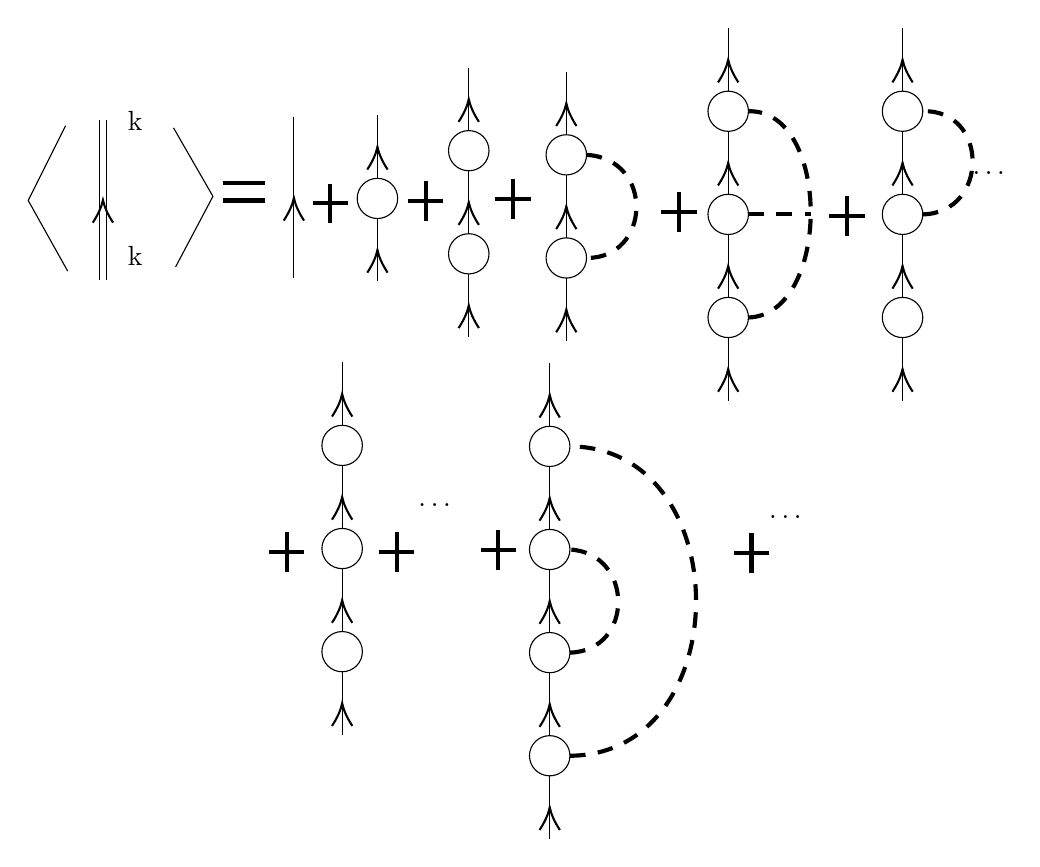
\begin{tikzpicture}[x=0.75pt,y=0.75pt,yscale=-1,xscale=1]
%uncomment if require: \path (0,410); %set diagram left start at 0, and has height of 410

%Straight Lines [id:da6679599183950475] 
\draw    (42.75,129.9) -- (42.75,52.4)(45.75,129.9) -- (45.75,52.4) ;
\draw [shift={(44.25,91.15)}, rotate = 450] [color={rgb, 255:red, 0; green, 0; blue, 0 }  ][line width=0.75]    (10.93,-4.9) .. controls (6.95,-2.3) and (3.31,-0.67) .. (0,0) .. controls (3.31,0.67) and (6.95,2.3) .. (10.93,4.9)   ;
%Straight Lines [id:da96866989164835] 
\draw    (78.25,56.4) -- (97.25,89.4) -- (79.25,123.4) ;
%Straight Lines [id:da6934326937577064] 
\draw    (26.25,55.4) -- (8.25,91.4) -- (27.25,125.4) ;
%Straight Lines [id:da3013274600825496] 
\draw [line width=1.5]    (102,83.02) -- (122.25,83.02) ;
%Straight Lines [id:da002431265709683772] 
\draw [line width=1.5]    (102,91.4) -- (122.25,91.4) ;

%Straight Lines [id:da5008643601850559] 
\draw    (136.25,128.9) -- (136.25,51.4) ;
\draw [shift={(136.25,90.15)}, rotate = 450] [color={rgb, 255:red, 0; green, 0; blue, 0 }  ][line width=0.75]    (10.93,-4.9) .. controls (6.95,-2.3) and (3.31,-0.67) .. (0,0) .. controls (3.31,0.67) and (6.95,2.3) .. (10.93,4.9)   ;
%Straight Lines [id:da6945756947603086] 
\draw    (176.5,80.72) -- (176.5,50.4) ;
\draw [shift={(176.5,65.56)}, rotate = 450] [color={rgb, 255:red, 0; green, 0; blue, 0 }  ][line width=0.75]    (10.93,-4.9) .. controls (6.95,-2.3) and (3.31,-0.67) .. (0,0) .. controls (3.31,0.67) and (6.95,2.3) .. (10.93,4.9)   ;
%Shape: Ellipse [id:dp3530646460829052] 
\draw   (166.75,90.4) .. controls (166.75,85.05) and (171.12,80.72) .. (176.5,80.72) .. controls (181.88,80.72) and (186.25,85.05) .. (186.25,90.4) .. controls (186.25,95.75) and (181.88,100.08) .. (176.5,100.08) .. controls (171.12,100.08) and (166.75,95.75) .. (166.75,90.4) -- cycle ;
%Straight Lines [id:da43208207245118435] 
\draw    (176.5,130.4) -- (176.5,100.08) ;
\draw [shift={(176.5,115.24)}, rotate = 450] [color={rgb, 255:red, 0; green, 0; blue, 0 }  ][line width=0.75]    (10.93,-4.9) .. controls (6.95,-2.3) and (3.31,-0.67) .. (0,0) .. controls (3.31,0.67) and (6.95,2.3) .. (10.93,4.9)   ;

%Straight Lines [id:da7828111751257385] 
\draw    (220.5,57.72) -- (220.5,27.4) ;
\draw [shift={(220.5,42.56)}, rotate = 450] [color={rgb, 255:red, 0; green, 0; blue, 0 }  ][line width=0.75]    (10.93,-4.9) .. controls (6.95,-2.3) and (3.31,-0.67) .. (0,0) .. controls (3.31,0.67) and (6.95,2.3) .. (10.93,4.9)   ;
%Shape: Ellipse [id:dp6295020134353576] 
\draw   (210.75,67.4) .. controls (210.75,62.05) and (215.12,57.72) .. (220.5,57.72) .. controls (225.88,57.72) and (230.25,62.05) .. (230.25,67.4) .. controls (230.25,72.75) and (225.88,77.08) .. (220.5,77.08) .. controls (215.12,77.08) and (210.75,72.75) .. (210.75,67.4) -- cycle ;
%Straight Lines [id:da5190411567838193] 
\draw    (220.5,107.4) -- (220.5,77.08) ;
\draw [shift={(220.5,92.24)}, rotate = 450] [color={rgb, 255:red, 0; green, 0; blue, 0 }  ][line width=0.75]    (10.93,-4.9) .. controls (6.95,-2.3) and (3.31,-0.67) .. (0,0) .. controls (3.31,0.67) and (6.95,2.3) .. (10.93,4.9)   ;

%Shape: Ellipse [id:dp1856254885258023] 
\draw   (210.75,117.08) .. controls (210.75,111.74) and (215.12,107.4) .. (220.5,107.4) .. controls (225.88,107.4) and (230.25,111.74) .. (230.25,117.08) .. controls (230.25,122.43) and (225.88,126.77) .. (220.5,126.77) .. controls (215.12,126.77) and (210.75,122.43) .. (210.75,117.08) -- cycle ;
%Straight Lines [id:da12064415501164083] 
\draw    (220.5,157.08) -- (220.5,126.77) ;
\draw [shift={(220.5,141.93)}, rotate = 450] [color={rgb, 255:red, 0; green, 0; blue, 0 }  ][line width=0.75]    (10.93,-4.9) .. controls (6.95,-2.3) and (3.31,-0.67) .. (0,0) .. controls (3.31,0.67) and (6.95,2.3) .. (10.93,4.9)   ;
%Straight Lines [id:da7079596940921928] 
\draw    (267.5,59.72) -- (267.5,29.4) ;
\draw [shift={(267.5,44.56)}, rotate = 450] [color={rgb, 255:red, 0; green, 0; blue, 0 }  ][line width=0.75]    (10.93,-4.9) .. controls (6.95,-2.3) and (3.31,-0.67) .. (0,0) .. controls (3.31,0.67) and (6.95,2.3) .. (10.93,4.9)   ;
%Shape: Ellipse [id:dp22478419986022313] 
\draw   (257.75,69.4) .. controls (257.75,64.05) and (262.12,59.72) .. (267.5,59.72) .. controls (272.88,59.72) and (277.25,64.05) .. (277.25,69.4) .. controls (277.25,74.75) and (272.88,79.08) .. (267.5,79.08) .. controls (262.12,79.08) and (257.75,74.75) .. (257.75,69.4) -- cycle ;
%Straight Lines [id:da11608178895592369] 
\draw    (267.5,109.4) -- (267.5,79.08) ;
\draw [shift={(267.5,94.24)}, rotate = 450] [color={rgb, 255:red, 0; green, 0; blue, 0 }  ][line width=0.75]    (10.93,-4.9) .. controls (6.95,-2.3) and (3.31,-0.67) .. (0,0) .. controls (3.31,0.67) and (6.95,2.3) .. (10.93,4.9)   ;

%Shape: Ellipse [id:dp33421438233375045] 
\draw   (257.75,119.08) .. controls (257.75,113.74) and (262.12,109.4) .. (267.5,109.4) .. controls (272.88,109.4) and (277.25,113.74) .. (277.25,119.08) .. controls (277.25,124.43) and (272.88,128.77) .. (267.5,128.77) .. controls (262.12,128.77) and (257.75,124.43) .. (257.75,119.08) -- cycle ;
%Straight Lines [id:da8470461387935158] 
\draw    (267.5,159.08) -- (267.5,128.77) ;
\draw [shift={(267.5,143.93)}, rotate = 450] [color={rgb, 255:red, 0; green, 0; blue, 0 }  ][line width=0.75]    (10.93,-4.9) .. controls (6.95,-2.3) and (3.31,-0.67) .. (0,0) .. controls (3.31,0.67) and (6.95,2.3) .. (10.93,4.9)   ;
%Straight Lines [id:da5580045724596926] 
\draw [line width=1.5]    (145.25,92.8) -- (162.25,92.8) ;
%Straight Lines [id:da21350536390327923] 
\draw [line width=1.5]    (153.75,102.4) -- (153.75,83.21) ;

%Straight Lines [id:da8624253903000908] 
\draw [line width=1.5]    (191.25,91.8) -- (208.25,91.8) ;
%Straight Lines [id:da39200924475692256] 
\draw [line width=1.5]    (199.75,101.4) -- (199.75,82.21) ;

%Straight Lines [id:da11442905940915027] 
\draw [line width=1.5]    (233.25,90.8) -- (250.25,90.8) ;
%Straight Lines [id:da6458220565812314] 
\draw [line width=1.5]    (241.75,100.4) -- (241.75,81.21) ;

%Curve Lines [id:da5905027576335966] 
\draw [line width=1.5]  [dash pattern={on 5.63pt off 4.5pt}]  (277.25,69.4) .. controls (310.25,71.4) and (308.25,119.4) .. (277.25,119.08) ;
%Straight Lines [id:da9968425195966377] 
\draw    (345.5,38.72) -- (345.5,8.4) ;
\draw [shift={(345.5,23.56)}, rotate = 450] [color={rgb, 255:red, 0; green, 0; blue, 0 }  ][line width=0.75]    (10.93,-4.9) .. controls (6.95,-2.3) and (3.31,-0.67) .. (0,0) .. controls (3.31,0.67) and (6.95,2.3) .. (10.93,4.9)   ;
%Shape: Ellipse [id:dp9509322965168189] 
\draw   (335.75,48.4) .. controls (335.75,43.05) and (340.12,38.72) .. (345.5,38.72) .. controls (350.88,38.72) and (355.25,43.05) .. (355.25,48.4) .. controls (355.25,53.75) and (350.88,58.08) .. (345.5,58.08) .. controls (340.12,58.08) and (335.75,53.75) .. (335.75,48.4) -- cycle ;
%Straight Lines [id:da08673873782145747] 
\draw    (345.5,88.4) -- (345.5,58.08) ;
\draw [shift={(345.5,73.24)}, rotate = 450] [color={rgb, 255:red, 0; green, 0; blue, 0 }  ][line width=0.75]    (10.93,-4.9) .. controls (6.95,-2.3) and (3.31,-0.67) .. (0,0) .. controls (3.31,0.67) and (6.95,2.3) .. (10.93,4.9)   ;

%Shape: Ellipse [id:dp8921785518031183] 
\draw   (335.75,98.08) .. controls (335.75,92.74) and (340.12,88.4) .. (345.5,88.4) .. controls (350.88,88.4) and (355.25,92.74) .. (355.25,98.08) .. controls (355.25,103.43) and (350.88,107.77) .. (345.5,107.77) .. controls (340.12,107.77) and (335.75,103.43) .. (335.75,98.08) -- cycle ;
%Straight Lines [id:da5781140789642911] 
\draw    (345.5,138.08) -- (345.5,107.77) ;
\draw [shift={(345.5,122.93)}, rotate = 450] [color={rgb, 255:red, 0; green, 0; blue, 0 }  ][line width=0.75]    (10.93,-4.9) .. controls (6.95,-2.3) and (3.31,-0.67) .. (0,0) .. controls (3.31,0.67) and (6.95,2.3) .. (10.93,4.9)   ;
%Shape: Ellipse [id:dp9670986903241016] 
\draw   (335.75,147.77) .. controls (335.75,142.42) and (340.12,138.08) .. (345.5,138.08) .. controls (350.88,138.08) and (355.25,142.42) .. (355.25,147.77) .. controls (355.25,153.12) and (350.88,157.45) .. (345.5,157.45) .. controls (340.12,157.45) and (335.75,153.12) .. (335.75,147.77) -- cycle ;
%Straight Lines [id:da9751245477461478] 
\draw    (345.5,187.77) -- (345.5,157.45) ;
\draw [shift={(345.5,172.61)}, rotate = 450] [color={rgb, 255:red, 0; green, 0; blue, 0 }  ][line width=0.75]    (10.93,-4.9) .. controls (6.95,-2.3) and (3.31,-0.67) .. (0,0) .. controls (3.31,0.67) and (6.95,2.3) .. (10.93,4.9)   ;
%Curve Lines [id:da845705807763435] 
\draw [line width=1.5]  [dash pattern={on 5.63pt off 4.5pt}]  (355.25,147.77) .. controls (395.25,146.4) and (395.25,47.4) .. (355.25,48.4) ;
%Straight Lines [id:da3256851388470269] 
\draw [line width=1.5]  [dash pattern={on 5.63pt off 4.5pt}]  (355.25,98.08) -- (385.25,98.08) ;
%Straight Lines [id:da09806150660985813] 
\draw [line width=1.5]    (313.25,96.8) -- (330.25,96.8) ;
%Straight Lines [id:da8319212817021413] 
\draw [line width=1.5]    (321.75,106.4) -- (321.75,87.21) ;

%Straight Lines [id:da17267749447821656] 
\draw    (429.5,38.72) -- (429.5,8.4) ;
\draw [shift={(429.5,23.56)}, rotate = 450] [color={rgb, 255:red, 0; green, 0; blue, 0 }  ][line width=0.75]    (10.93,-4.9) .. controls (6.95,-2.3) and (3.31,-0.67) .. (0,0) .. controls (3.31,0.67) and (6.95,2.3) .. (10.93,4.9)   ;
%Shape: Ellipse [id:dp6338000815403856] 
\draw   (419.75,48.4) .. controls (419.75,43.05) and (424.12,38.72) .. (429.5,38.72) .. controls (434.88,38.72) and (439.25,43.05) .. (439.25,48.4) .. controls (439.25,53.75) and (434.88,58.08) .. (429.5,58.08) .. controls (424.12,58.08) and (419.75,53.75) .. (419.75,48.4) -- cycle ;
%Straight Lines [id:da6359368270166951] 
\draw    (429.5,88.4) -- (429.5,58.08) ;
\draw [shift={(429.5,73.24)}, rotate = 450] [color={rgb, 255:red, 0; green, 0; blue, 0 }  ][line width=0.75]    (10.93,-4.9) .. controls (6.95,-2.3) and (3.31,-0.67) .. (0,0) .. controls (3.31,0.67) and (6.95,2.3) .. (10.93,4.9)   ;

%Shape: Ellipse [id:dp8160936873445316] 
\draw   (419.75,98.08) .. controls (419.75,92.74) and (424.12,88.4) .. (429.5,88.4) .. controls (434.88,88.4) and (439.25,92.74) .. (439.25,98.08) .. controls (439.25,103.43) and (434.88,107.77) .. (429.5,107.77) .. controls (424.12,107.77) and (419.75,103.43) .. (419.75,98.08) -- cycle ;
%Straight Lines [id:da9286035597952149] 
\draw    (429.5,138.08) -- (429.5,107.77) ;
\draw [shift={(429.5,122.93)}, rotate = 450] [color={rgb, 255:red, 0; green, 0; blue, 0 }  ][line width=0.75]    (10.93,-4.9) .. controls (6.95,-2.3) and (3.31,-0.67) .. (0,0) .. controls (3.31,0.67) and (6.95,2.3) .. (10.93,4.9)   ;
%Shape: Ellipse [id:dp07506037090452533] 
\draw   (419.75,147.77) .. controls (419.75,142.42) and (424.12,138.08) .. (429.5,138.08) .. controls (434.88,138.08) and (439.25,142.42) .. (439.25,147.77) .. controls (439.25,153.12) and (434.88,157.45) .. (429.5,157.45) .. controls (424.12,157.45) and (419.75,153.12) .. (419.75,147.77) -- cycle ;
%Straight Lines [id:da3948811378599879] 
\draw    (429.5,187.77) -- (429.5,157.45) ;
\draw [shift={(429.5,172.61)}, rotate = 450] [color={rgb, 255:red, 0; green, 0; blue, 0 }  ][line width=0.75]    (10.93,-4.9) .. controls (6.95,-2.3) and (3.31,-0.67) .. (0,0) .. controls (3.31,0.67) and (6.95,2.3) .. (10.93,4.9)   ;
%Curve Lines [id:da8457780212222412] 
\draw [line width=1.5]  [dash pattern={on 5.63pt off 4.5pt}]  (439.25,98.08) .. controls (471.25,97.4) and (471.25,47.4) .. (439.25,48.4) ;
%Straight Lines [id:da7096138963389558] 
\draw [line width=1.5]    (394.25,98.8) -- (411.25,98.8) ;
%Straight Lines [id:da5958532372098427] 
\draw [line width=1.5]    (402.75,108.4) -- (402.75,89.21) ;

%Straight Lines [id:da2873192509320337] 
\draw    (159.5,199.72) -- (159.5,169.4) ;
\draw [shift={(159.5,184.56)}, rotate = 450] [color={rgb, 255:red, 0; green, 0; blue, 0 }  ][line width=0.75]    (10.93,-4.9) .. controls (6.95,-2.3) and (3.31,-0.67) .. (0,0) .. controls (3.31,0.67) and (6.95,2.3) .. (10.93,4.9)   ;
%Shape: Ellipse [id:dp427210573936433] 
\draw   (149.75,209.4) .. controls (149.75,204.05) and (154.12,199.72) .. (159.5,199.72) .. controls (164.88,199.72) and (169.25,204.05) .. (169.25,209.4) .. controls (169.25,214.75) and (164.88,219.08) .. (159.5,219.08) .. controls (154.12,219.08) and (149.75,214.75) .. (149.75,209.4) -- cycle ;
%Straight Lines [id:da46462676043390816] 
\draw    (159.5,249.4) -- (159.5,219.08) ;
\draw [shift={(159.5,234.24)}, rotate = 450] [color={rgb, 255:red, 0; green, 0; blue, 0 }  ][line width=0.75]    (10.93,-4.9) .. controls (6.95,-2.3) and (3.31,-0.67) .. (0,0) .. controls (3.31,0.67) and (6.95,2.3) .. (10.93,4.9)   ;

%Shape: Ellipse [id:dp8330119640828625] 
\draw   (149.75,259.08) .. controls (149.75,253.74) and (154.12,249.4) .. (159.5,249.4) .. controls (164.88,249.4) and (169.25,253.74) .. (169.25,259.08) .. controls (169.25,264.43) and (164.88,268.77) .. (159.5,268.77) .. controls (154.12,268.77) and (149.75,264.43) .. (149.75,259.08) -- cycle ;
%Straight Lines [id:da6375532829975131] 
\draw    (159.5,299.08) -- (159.5,268.77) ;
\draw [shift={(159.5,283.93)}, rotate = 450] [color={rgb, 255:red, 0; green, 0; blue, 0 }  ][line width=0.75]    (10.93,-4.9) .. controls (6.95,-2.3) and (3.31,-0.67) .. (0,0) .. controls (3.31,0.67) and (6.95,2.3) .. (10.93,4.9)   ;
%Shape: Ellipse [id:dp5126298651489208] 
\draw   (149.75,308.77) .. controls (149.75,303.42) and (154.12,299.08) .. (159.5,299.08) .. controls (164.88,299.08) and (169.25,303.42) .. (169.25,308.77) .. controls (169.25,314.12) and (164.88,318.45) .. (159.5,318.45) .. controls (154.12,318.45) and (149.75,314.12) .. (149.75,308.77) -- cycle ;
%Straight Lines [id:da3195137766405717] 
\draw    (159.5,348.77) -- (159.5,318.45) ;
\draw [shift={(159.5,333.61)}, rotate = 450] [color={rgb, 255:red, 0; green, 0; blue, 0 }  ][line width=0.75]    (10.93,-4.9) .. controls (6.95,-2.3) and (3.31,-0.67) .. (0,0) .. controls (3.31,0.67) and (6.95,2.3) .. (10.93,4.9)   ;
%Straight Lines [id:da24487221646253365] 
\draw [line width=1.5]    (124.25,260.8) -- (141.25,260.8) ;
%Straight Lines [id:da5139191095297375] 
\draw [line width=1.5]    (132.75,270.4) -- (132.75,251.21) ;

%Straight Lines [id:da5879011823878417] 
\draw [line width=1.5]    (177.25,260.8) -- (194.25,260.8) ;
%Straight Lines [id:da7804073333032313] 
\draw [line width=1.5]    (185.75,270.4) -- (185.75,251.21) ;

%Straight Lines [id:da0562657792203165] 
\draw [line width=1.5]    (226.25,259.8) -- (243.25,259.8) ;
%Straight Lines [id:da35139000015559874] 
\draw [line width=1.5]    (234.75,269.4) -- (234.75,250.21) ;

%Straight Lines [id:da29474857872821825] 
\draw    (259.5,200.18) -- (259.5,169.86) ;
\draw [shift={(259.5,185.02)}, rotate = 450] [color={rgb, 255:red, 0; green, 0; blue, 0 }  ][line width=0.75]    (10.93,-4.9) .. controls (6.95,-2.3) and (3.31,-0.67) .. (0,0) .. controls (3.31,0.67) and (6.95,2.3) .. (10.93,4.9)   ;
%Shape: Ellipse [id:dp26134073591403817] 
\draw   (249.75,209.86) .. controls (249.75,204.52) and (254.12,200.18) .. (259.5,200.18) .. controls (264.88,200.18) and (269.25,204.52) .. (269.25,209.86) .. controls (269.25,215.21) and (264.88,219.55) .. (259.5,219.55) .. controls (254.12,219.55) and (249.75,215.21) .. (249.75,209.86) -- cycle ;
%Straight Lines [id:da16694755775136938] 
\draw    (259.5,249.86) -- (259.5,219.55) ;
\draw [shift={(259.5,234.71)}, rotate = 450] [color={rgb, 255:red, 0; green, 0; blue, 0 }  ][line width=0.75]    (10.93,-4.9) .. controls (6.95,-2.3) and (3.31,-0.67) .. (0,0) .. controls (3.31,0.67) and (6.95,2.3) .. (10.93,4.9)   ;

%Shape: Ellipse [id:dp10810512476445211] 
\draw   (249.75,259.55) .. controls (249.75,254.2) and (254.12,249.86) .. (259.5,249.86) .. controls (264.88,249.86) and (269.25,254.2) .. (269.25,259.55) .. controls (269.25,264.9) and (264.88,269.23) .. (259.5,269.23) .. controls (254.12,269.23) and (249.75,264.9) .. (249.75,259.55) -- cycle ;
%Straight Lines [id:da3762019551905843] 
\draw    (259.5,299.55) -- (259.5,269.23) ;
\draw [shift={(259.5,284.39)}, rotate = 450] [color={rgb, 255:red, 0; green, 0; blue, 0 }  ][line width=0.75]    (10.93,-4.9) .. controls (6.95,-2.3) and (3.31,-0.67) .. (0,0) .. controls (3.31,0.67) and (6.95,2.3) .. (10.93,4.9)   ;
%Shape: Ellipse [id:dp7544795909371296] 
\draw   (249.75,309.23) .. controls (249.75,303.88) and (254.12,299.55) .. (259.5,299.55) .. controls (264.88,299.55) and (269.25,303.88) .. (269.25,309.23) .. controls (269.25,314.58) and (264.88,318.92) .. (259.5,318.92) .. controls (254.12,318.92) and (249.75,314.58) .. (249.75,309.23) -- cycle ;
%Straight Lines [id:da13163878925416705] 
\draw    (259.5,349.23) -- (259.5,318.92) ;
\draw [shift={(259.5,334.08)}, rotate = 450] [color={rgb, 255:red, 0; green, 0; blue, 0 }  ][line width=0.75]    (10.93,-4.9) .. controls (6.95,-2.3) and (3.31,-0.67) .. (0,0) .. controls (3.31,0.67) and (6.95,2.3) .. (10.93,4.9)   ;
%Straight Lines [id:da4226970698781941] 
\draw [line width=1.5]    (348.25,261.27) -- (365.25,261.27) ;
%Straight Lines [id:da4222013167527927] 
\draw [line width=1.5]    (356.75,270.86) -- (356.75,251.67) ;

%Shape: Ellipse [id:dp6254769479483138] 
\draw   (249.75,358.92) .. controls (249.75,353.57) and (254.12,349.23) .. (259.5,349.23) .. controls (264.88,349.23) and (269.25,353.57) .. (269.25,358.92) .. controls (269.25,364.27) and (264.88,368.6) .. (259.5,368.6) .. controls (254.12,368.6) and (249.75,364.27) .. (249.75,358.92) -- cycle ;
%Straight Lines [id:da19493897948698158] 
\draw    (259.5,398.92) -- (259.5,368.6) ;
\draw [shift={(259.5,383.76)}, rotate = 450] [color={rgb, 255:red, 0; green, 0; blue, 0 }  ][line width=0.75]    (10.93,-4.9) .. controls (6.95,-2.3) and (3.31,-0.67) .. (0,0) .. controls (3.31,0.67) and (6.95,2.3) .. (10.93,4.9)   ;
%Curve Lines [id:da08525623172658137] 
\draw [line width=1.5]  [dash pattern={on 5.63pt off 4.5pt}]  (269.25,358.92) .. controls (350.25,358.4) and (350.25,210.4) .. (269.25,209.86) ;
%Curve Lines [id:da05679915324880036] 
\draw [line width=1.5]  [dash pattern={on 5.63pt off 4.5pt}]  (269.25,309.23) .. controls (300.25,308.4) and (300.25,261.4) .. (269.25,259.55) ;

% Text Node
\draw (55,47.02) node [anchor=north west][inner sep=0.75pt]   [align=left] {k};
% Text Node
\draw (55,112.02) node [anchor=north west][inner sep=0.75pt]   [align=left] {k};
% Text Node
\draw (462,76.02) node [anchor=north west][inner sep=0.75pt]    {$\dotsc $};
% Text Node
\draw (195,236.02) node [anchor=north west][inner sep=0.75pt]    {$\dotsc $};
% Text Node
\draw (364,242.02) node [anchor=north west][inner sep=0.75pt]    {$\dotsc $};


\end{tikzpicture}
\label{whole-impurity-diagram-series}
\end{equation}

This may be translated with the dictionary in Table  Note that in this table, \bluep{there is no factor $\Omega^{-1}$ in front of $\int d^{3} 1 /(2 \pi)^{3}$ because all $\Omega^{-1}$ factors are already included in the $(N / \Omega)$ factor in line 4 of the table.}

\begin{table}[H]
\caption{Dictionary for electron propagating through a system of randomly distributed impurity ions}
\label{tab:impurity-dict}
\centering
\begin{tabular}{|c|c|}
\hline
Diagram Element          & Factor                                                                               \\ \hline



\tikzset{every picture/.style={line width=0.75pt}} %set default line width to 0.75pt        

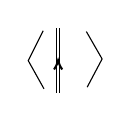
\begin{tikzpicture}[x=0.75pt,y=0.75pt,yscale=-1,xscale=1,scale=0.4, transform shape]
%uncomment if require: \path (0,410); %set diagram left start at 0, and has height of 410

%Straight Lines [id:da6679599183950475] 
\draw    (42.75,129.9) -- (42.75,52.4)(45.75,129.9) -- (45.75,52.4) ;
\draw [shift={(44.25,91.15)}, rotate = 450] [color={rgb, 255:red, 0; green, 0; blue, 0 }  ][line width=0.75]    (10.93,-4.9) .. controls (6.95,-2.3) and (3.31,-0.67) .. (0,0) .. controls (3.31,0.67) and (6.95,2.3) .. (10.93,4.9)   ;
%Straight Lines [id:da96866989164835] 
\draw    (78.25,56.4) -- (97.25,89.4) -- (79.25,123.4) ;
%Straight Lines [id:da6934326937577064] 
\draw    (26.25,55.4) -- (8.25,91.4) -- (27.25,125.4) ;
\end{tikzpicture}
                        & $i\langle G^+(\mathbf{k},\omega)\rangle$                                             \\ \hline



\tikzset{every picture/.style={line width=0.75pt}} %set default line width to 0.75pt        

\begin{tikzpicture}[x=0.75pt,y=0.75pt,yscale=-1,xscale=1,scale=0.4, transform shape]
%uncomment if require: \path (0,410); %set diagram left start at 0, and has height of 410

%Straight Lines [id:da28668922103226246] 
\draw    (505.5,288.72) -- (505.5,258.4) ;
%Shape: Ellipse [id:dp08452238525628197] 
\draw   (495.75,298.4) .. controls (495.75,293.05) and (500.12,288.72) .. (505.5,288.72) .. controls (510.88,288.72) and (515.25,293.05) .. (515.25,298.4) .. controls (515.25,303.75) and (510.88,308.08) .. (505.5,308.08) .. controls (500.12,308.08) and (495.75,303.75) .. (495.75,298.4) -- cycle ;
%Straight Lines [id:da3057641306656801] 
\draw    (505.5,338.4) -- (505.5,308.08) ;




\end{tikzpicture}
                        & $-iW_{lk}$                                                                           \\ \hline



\tikzset{every picture/.style={line width=0.75pt}} %set default line width to 0.75pt        

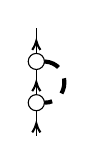
\begin{tikzpicture}[x=0.75pt,y=0.75pt,yscale=-1,xscale=1,scale=0.4, transform shape]
%uncomment if require: \path (0,410); %set diagram left start at 0, and has height of 410

%Straight Lines [id:da7079596940921928] 
\draw    (267.5,59.72) -- (267.5,29.4) ;
\draw [shift={(267.5,44.56)}, rotate = 450] [color={rgb, 255:red, 0; green, 0; blue, 0 }  ][line width=0.75]    (10.93,-4.9) .. controls (6.95,-2.3) and (3.31,-0.67) .. (0,0) .. controls (3.31,0.67) and (6.95,2.3) .. (10.93,4.9)   ;
%Shape: Ellipse [id:dp22478419986022313] 
\draw   (257.75,69.4) .. controls (257.75,64.05) and (262.12,59.72) .. (267.5,59.72) .. controls (272.88,59.72) and (277.25,64.05) .. (277.25,69.4) .. controls (277.25,74.75) and (272.88,79.08) .. (267.5,79.08) .. controls (262.12,79.08) and (257.75,74.75) .. (257.75,69.4) -- cycle ;
%Straight Lines [id:da11608178895592369] 
\draw    (267.5,109.4) -- (267.5,79.08) ;
\draw [shift={(267.5,94.24)}, rotate = 450] [color={rgb, 255:red, 0; green, 0; blue, 0 }  ][line width=0.75]    (10.93,-4.9) .. controls (6.95,-2.3) and (3.31,-0.67) .. (0,0) .. controls (3.31,0.67) and (6.95,2.3) .. (10.93,4.9)   ;

%Shape: Ellipse [id:dp33421438233375045] 
\draw   (257.75,119.08) .. controls (257.75,113.74) and (262.12,109.4) .. (267.5,109.4) .. controls (272.88,109.4) and (277.25,113.74) .. (277.25,119.08) .. controls (277.25,124.43) and (272.88,128.77) .. (267.5,128.77) .. controls (262.12,128.77) and (257.75,124.43) .. (257.75,119.08) -- cycle ;
%Straight Lines [id:da8470461387935158] 
\draw    (267.5,159.08) -- (267.5,128.77) ;
\draw [shift={(267.5,143.93)}, rotate = 450] [color={rgb, 255:red, 0; green, 0; blue, 0 }  ][line width=0.75]    (10.93,-4.9) .. controls (6.95,-2.3) and (3.31,-0.67) .. (0,0) .. controls (3.31,0.67) and (6.95,2.3) .. (10.93,4.9)   ;
%Curve Lines [id:da5905027576335966] 
\draw [line width=1.5]  [dash pattern={on 5.63pt off 4.5pt}]  (277.25,69.4) .. controls (310.25,71.4) and (308.25,119.4) .. (277.25,119.08) ;




\end{tikzpicture}
                        & factor $N/\Omega$                                                                    \\ \hline
intermediate momentum, I & $\int \frac{d^{3} l}{(2 \pi)^{3}}$                                                   \\ \hline


    \tikzset{every picture/.style={line width=0.75pt}} %set default line width to 0.75pt        

\begin{tikzpicture}[x=0.75pt,y=0.75pt,yscale=-1,xscale=1,scale=0.4, transform shape]
%uncomment if require: \path (0,410); %set diagram left start at 0, and has height of 410

%Straight Lines [id:da5008643601850559] 
\draw    (136.25,128.9) -- (136.25,51.4) ;
\draw [shift={(136.25,90.15)}, rotate = 450] [color={rgb, 255:red, 0; green, 0; blue, 0 }  ][line width=0.75]    (10.93,-4.9) .. controls (6.95,-2.3) and (3.31,-0.67) .. (0,0) .. controls (3.31,0.67) and (6.95,2.3) .. (10.93,4.9)   ;
\end{tikzpicture}
                       & $i G_{0}^{+}(\mathbf{k}, \omega)=\frac{i}{\omega-\varepsilon_{\mathrm{k}}+i \delta}$ \\ \hline
\end{tabular}
\end{table}

Let's evaluate \ref{whole-impurity-diagram-series} by assuming the most important processes are single scattering, and double scattering by the same impurity. This means that diagrams containing more than two successive scatterings off the same ion are neglected.The partial sum may easily be carried out and yields
\begin{equation}
\tikzset{every picture/.style={line width=0.75pt}} %set default line width to 0.75pt        
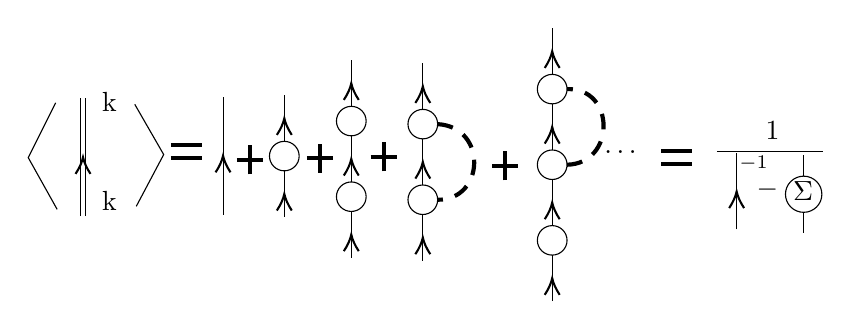
\begin{tikzpicture}[x=0.55pt,y=0.55pt,yscale=-1,xscale=1]
%uncomment if require: \path (0,410); %set diagram left start at 0, and has height of 410

%Straight Lines [id:da6679599183950475] 
\draw    (42.75,129.9) -- (42.75,52.4)(45.75,129.9) -- (45.75,52.4) ;
\draw [shift={(44.25,91.15)}, rotate = 450] [color={rgb, 255:red, 0; green, 0; blue, 0 }  ][line width=0.75]    (10.93,-4.9) .. controls (6.95,-2.3) and (3.31,-0.67) .. (0,0) .. controls (3.31,0.67) and (6.95,2.3) .. (10.93,4.9)   ;
%Straight Lines [id:da96866989164835] 
\draw    (78.25,56.4) -- (97.25,89.4) -- (79.25,123.4) ;
%Straight Lines [id:da6934326937577064] 
\draw    (26.25,55.4) -- (8.25,91.4) -- (27.25,125.4) ;
%Straight Lines [id:da3013274600825496] 
\draw [line width=1.5]    (102,83.02) -- (122.25,83.02) ;
%Straight Lines [id:da002431265709683772] 
\draw [line width=1.5]    (102,91.4) -- (122.25,91.4) ;

%Straight Lines [id:da5008643601850559] 
\draw    (136.25,128.9) -- (136.25,51.4) ;
\draw [shift={(136.25,90.15)}, rotate = 450] [color={rgb, 255:red, 0; green, 0; blue, 0 }  ][line width=0.75]    (10.93,-4.9) .. controls (6.95,-2.3) and (3.31,-0.67) .. (0,0) .. controls (3.31,0.67) and (6.95,2.3) .. (10.93,4.9)   ;
%Straight Lines [id:da6945756947603086] 
\draw    (176.5,80.72) -- (176.5,50.4) ;
\draw [shift={(176.5,65.56)}, rotate = 450] [color={rgb, 255:red, 0; green, 0; blue, 0 }  ][line width=0.75]    (10.93,-4.9) .. controls (6.95,-2.3) and (3.31,-0.67) .. (0,0) .. controls (3.31,0.67) and (6.95,2.3) .. (10.93,4.9)   ;
%Shape: Ellipse [id:dp3530646460829052] 
\draw   (166.75,90.4) .. controls (166.75,85.05) and (171.12,80.72) .. (176.5,80.72) .. controls (181.88,80.72) and (186.25,85.05) .. (186.25,90.4) .. controls (186.25,95.75) and (181.88,100.08) .. (176.5,100.08) .. controls (171.12,100.08) and (166.75,95.75) .. (166.75,90.4) -- cycle ;
%Straight Lines [id:da43208207245118435] 
\draw    (176.5,130.4) -- (176.5,100.08) ;
\draw [shift={(176.5,115.24)}, rotate = 450] [color={rgb, 255:red, 0; green, 0; blue, 0 }  ][line width=0.75]    (10.93,-4.9) .. controls (6.95,-2.3) and (3.31,-0.67) .. (0,0) .. controls (3.31,0.67) and (6.95,2.3) .. (10.93,4.9)   ;

%Straight Lines [id:da7828111751257385] 
\draw    (220.5,57.72) -- (220.5,27.4) ;
\draw [shift={(220.5,42.56)}, rotate = 450] [color={rgb, 255:red, 0; green, 0; blue, 0 }  ][line width=0.75]    (10.93,-4.9) .. controls (6.95,-2.3) and (3.31,-0.67) .. (0,0) .. controls (3.31,0.67) and (6.95,2.3) .. (10.93,4.9)   ;
%Shape: Ellipse [id:dp6295020134353576] 
\draw   (210.75,67.4) .. controls (210.75,62.05) and (215.12,57.72) .. (220.5,57.72) .. controls (225.88,57.72) and (230.25,62.05) .. (230.25,67.4) .. controls (230.25,72.75) and (225.88,77.08) .. (220.5,77.08) .. controls (215.12,77.08) and (210.75,72.75) .. (210.75,67.4) -- cycle ;
%Straight Lines [id:da5190411567838193] 
\draw    (220.5,107.4) -- (220.5,77.08) ;
\draw [shift={(220.5,92.24)}, rotate = 450] [color={rgb, 255:red, 0; green, 0; blue, 0 }  ][line width=0.75]    (10.93,-4.9) .. controls (6.95,-2.3) and (3.31,-0.67) .. (0,0) .. controls (3.31,0.67) and (6.95,2.3) .. (10.93,4.9)   ;

%Shape: Ellipse [id:dp1856254885258023] 
\draw   (210.75,117.08) .. controls (210.75,111.74) and (215.12,107.4) .. (220.5,107.4) .. controls (225.88,107.4) and (230.25,111.74) .. (230.25,117.08) .. controls (230.25,122.43) and (225.88,126.77) .. (220.5,126.77) .. controls (215.12,126.77) and (210.75,122.43) .. (210.75,117.08) -- cycle ;
%Straight Lines [id:da12064415501164083] 
\draw    (220.5,157.08) -- (220.5,126.77) ;
\draw [shift={(220.5,141.93)}, rotate = 450] [color={rgb, 255:red, 0; green, 0; blue, 0 }  ][line width=0.75]    (10.93,-4.9) .. controls (6.95,-2.3) and (3.31,-0.67) .. (0,0) .. controls (3.31,0.67) and (6.95,2.3) .. (10.93,4.9)   ;
%Straight Lines [id:da7079596940921928] 
\draw    (267.5,59.72) -- (267.5,29.4) ;
\draw [shift={(267.5,44.56)}, rotate = 450] [color={rgb, 255:red, 0; green, 0; blue, 0 }  ][line width=0.75]    (10.93,-4.9) .. controls (6.95,-2.3) and (3.31,-0.67) .. (0,0) .. controls (3.31,0.67) and (6.95,2.3) .. (10.93,4.9)   ;
%Shape: Ellipse [id:dp22478419986022313] 
\draw   (257.75,69.4) .. controls (257.75,64.05) and (262.12,59.72) .. (267.5,59.72) .. controls (272.88,59.72) and (277.25,64.05) .. (277.25,69.4) .. controls (277.25,74.75) and (272.88,79.08) .. (267.5,79.08) .. controls (262.12,79.08) and (257.75,74.75) .. (257.75,69.4) -- cycle ;
%Straight Lines [id:da11608178895592369] 
\draw    (267.5,109.4) -- (267.5,79.08) ;
\draw [shift={(267.5,94.24)}, rotate = 450] [color={rgb, 255:red, 0; green, 0; blue, 0 }  ][line width=0.75]    (10.93,-4.9) .. controls (6.95,-2.3) and (3.31,-0.67) .. (0,0) .. controls (3.31,0.67) and (6.95,2.3) .. (10.93,4.9)   ;

%Shape: Ellipse [id:dp33421438233375045] 
\draw   (257.75,119.08) .. controls (257.75,113.74) and (262.12,109.4) .. (267.5,109.4) .. controls (272.88,109.4) and (277.25,113.74) .. (277.25,119.08) .. controls (277.25,124.43) and (272.88,128.77) .. (267.5,128.77) .. controls (262.12,128.77) and (257.75,124.43) .. (257.75,119.08) -- cycle ;
%Straight Lines [id:da8470461387935158] 
\draw    (267.5,159.08) -- (267.5,128.77) ;
\draw [shift={(267.5,143.93)}, rotate = 450] [color={rgb, 255:red, 0; green, 0; blue, 0 }  ][line width=0.75]    (10.93,-4.9) .. controls (6.95,-2.3) and (3.31,-0.67) .. (0,0) .. controls (3.31,0.67) and (6.95,2.3) .. (10.93,4.9)   ;
%Straight Lines [id:da5580045724596926] 
\draw [line width=1.5]    (145.25,92.8) -- (162.25,92.8) ;
%Straight Lines [id:da21350536390327923] 
\draw [line width=1.5]    (153.75,102.4) -- (153.75,83.21) ;

%Straight Lines [id:da8624253903000908] 
\draw [line width=1.5]    (191.25,91.8) -- (208.25,91.8) ;
%Straight Lines [id:da39200924475692256] 
\draw [line width=1.5]    (199.75,101.4) -- (199.75,82.21) ;

%Straight Lines [id:da11442905940915027] 
\draw [line width=1.5]    (233.25,90.8) -- (250.25,90.8) ;
%Straight Lines [id:da6458220565812314] 
\draw [line width=1.5]    (241.75,100.4) -- (241.75,81.21) ;

%Curve Lines [id:da5905027576335966] 
\draw [line width=1.5]  [dash pattern={on 5.63pt off 4.5pt}]  (277.25,69.4) .. controls (310.25,71.4) and (308.25,119.4) .. (277.25,119.08) ;
%Straight Lines [id:da09806150660985813] 
\draw [line width=1.5]    (313.25,96.8) -- (330.25,96.8) ;
%Straight Lines [id:da8319212817021413] 
\draw [line width=1.5]    (321.75,106.4) -- (321.75,87.21) ;

%Straight Lines [id:da17267749447821656] 
\draw    (352.5,36.72) -- (352.5,6.4) ;
\draw [shift={(352.5,21.56)}, rotate = 450] [color={rgb, 255:red, 0; green, 0; blue, 0 }  ][line width=0.75]    (10.93,-4.9) .. controls (6.95,-2.3) and (3.31,-0.67) .. (0,0) .. controls (3.31,0.67) and (6.95,2.3) .. (10.93,4.9)   ;
%Shape: Ellipse [id:dp6338000815403856] 
\draw   (342.75,46.4) .. controls (342.75,41.05) and (347.12,36.72) .. (352.5,36.72) .. controls (357.88,36.72) and (362.25,41.05) .. (362.25,46.4) .. controls (362.25,51.75) and (357.88,56.08) .. (352.5,56.08) .. controls (347.12,56.08) and (342.75,51.75) .. (342.75,46.4) -- cycle ;
%Straight Lines [id:da6359368270166951] 
\draw    (352.5,86.4) -- (352.5,56.08) ;
\draw [shift={(352.5,71.24)}, rotate = 450] [color={rgb, 255:red, 0; green, 0; blue, 0 }  ][line width=0.75]    (10.93,-4.9) .. controls (6.95,-2.3) and (3.31,-0.67) .. (0,0) .. controls (3.31,0.67) and (6.95,2.3) .. (10.93,4.9)   ;

%Shape: Ellipse [id:dp8160936873445316] 
\draw   (342.75,96.08) .. controls (342.75,90.74) and (347.12,86.4) .. (352.5,86.4) .. controls (357.88,86.4) and (362.25,90.74) .. (362.25,96.08) .. controls (362.25,101.43) and (357.88,105.77) .. (352.5,105.77) .. controls (347.12,105.77) and (342.75,101.43) .. (342.75,96.08) -- cycle ;
%Straight Lines [id:da9286035597952149] 
\draw    (352.5,136.08) -- (352.5,105.77) ;
\draw [shift={(352.5,120.93)}, rotate = 450] [color={rgb, 255:red, 0; green, 0; blue, 0 }  ][line width=0.75]    (10.93,-4.9) .. controls (6.95,-2.3) and (3.31,-0.67) .. (0,0) .. controls (3.31,0.67) and (6.95,2.3) .. (10.93,4.9)   ;
%Shape: Ellipse [id:dp07506037090452533] 
\draw   (342.75,145.77) .. controls (342.75,140.42) and (347.12,136.08) .. (352.5,136.08) .. controls (357.88,136.08) and (362.25,140.42) .. (362.25,145.77) .. controls (362.25,151.12) and (357.88,155.45) .. (352.5,155.45) .. controls (347.12,155.45) and (342.75,151.12) .. (342.75,145.77) -- cycle ;
%Straight Lines [id:da3948811378599879] 
\draw    (352.5,185.77) -- (352.5,155.45) ;
\draw [shift={(352.5,170.61)}, rotate = 450] [color={rgb, 255:red, 0; green, 0; blue, 0 }  ][line width=0.75]    (10.93,-4.9) .. controls (6.95,-2.3) and (3.31,-0.67) .. (0,0) .. controls (3.31,0.67) and (6.95,2.3) .. (10.93,4.9)   ;
%Curve Lines [id:da8457780212222412] 
\draw [line width=1.5]  [dash pattern={on 5.63pt off 4.5pt}]  (362.25,96.08) .. controls (394.25,95.4) and (394.25,45.4) .. (362.25,46.4) ;
%Straight Lines [id:da17632381462435154] 
\draw [line width=1.5]    (424,87.02) -- (444.25,87.02) ;
%Straight Lines [id:da2860027932323479] 
\draw [line width=1.5]    (424,95.4) -- (444.25,95.4) ;

%Straight Lines [id:da3219886118472701] 
\draw    (473.67,138.63) -- (473.67,88.63) ;
\draw [shift={(473.67,113.63)}, rotate = 450] [color={rgb, 255:red, 0; green, 0; blue, 0 }  ][line width=0.75]    (10.93,-4.9) .. controls (6.95,-2.3) and (3.31,-0.67) .. (0,0) .. controls (3.31,0.67) and (6.95,2.3) .. (10.93,4.9)   ;
%Straight Lines [id:da7155527870457447] 
\draw    (517.71,103.59) -- (517.71,89.63) ;
%Shape: Ellipse [id:dp6470069643074525] 
\draw   (505.75,115.47) .. controls (505.75,108.91) and (511.1,103.59) .. (517.71,103.59) .. controls (524.31,103.59) and (529.67,108.91) .. (529.67,115.47) .. controls (529.67,122.03) and (524.31,127.35) .. (517.71,127.35) .. controls (511.1,127.35) and (505.75,122.03) .. (505.75,115.47) -- cycle ;
%Straight Lines [id:da765234496553557] 
\draw    (517.71,140.63) -- (517.71,127.35) ;
%Straight Lines [id:da9234724283302328] 
\draw    (460.67,87.63) -- (530.67,87.63) ;


% Text Node
\draw (55,47.02) node [anchor=north west][inner sep=0.75pt]   [align=left] {k};
% Text Node
\draw (55,112.02) node [anchor=north west][inner sep=0.75pt]   [align=left] {k};
% Text Node
\draw (385,85.02) node [anchor=north west][inner sep=0.75pt]    {$\dotsc $};
% Text Node
\draw (491,66.3) node [anchor=north west][inner sep=0.75pt]    {$1$};
% Text Node
\draw (485,104.3) node [anchor=north west][inner sep=0.75pt]    {$-$};
% Text Node
\draw (473.67,88.63) node [anchor=north west][inner sep=0.75pt]    {$^{-1}$};
% Text Node
\draw (509,105.3) node [anchor=north west][inner sep=0.75pt]    {$\Sigma $};
\end{tikzpicture}
\label{single-impurity-series}
\end{equation}
where 
\begin{center}
\tikzset{every picture/.style={line width=0.75pt}} %set default line width to 0.75pt        
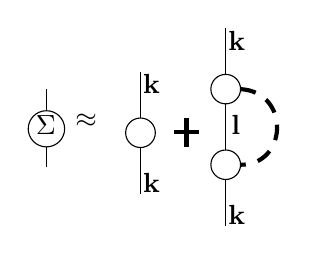
\begin{tikzpicture}[x=0.55pt,y=0.55pt,yscale=-1,xscale=1]
%uncomment if require: \path (0,410); %set diagram left start at 0, and has height of 410

%Straight Lines [id:da2478555353047407] 
\draw    (57.71,237.59) -- (57.71,223.63) ;
%Shape: Ellipse [id:dp8195879996221702] 
\draw   (45.75,249.47) .. controls (45.75,242.91) and (51.1,237.59) .. (57.71,237.59) .. controls (64.31,237.59) and (69.67,242.91) .. (69.67,249.47) .. controls (69.67,256.03) and (64.31,261.35) .. (57.71,261.35) .. controls (51.1,261.35) and (45.75,256.03) .. (45.75,249.47) -- cycle ;
%Straight Lines [id:da49340395084618693] 
\draw    (57.71,274.63) -- (57.71,261.35) ;
%Straight Lines [id:da7965677357458768] 
\draw    (119.5,242.4) -- (119.5,212.08) ;
%Shape: Ellipse [id:dp5834867502072995] 
\draw   (109.75,252.08) .. controls (109.75,246.74) and (114.12,242.4) .. (119.5,242.4) .. controls (124.88,242.4) and (129.25,246.74) .. (129.25,252.08) .. controls (129.25,257.43) and (124.88,261.77) .. (119.5,261.77) .. controls (114.12,261.77) and (109.75,257.43) .. (109.75,252.08) -- cycle ;
%Straight Lines [id:da26210627528994135] 
\draw    (119.5,292.08) -- (119.5,261.77) ;
%Straight Lines [id:da5450531939398274] 
\draw    (175.5,213.72) -- (175.5,183.4) ;
%Shape: Ellipse [id:dp7406102462871901] 
\draw   (165.75,223.4) .. controls (165.75,218.05) and (170.12,213.72) .. (175.5,213.72) .. controls (180.88,213.72) and (185.25,218.05) .. (185.25,223.4) .. controls (185.25,228.75) and (180.88,233.08) .. (175.5,233.08) .. controls (170.12,233.08) and (165.75,228.75) .. (165.75,223.4) -- cycle ;
%Straight Lines [id:da10558237608158416] 
\draw    (175.5,263.4) -- (175.5,233.08) ;
%Shape: Ellipse [id:dp052195730584338906] 
\draw   (165.75,273.08) .. controls (165.75,267.74) and (170.12,263.4) .. (175.5,263.4) .. controls (180.88,263.4) and (185.25,267.74) .. (185.25,273.08) .. controls (185.25,278.43) and (180.88,282.77) .. (175.5,282.77) .. controls (170.12,282.77) and (165.75,278.43) .. (165.75,273.08) -- cycle ;
%Straight Lines [id:da620708222735995] 
\draw    (175.5,313.08) -- (175.5,282.77) ;
%Straight Lines [id:da3887554298477651] 
\draw [line width=1.5]    (141.25,251.8) -- (158.25,251.8) ;
%Straight Lines [id:da3055944791539196] 
\draw [line width=1.5]    (149.75,261.4) -- (149.75,242.21) ;

%Curve Lines [id:da439299640958546] 
\draw [line width=1.5]  [dash pattern={on 5.63pt off 4.5pt}]  (185.25,223.4) .. controls (218.25,225.4) and (216.25,273.4) .. (185.25,273.08) ;

% Text Node
\draw (49,239.3) node [anchor=north west][inner sep=0.75pt]    {$\Sigma $};
% Text Node
\draw (119.5,212.08) node [anchor=north west][inner sep=0.75pt]   [align=left] {\textbf{k}};
% Text Node
\draw (75,238.3) node [anchor=north west][inner sep=0.75pt]    {$\approx $};
% Text Node
\draw (119.5,276.93) node [anchor=north west][inner sep=0.75pt]   [align=left] {\textbf{k}};
% Text Node
\draw (175.5,183.4) node [anchor=north west][inner sep=0.75pt]   [align=left] {\textbf{k}};
% Text Node
\draw (175.5,297.93) node [anchor=north west][inner sep=0.75pt]   [align=left] {\textbf{k}};
% Text Node
\draw (177.5,239.08) node [anchor=north west][inner sep=0.75pt]   [align=left] {\textbf{l}};
\end{tikzpicture}
\end{center}
Note that the complete series for \Circled{$\Sigma$} is
\begin{center}
\tikzset{every picture/.style={line width=0.75pt}} %set default line width to 0.75pt        
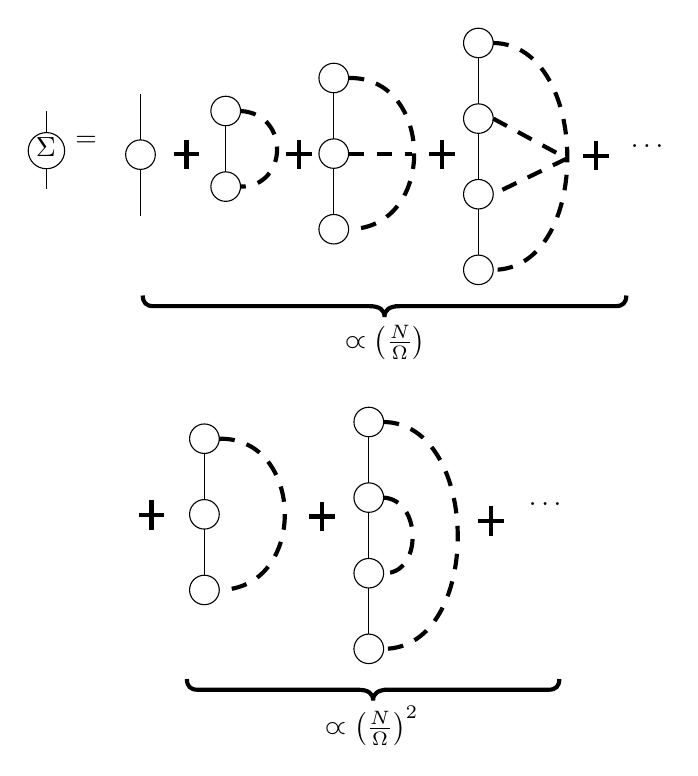
\begin{tikzpicture}[x=0.55pt,y=0.55pt,yscale=-1,xscale=1]
%uncomment if require: \path (0,705); %set diagram left start at 0, and has height of 705

%Straight Lines [id:da2478555353047407] 
\draw    (47.71,269.59) -- (47.71,255.63) ;
%Shape: Ellipse [id:dp8195879996221702] 
\draw   (35.75,281.47) .. controls (35.75,274.91) and (41.1,269.59) .. (47.71,269.59) .. controls (54.31,269.59) and (59.67,274.91) .. (59.67,281.47) .. controls (59.67,288.03) and (54.31,293.35) .. (47.71,293.35) .. controls (41.1,293.35) and (35.75,288.03) .. (35.75,281.47) -- cycle ;
%Straight Lines [id:da49340395084618693] 
\draw    (47.71,306.63) -- (47.71,293.35) ;
%Straight Lines [id:da7965677357458768] 
\draw    (109.5,274.4) -- (109.5,244.08) ;
%Shape: Ellipse [id:dp5834867502072995] 
\draw   (99.75,284.08) .. controls (99.75,278.74) and (104.12,274.4) .. (109.5,274.4) .. controls (114.88,274.4) and (119.25,278.74) .. (119.25,284.08) .. controls (119.25,289.43) and (114.88,293.77) .. (109.5,293.77) .. controls (104.12,293.77) and (99.75,289.43) .. (99.75,284.08) -- cycle ;
%Straight Lines [id:da26210627528994135] 
\draw    (109.5,324.08) -- (109.5,293.77) ;
%Shape: Ellipse [id:dp7406102462871901] 
\draw   (155.75,255.4) .. controls (155.75,250.05) and (160.12,245.72) .. (165.5,245.72) .. controls (170.88,245.72) and (175.25,250.05) .. (175.25,255.4) .. controls (175.25,260.75) and (170.88,265.08) .. (165.5,265.08) .. controls (160.12,265.08) and (155.75,260.75) .. (155.75,255.4) -- cycle ;
%Straight Lines [id:da10558237608158416] 
\draw    (165.5,295.4) -- (165.5,265.08) ;
%Shape: Ellipse [id:dp052195730584338906] 
\draw   (155.75,305.08) .. controls (155.75,299.74) and (160.12,295.4) .. (165.5,295.4) .. controls (170.88,295.4) and (175.25,299.74) .. (175.25,305.08) .. controls (175.25,310.43) and (170.88,314.77) .. (165.5,314.77) .. controls (160.12,314.77) and (155.75,310.43) .. (155.75,305.08) -- cycle ;
%Straight Lines [id:da3887554298477651] 
\draw [line width=1.5]    (131.25,283.8) -- (148.25,283.8) ;
%Straight Lines [id:da3055944791539196] 
\draw [line width=1.5]    (139.75,293.4) -- (139.75,274.21) ;

%Curve Lines [id:da439299640958546] 
\draw [line width=1.5]  [dash pattern={on 5.63pt off 4.5pt}]  (175.25,255.4) .. controls (208.25,257.4) and (206.25,305.4) .. (175.25,305.08) ;
%Shape: Ellipse [id:dp7383206567205944] 
\draw   (226.75,283.4) .. controls (226.75,278.05) and (231.12,273.72) .. (236.5,273.72) .. controls (241.88,273.72) and (246.25,278.05) .. (246.25,283.4) .. controls (246.25,288.75) and (241.88,293.08) .. (236.5,293.08) .. controls (231.12,293.08) and (226.75,288.75) .. (226.75,283.4) -- cycle ;
%Straight Lines [id:da38047468848179744] 
\draw    (236.5,323.4) -- (236.5,293.08) ;
%Shape: Ellipse [id:dp3403133897193449] 
\draw   (226.75,333.08) .. controls (226.75,327.74) and (231.12,323.4) .. (236.5,323.4) .. controls (241.88,323.4) and (246.25,327.74) .. (246.25,333.08) .. controls (246.25,338.43) and (241.88,342.77) .. (236.5,342.77) .. controls (231.12,342.77) and (226.75,338.43) .. (226.75,333.08) -- cycle ;
%Curve Lines [id:da007009060601548378] 
\draw [line width=1.5]  [dash pattern={on 5.63pt off 4.5pt}]  (246.25,233.72) .. controls (302.67,232.63) and (304.67,332.63) .. (246.25,333.08) ;
%Shape: Ellipse [id:dp35771829373861763] 
\draw   (226.75,233.72) .. controls (226.75,228.37) and (231.12,224.03) .. (236.5,224.03) .. controls (241.88,224.03) and (246.25,228.37) .. (246.25,233.72) .. controls (246.25,239.06) and (241.88,243.4) .. (236.5,243.4) .. controls (231.12,243.4) and (226.75,239.06) .. (226.75,233.72) -- cycle ;
%Straight Lines [id:da9875841078417118] 
\draw    (236.5,273.72) -- (236.5,243.4) ;
%Straight Lines [id:da7015118023288028] 
\draw [line width=1.5]  [dash pattern={on 5.63pt off 4.5pt}]  (246.25,283.4) -- (287.67,283.4) ;
%Straight Lines [id:da4960628325151931] 
\draw [line width=1.5]    (205.25,283.8) -- (222.25,283.8) ;
%Straight Lines [id:da6480371797669408] 
\draw [line width=1.5]    (213.75,293.4) -- (213.75,274.21) ;

%Shape: Ellipse [id:dp7003520544377538] 
\draw   (321.75,260.4) .. controls (321.75,255.05) and (326.12,250.72) .. (331.5,250.72) .. controls (336.88,250.72) and (341.25,255.05) .. (341.25,260.4) .. controls (341.25,265.75) and (336.88,270.08) .. (331.5,270.08) .. controls (326.12,270.08) and (321.75,265.75) .. (321.75,260.4) -- cycle ;
%Straight Lines [id:da30398624837511] 
\draw    (331.5,300.4) -- (331.5,270.08) ;
%Shape: Ellipse [id:dp0013092697739560677] 
\draw   (321.75,310.08) .. controls (321.75,304.74) and (326.12,300.4) .. (331.5,300.4) .. controls (336.88,300.4) and (341.25,304.74) .. (341.25,310.08) .. controls (341.25,315.43) and (336.88,319.77) .. (331.5,319.77) .. controls (326.12,319.77) and (321.75,315.43) .. (321.75,310.08) -- cycle ;
%Curve Lines [id:da1762989116442294] 
\draw [line width=1.5]  [dash pattern={on 5.63pt off 4.5pt}]  (341.25,210.72) .. controls (405.67,211.63) and (406.67,359.63) .. (341.25,359.77) ;
%Shape: Ellipse [id:dp0919059432356526] 
\draw   (321.75,210.72) .. controls (321.75,205.37) and (326.12,201.03) .. (331.5,201.03) .. controls (336.88,201.03) and (341.25,205.37) .. (341.25,210.72) .. controls (341.25,216.06) and (336.88,220.4) .. (331.5,220.4) .. controls (326.12,220.4) and (321.75,216.06) .. (321.75,210.72) -- cycle ;
%Straight Lines [id:da4592700821469805] 
\draw    (331.5,250.72) -- (331.5,220.4) ;
%Straight Lines [id:da4092399922684642] 
\draw [line width=1.5]  [dash pattern={on 5.63pt off 4.5pt}]  (341.25,260.4) -- (389.67,286.63) ;
%Shape: Ellipse [id:dp8221836318702264] 
\draw   (321.75,359.77) .. controls (321.75,354.42) and (326.12,350.08) .. (331.5,350.08) .. controls (336.88,350.08) and (341.25,354.42) .. (341.25,359.77) .. controls (341.25,365.12) and (336.88,369.45) .. (331.5,369.45) .. controls (326.12,369.45) and (321.75,365.12) .. (321.75,359.77) -- cycle ;
%Straight Lines [id:da7228735126740514] 
\draw    (331.5,350.08) -- (331.5,319.77) ;
%Straight Lines [id:da5303593504365808] 
\draw [line width=1.5]  [dash pattern={on 5.63pt off 4.5pt}]  (389.67,286.63) -- (341.25,310.08) ;
%Straight Lines [id:da5698850434080588] 
\draw [line width=1.5]    (299.25,283.8) -- (316.25,283.8) ;
%Straight Lines [id:da4432963135610114] 
\draw [line width=1.5]    (307.75,293.4) -- (307.75,274.21) ;

%Straight Lines [id:da2415266398742839] 
\draw [line width=1.5]    (400.25,284.8) -- (417.25,284.8) ;
%Straight Lines [id:da4340372921474619] 
\draw [line width=1.5]    (408.75,294.4) -- (408.75,275.21) ;

%Shape: Brace [id:dp6448676796499818] 
\draw  [line width=1.5]  (111,376.63) .. controls (111,381.3) and (113.33,383.63) .. (118,383.63) -- (259.83,383.63) .. controls (266.5,383.63) and (269.83,385.96) .. (269.83,390.63) .. controls (269.83,385.96) and (273.16,383.63) .. (279.83,383.63)(276.83,383.63) -- (421.67,383.63) .. controls (426.34,383.63) and (428.67,381.3) .. (428.67,376.63) ;
%Straight Lines [id:da07410677749346861] 
\draw [line width=1.5]    (108.25,520.8) -- (125.25,520.8) ;
%Straight Lines [id:da700700060848846] 
\draw [line width=1.5]    (116.75,530.4) -- (116.75,511.21) ;

%Shape: Ellipse [id:dp25309314883514067] 
\draw   (141.75,520.4) .. controls (141.75,515.05) and (146.12,510.72) .. (151.5,510.72) .. controls (156.88,510.72) and (161.25,515.05) .. (161.25,520.4) .. controls (161.25,525.75) and (156.88,530.08) .. (151.5,530.08) .. controls (146.12,530.08) and (141.75,525.75) .. (141.75,520.4) -- cycle ;
%Straight Lines [id:da15361398879570853] 
\draw    (151.5,560.4) -- (151.5,530.08) ;
%Shape: Ellipse [id:dp11922541802264952] 
\draw   (141.75,570.08) .. controls (141.75,564.74) and (146.12,560.4) .. (151.5,560.4) .. controls (156.88,560.4) and (161.25,564.74) .. (161.25,570.08) .. controls (161.25,575.43) and (156.88,579.77) .. (151.5,579.77) .. controls (146.12,579.77) and (141.75,575.43) .. (141.75,570.08) -- cycle ;
%Curve Lines [id:da6846534275233958] 
\draw [line width=1.5]  [dash pattern={on 5.63pt off 4.5pt}]  (161.25,470.72) .. controls (217.67,469.63) and (219.67,569.63) .. (161.25,570.08) ;
%Shape: Ellipse [id:dp8919508088411173] 
\draw   (141.75,470.72) .. controls (141.75,465.37) and (146.12,461.03) .. (151.5,461.03) .. controls (156.88,461.03) and (161.25,465.37) .. (161.25,470.72) .. controls (161.25,476.06) and (156.88,480.4) .. (151.5,480.4) .. controls (146.12,480.4) and (141.75,476.06) .. (141.75,470.72) -- cycle ;
%Straight Lines [id:da9808659240915968] 
\draw    (151.5,510.72) -- (151.5,480.4) ;
%Shape: Ellipse [id:dp6898707679738483] 
\draw   (249.75,509.4) .. controls (249.75,504.05) and (254.12,499.72) .. (259.5,499.72) .. controls (264.88,499.72) and (269.25,504.05) .. (269.25,509.4) .. controls (269.25,514.75) and (264.88,519.08) .. (259.5,519.08) .. controls (254.12,519.08) and (249.75,514.75) .. (249.75,509.4) -- cycle ;
%Straight Lines [id:da3999992844031298] 
\draw    (259.5,549.4) -- (259.5,519.08) ;
%Shape: Ellipse [id:dp4709695539942117] 
\draw   (249.75,559.08) .. controls (249.75,553.74) and (254.12,549.4) .. (259.5,549.4) .. controls (264.88,549.4) and (269.25,553.74) .. (269.25,559.08) .. controls (269.25,564.43) and (264.88,568.77) .. (259.5,568.77) .. controls (254.12,568.77) and (249.75,564.43) .. (249.75,559.08) -- cycle ;
%Curve Lines [id:da940049566421093] 
\draw [line width=1.5]  [dash pattern={on 5.63pt off 4.5pt}]  (269.25,459.72) .. controls (333.67,460.63) and (334.67,608.63) .. (269.25,608.77) ;
%Shape: Ellipse [id:dp6253341496158781] 
\draw   (249.75,459.72) .. controls (249.75,454.37) and (254.12,450.03) .. (259.5,450.03) .. controls (264.88,450.03) and (269.25,454.37) .. (269.25,459.72) .. controls (269.25,465.06) and (264.88,469.4) .. (259.5,469.4) .. controls (254.12,469.4) and (249.75,465.06) .. (249.75,459.72) -- cycle ;
%Straight Lines [id:da8751810296393059] 
\draw    (259.5,499.72) -- (259.5,469.4) ;
%Shape: Ellipse [id:dp8407456531271822] 
\draw   (249.75,608.77) .. controls (249.75,603.42) and (254.12,599.08) .. (259.5,599.08) .. controls (264.88,599.08) and (269.25,603.42) .. (269.25,608.77) .. controls (269.25,614.12) and (264.88,618.45) .. (259.5,618.45) .. controls (254.12,618.45) and (249.75,614.12) .. (249.75,608.77) -- cycle ;
%Straight Lines [id:da14298245758103656] 
\draw    (259.5,599.08) -- (259.5,568.77) ;
%Straight Lines [id:da6036254548506781] 
\draw [line width=1.5]    (220.25,521.8) -- (237.25,521.8) ;
%Straight Lines [id:da28515530631102337] 
\draw [line width=1.5]    (228.75,531.4) -- (228.75,512.21) ;

%Curve Lines [id:da2089293006978581] 
\draw [line width=1.5]  [dash pattern={on 5.63pt off 4.5pt}]  (269.25,509.4) .. controls (294.67,510.97) and (294.67,559.97) .. (269.25,559.08) ;
%Straight Lines [id:da7741500484806249] 
\draw [line width=1.5]    (331.25,524.8) -- (348.25,524.8) ;
%Straight Lines [id:da7102780089195931] 
\draw [line width=1.5]    (339.75,534.4) -- (339.75,515.21) ;

%Shape: Brace [id:dp23003029551106846] 
\draw  [line width=1.5]  (140,628.63) .. controls (140,633.3) and (142.33,635.63) .. (147,635.63) -- (252.33,635.63) .. controls (259,635.63) and (262.33,637.96) .. (262.33,642.63) .. controls (262.33,637.96) and (265.66,635.63) .. (272.33,635.63)(269.33,635.63) -- (377.67,635.63) .. controls (382.34,635.63) and (384.67,633.3) .. (384.67,628.63) ;

% Text Node
\draw (39,271.3) node [anchor=north west][inner sep=0.75pt]    {$\Sigma $};
% Text Node
\draw (65,270.3) node [anchor=north west][inner sep=0.75pt]    {$=$};
% Text Node
\draw (430,276.02) node [anchor=north west][inner sep=0.75pt]    {$\dotsc $};
% Text Node
\draw (242,394.63) node [anchor=north west][inner sep=0.75pt]    {$\varpropto \left(\frac{N}{\Omega }\right)$};
% Text Node
\draw (363,511.02) node [anchor=north west][inner sep=0.75pt]    {$\dotsc $};
% Text Node
\draw (229,644.63) node [anchor=north west][inner sep=0.75pt]    {$\varpropto \left(\frac{N}{\Omega }\right)^{2}$};


\end{tikzpicture}
\end{center}
For small $N/\Omega$, we only consider the terms $\varpropto(N/\Omega)$, i.e., terms representing multiple scattering from a single impurity. Translating (\ref{single-impurity-series}) into functions
\begin{equation}\langle G(\mathbf{k}, \omega)\rangle=1 /\left[\omega-\epsilon_{k}+i \delta-\Sigma(\mathbf{k}, \omega)\right]
\label{single-impurity-G}
\end{equation}
where
\begin{equation}\Sigma(\mathbf{k}, \omega)=\frac{N}{\Omega} W_{\mathbf{k} \mathbf{k}}+\frac{N}{\Omega} \int \frac{d^{3} \mathbf{l}}{(\mathbf{2} \pi)^{3}} \frac{\left|W_{k l}\right|^{2}}{\omega-\epsilon_{l}+i \delta}
\label{single-impurity-sigma}
\end{equation}
In order to find the new energy and lifetime of the electron, we need the complex pole of (\ref{single-impurity-G}), that is:
\begin{equation}\omega-\epsilon_{k}-\Sigma(\mathbf{k}, \omega)+i \delta=0
\label{inplace-370}
\end{equation}
\redp{Note: if in \ref{single-impurity-G} we use the original sum over $\mathbf{l}$,$\Sigma_{\mathbf{l}}$ instead of $\int d^3\mathbf{l}$, we find that, the pole equation \ref{single-impurity-sigma} will have real solutions. This can be seen at once by plotting $(N / \Omega) W_{\mathbf{k} \mathbf{k}}+(N / \Omega) \sum_{\mathbf{t}}\left|W_{\mathbf{kl}}\right|^{2} /\left(\omega-\epsilon_{\mathbf{l}}+i \delta\right)$ and $y(\mathbf{k}, \omega)=\omega-\epsilon_{\mathbf{k}} \mathbf{v} s . \omega$ and noting that the poles occur at the intersection of $\Sigma(k,\omega)$ and $y(\mathbf{k},\omega)$.\textbf{The complex solution of \ref{inplace-370}} arise because we have gone from a sum to an integral.} 

\begin{imp}
If $W$ is small so that $\Sigma$ is small then the zeroth-order approximation to $\omega$ is $\omega=\epsilon_{\mathbf{k}}$. 

The first-order approximation may be obtained by setting $\omega=\epsilon_k$ into $\Sigma(\mathbf{k},\omega)$ and re-solving for $\omega$. TO do this, we imagine $\delta$ is finite to start with, then take the limit $\delta\rightarrow0$. Multiplying numerator and denominator of the integrand of $\Sigma$ by $\omega-\epsilon_{\mathbf{l}}-i\delta$ we find for the real and imaginary parts of $\Sigma(\mathbf{k},\epsilon_{k})$:
\begin{equation}\begin{aligned}
\operatorname{Re} \sum\left(\mathbf{k}, \epsilon_{k}\right) &=\frac{N}{\Omega} W_{k k}+\lim _{\delta \rightarrow 0}\left(\frac{N}{\Omega}\right) \int \frac{d^{3} \mathbf{l}}{(2 \pi)^{3}} \frac{\left|W_{l k}\right|^{2}\left(\epsilon_{k}-\epsilon_{l}\right)}{\left(\epsilon_{k}-\epsilon_{l}\right)^{2}+\delta^{2}} \\
&=\frac{N}{\Omega} W_{k k}+\left(\frac{N}{\Omega}\right) P\left( \int \frac{d^{3} \mathbf{l}}{(2 \pi)^{3}} \frac{\left|W_{l k}\right|^{2}}{\left(\epsilon_{k}-\epsilon_{l}\right)}\right)
\end{aligned}
\label{real-sigma}
\end{equation}
\begin{equation}\begin{aligned}
\operatorname{Im} \sum\left(\mathbf{k}, \epsilon_{k}\right) &=-\lim _{\delta \rightarrow 0}\left(\frac{N}{\Omega}\right) \int \frac{d^{3} \mathbf{l}}{(2 \pi)^{3}}\left|W_{kl}\right|^{2} \frac{\delta}{\left(\epsilon_{k}-\epsilon_{l}\right)^{2}+\delta^{2}} \\
&=-\pi\left(\frac{N}{\Omega}\right) \int \frac{d^{3} \mathbf{l}}{(2 \pi)^{3}}\left|W_{kl}\right|^{2} \delta\left(\epsilon_{k}-\epsilon_{l}\right)
\end{aligned}
\label{imaginary-sigma}
\end{equation}
\end{imp}
\bluep{Where $P$ stands for "principal part"}. Using the usual definition, we have the following example of "principal part":
$$P \left(\int_{-a}^{+b} \frac{d x}{x}\right)=\lim _{\delta \rightarrow 0}\left\{\int_{-\delta}^{-b} \frac{d x}{x}+\int_{+\delta}^{+b} \frac{d x}{x}\right\}=\lim _{\delta \rightarrow 0}\{\ln (-\delta)-\ln (-a)+\ln b-\ln \delta\}=\ln b / a$$
or using the alternative definition:
$$P (\int_{-a}^{+b} \frac{d x}{x})=\lim _{\delta \rightarrow 0} \int_{-a}^{+b} d x \frac{x}{x^{2}+\delta^{2}}=\lim _{\delta \rightarrow 0} \frac{1}{2} \int_{-a}^{+b} \frac{d\left(x^{2}\right)}{x^{2}+\delta^{2}}=\left.\lim _{\delta \rightarrow 0} \frac{1}{2} \ln \left(x^{2}+\delta^{2}\right)\right|_{-a} ^{b}=\ln b / a$$
\begin{equation}\begin{aligned}
\operatorname{Im} \sum\left(\mathbf{k}, \epsilon_{k}\right) &=-\lim _{\delta \rightarrow 0}\left(\frac{N}{\Omega}\right) \int \frac{d^{3} \mathbf{l}}{(2 \pi)^{3}}\left|W_{\mathbf{lk}}\right|^{2} \frac{\delta}{\left(\epsilon_{\mathbf{k}}-\epsilon_{l}\right)^{2}+\delta^{2}} \\
&=-\pi\left(\frac{N}{\Omega}\right) \int \frac{d^{3} \mathbf{l}}{(2 \pi)^{3}}\left|W_{\mathbf{lk}}\right|^{2} \delta\left(\epsilon_{\mathbf{k}}-\epsilon_{l}\right)
\end{aligned}\end{equation}
In \ref{imaginary-sigma} we used the \redp{"squeezed Lorentzian"} definition of $\delta$-function. The results of \ref{real-sigma} and \ref{imaginary-sigma} are usually obtained with the following theorem:
\begin{imp}
\begin{equation}\frac{1}{x+i \delta}=P (\frac{1}{x})-i \pi \delta(x)\end{equation}
which is short for 
\begin{equation}\int \frac{d x f(x)}{x+i \delta}=P \int \frac{d x f(x)}{x}-i \pi \int d x f(x) \delta(x)
\label{well-known-complex-function-theorem}
\end{equation}
\end{imp}
This can be applied in the present case by noting that the integral in $\Sigma(\mathbf{k},\omega)$ may be written in the general form:
\begin{equation}\int d^{3} \mathbf{l} \frac{\boldsymbol{A}(\mathbf{l}, \ldots)}{\boldsymbol{B}(\mathbf{l}, \ldots)+i \boldsymbol{\delta}}=\int d \phi \int d \boldsymbol{\theta} \sin \theta \int d l  \frac{l^{2}A(l, \boldsymbol{\theta}, \phi, \ldots)}{B(l, \boldsymbol{\theta}, \boldsymbol{\phi}, \ldots)+i \delta}\end{equation}
Only the $\mathbf{l}$-variable is relevant here. If we let $x=B(l)$ so $l=B^{-1}(x)$ then $\int d l$ may be written in terms of $x$ using (\ref{well-known-complex-function-theorem}).(\bluep{$f(x)=l^2B^{\prime,-1}(x)A$}). Transforming back to $\mathbf{l}$ again after this is done yields
$$\int d^{3} \mathbf{l} \frac{A(\mathbf{l}, \ldots)}{B(\mathbf{l}, \ldots)+i \delta}=P \int d^{3} \mathbf{l} \frac{A(\mathbf{l}, \ldots)}{B(\mathbf{l}, \ldots)}-i \pi \int d^{3} \mathbf{l} A(\mathbf{l}, \ldots) \delta[B(\mathbf{l}, \ldots)]$$
Hence, using (\ref{real-sigma},\ref{imaginary-sigma}) we find
\begin{equation}\epsilon_{k}^{\prime}=\epsilon_{k}+\frac{N}{\Omega} W_{k k}+\left(\frac{N}{\Omega}\right) P \int \frac{d^{3} \mathbf{l}}{(2 \pi)^{3}} \frac{\left|W_{l k}\right|^{2}}{\epsilon_{k}-\epsilon_{l}}\end{equation}
\begin{equation}\tau_{k}^{-1}=\pi\left(\frac{N}{\Omega}\right) \int \frac{d^{3} \mathbf{l}}{(2 \pi)^{3}}\left|W_{l k}\right|^{2} \delta\left(\epsilon_{k}-\epsilon_{l}\right)\end{equation}
\newpage
\section{Quantum Particle in Fermi System}
\subsection{Propagator method in many-body systems}
In this chapter we will start with non-interacting Fermi-system problem. This is really a fake many-body problem,since as the problem is actually only a one-body problem. By doing this trivial problem, we will describe Fermi system very simply in terms of a few particles above the Fermi level, and a few removed particles, or "holes" below. Second, it allows us to introduce the language of the many-body problem,"\bluep{occupation number formalism}", or "\bluep{second quantization}". Finally, it shows us how to extend the definition of the propagator to the case where $t_2<t_1$. In this case, \textbf{the Green's function turns out to describe the propagation of removed particles, or "holes", which are represented diagrammatically by a downward-going arrow.}

By introducing a tree-level two-body interaction 
\begin{center}
\tikzset{every picture/.style={line width=0.75pt}} %set default line width to 0.75pt        

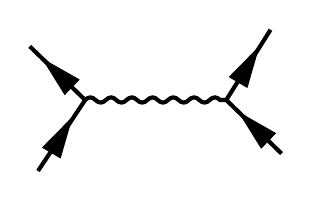
\begin{tikzpicture}[x=0.75pt,y=0.75pt,yscale=-1,xscale=1]
%uncomment if require: \path (0,705); %set diagram left start at 0, and has height of 705

%Straight Lines [id:da613823184290475] 
\draw [line width=1.5]    (491.42,548.13) .. controls (493.09,546.46) and (494.75,546.46) .. (496.42,548.13) .. controls (498.09,549.8) and (499.75,549.8) .. (501.42,548.13) .. controls (503.09,546.46) and (504.75,546.46) .. (506.42,548.13) .. controls (508.09,549.8) and (509.75,549.8) .. (511.42,548.13) .. controls (513.09,546.46) and (514.75,546.46) .. (516.42,548.13) .. controls (518.09,549.8) and (519.75,549.8) .. (521.42,548.13) .. controls (523.09,546.46) and (524.75,546.46) .. (526.42,548.13) .. controls (528.09,549.8) and (529.75,549.8) .. (531.42,548.13) .. controls (533.09,546.46) and (534.75,546.46) .. (536.42,548.13) .. controls (538.09,549.8) and (539.75,549.8) .. (541.42,548.13) .. controls (543.09,546.46) and (544.75,546.46) .. (546.42,548.13) .. controls (548.09,549.8) and (549.75,549.8) .. (551.42,548.13) .. controls (553.09,546.46) and (554.75,546.46) .. (556.42,548.13) -- (559.42,548.13) -- (559.42,548.13) ;
%Straight Lines [id:da6353755682299548] 
\draw [line width=1.5]    (464.75,522.3) -- (491.42,548.13) ;
%Straight Lines [id:da6254606220772768] 
\draw [line width=1.5]    (559.42,548.13) -- (586.08,573.97) ;
%Straight Lines [id:da5480869883300985] 
\draw [line width=1.5]    (491.42,548.13) -- (468.75,582.3) ;
%Straight Lines [id:da49445752084181116] 
\draw [line width=1.5]    (580.75,514.3) -- (559.42,548.13) ;
%Shape: Triangle [id:dp022384072825595847] 
\draw  [fill={rgb, 255:red, 0; green, 0; blue, 0 }  ,fill opacity=1 ] (471.18,528.57) -- (488.37,538.35) -- (481.61,545.37) -- cycle ;
%Shape: Triangle [id:dp5669679661948073] 
\draw  [fill={rgb, 255:red, 0; green, 0; blue, 0 }  ,fill opacity=1 ] (565.84,554.41) -- (583.04,564.18) -- (576.28,571.21) -- cycle ;
%Shape: Triangle [id:dp23872151900315752] 
\draw  [fill={rgb, 255:red, 0; green, 0; blue, 0 }  ,fill opacity=1 ] (574.92,522.94) -- (569.46,541.95) -- (561.04,537.03) -- cycle ;
%Shape: Triangle [id:dp5504301680867448] 
\draw  [fill={rgb, 255:red, 0; green, 0; blue, 0 }  ,fill opacity=1 ] (484.92,556.94) -- (479.46,575.95) -- (471.04,571.03) -- cycle ;




\end{tikzpicture}
\end{center}
we again can represent the propagator for this case as an infinite series of diagrams, which may be evaluated approximately by partial summation.

\bluep{The Hartree and Hartree-Fock are the crudest of the approximations and yield quasi particles with infinite lifetimes. The RPA yields the energy and lifetime of quasi particles in a high-density electron gas, while the ladder approxiamation is good for low-density systems like nuclear matter. Only the Hartree and Hartree-Fock will be discussed in this chapter.}
\begin{table}[H]
        \centering
        \caption{Some important partial sum approx.}
\begin{tabular}{|p{0.45\textwidth}|p{0.33\textwidth}|}
\hline 
 \begin{center}
{\fontfamily{helvet}\selectfont Types of diagrams summed over}
\end{center}
 & \begin{center}
{\fontfamily{helvet}\selectfont Name of approximation}
\end{center}
 \\
\hline 
 \begin{center}
{\fontfamily{helvet}\selectfont Bubbles}
\end{center}
 & \begin{center}
{\fontfamily{helvet}\selectfont Hartree}
\end{center}
 \\
\hline 
 \begin{center}
{\fontfamily{helvet}\selectfont Bubbles and open oysters}
\end{center}
 & \begin{center}
{\fontfamily{helvet}\selectfont Hartree-Fock}
\end{center}
 \\
\hline 
 \begin{center}
{\fontfamily{helvet}\selectfont Rings}
\end{center}
 & \begin{center}
{\fontfamily{helvet}\selectfont Random phase approx(RPA)}
\end{center}
 \\
\hline 
 \begin{center}
{\fontfamily{helvet}\selectfont Ladders}
\end{center}
 & \begin{center}
{\fontfamily{helvet}\selectfont Ladder approximation}
\end{center}
 \\
 \hline
\end{tabular}
        \end{table}
\subsection{Non-interacting Fermi system in external potential: particle- hole picture}
We first introduce the particle-hole nomenclature for describing Fermi systems. Suppose we have a single particle in a potential $U(\mathbf{r})$, with energy eigenstates $\phi_k(\mathbf{r})$. The energy levels may be represented as in Fig.\ref{fig:non-interacting-fermi},where for simplicity the system is non-degenerate.
\begin{figure}[H]
    \centering
    \includegraphics[scale=0.6]{screenshots/particle-hole.PNG}
    \caption{Non-interacting Fermi System}
    \label{fig:non-interacting-fermi}
\end{figure}
In the case where $U(\mathbf{r})=0$, the particles are free and $\mathbf{k}$ in \ref{fig:non-interacting-fermi}(a) are momentum, or wavenumber. The ground state of the single particle has energy $\epsilon_F$. If we now put N particles into the system, by Pauli principle the energy levels will be filled from the bottom as shown in \ref{fig:non-interacting-fermi}(a) for $N=5$. The highest filled energy level is the \textit{\textbf{Fermi level}},$\epsilon_F$. In ground state, the free particles fill a sphere in $\mathbf{k}-$space having radius $k_F=\sqrt{2m\epsilon_F}$,where $k_F$ is called the \textbf{Fermi momentum}. The filled sphere is called Fermi sea. The surface of this sphere is \textbf{Fermi surface}.

In Fig \ref{fig:non-interacting-fermi}(b) the excited states of the system are formed by removing a particle from a state below $\epsilon_F$ to a state above. The empty state here is called "hole". In "\bluep{particle-hole description}" we can omit the filled Fermi sea and only focus on excited particle and holes, yielding \ref{fig:non-interacting-fermi}(c) and (d). \textbf{\redp{Since a hole in state $\phi_k$ is actually removal of a particle from the system, the hole represents energy $\epsilon_k$ removed. Hence the hole energy is}}
\begin{equation}\epsilon_{k}^{\text {hole }}=-\epsilon_{k}\end{equation}
The time-dependent wave function is thus
\begin{equation}\psi_{k}(t)^{\text {hole }}=\phi_{k} e^{-i\left(-\epsilon_{k}\right) t}, \quad \epsilon_{k}<\epsilon_{F}\end{equation}
\subsection{A primer of second quantization formalism}
The total wave function for the ground and excited states of a system of non-interacting particles is the Slater determinant:
\begin{equation}\Phi_{k_{1}, \ldots, k_{N}}\left(\mathbf{r}_{1}, \ldots, \mathbf{r}_{N}\right)=\frac{1}{\sqrt{(N !)}}\left|\begin{array}{cc}
\phi_{k_{1}}\left(\mathbf{r}_{1}\right) \ldots \phi_{k_{1}}\left(\mathbf{r}_{N}\right) \\
\vdots & \vdots \\
\phi_{k_{N}}\left(\mathbf{r}_{1}\right) \ldots \phi_{k_{N}}\left(\mathbf{r}_{N}\right)
\end{array}\right|
\label{slater-determinant}
\end{equation}
\textbf{If the particles are allowed to interact with each other or external potential,} then the exact wave function of the system is a linear combination of \ref{slater-determinant}:
\begin{equation}\Psi\left(\mathbf{r}_{1}, \ldots, \mathbf{r}_{N}\right)=\sum_{k_{1}, \ldots, k_{N}} A_{k_{1}, \ldots, k_{N}} \Phi_{k_{1}, \ldots, k_{N}}\left(\mathbf{r}_{1}, \ldots, \mathbf{r}_{N}\right)\end{equation}
That is, the $\Phi_{k_1,k_2,\ldots}$ for the non-interacting system are the basis states used to describe the interacting system. Noting that all particles are indistinguishable, the essential information in \ref{slater-determinant} is just how many particles in each state, $n$. For short, we shall represent this as
\begin{equation}
    \Phi_{k_1,k_2,\ldots}=\left|n_{p_1},n_{p_2},\ldots\right\rangle
\label{linear-comb-occ-vec}
\end{equation}
meaning:$n_{p_{1}}$ particles in state $\phi_{p_{1}}, n_{p_{2}}$ in $\phi_{p_{3}},$ etc., where $n=0$ or 1 by Pauli principle. This notation is called "\redp{occupation number notation}". It is important to note that just as the original Slater determinant form a complete orthogonal set of basis functions, so do the states in occupation number notation and we have
\begin{equation}\left\langle n_{1}^{\prime}, \ldots n_{i}^{\prime} \ldots | n_{1}, \ldots, n_{i} \ldots\right\rangle=\delta_{n_1^{\prime}n_1}\ldots\delta_{n_i^{\prime}n_i}\ldots
\end{equation}
The wave function for interacting system is now becoming:
\begin{equation}\Psi=\sum_{n_{1}, \ldots, n_{i}, \ldots} A_{n_{1}, \ldots, n_{i}, \ldots}\left|n_{1}, \ldots, n_{i}, \ldots\right\rangle\end{equation}
In the particle-hole notation, it is necessary to introduce hole creation and destruction operators, $b_1^{\dagger}, b_{1}$, and similarly particle operators $a_1^{\dagger}, a_{1},$ as follows:
if $k_{i}<k_{F},$ then $c_{i}$ destroys a particle under the Fermi level, thus creating a hole. Hence
\begin{equation}\begin{aligned}
\text { for } k_{l}>k_{F}, & c_{l}=a_{l} \\
k_{l}<k_{F}, & c_{l}=b^{\dagger}_l
\end{aligned}\end{equation}
and
\begin{equation}\begin{aligned}
\text { for } k_{l}>k_{F}, & c_{l}^{\dagger}=a_{l}^{\dagger} \\
k_{l}<k_{F}, & c_{l}^{\dagger}=b_{l}
\end{aligned}\end{equation}
Simple examples of how the particle-hole operators work are:
$$a_{i}^{\dagger}|0\rangle=\left|1_i^{p}\right\rangle, \quad a_{i}\left|1_l^{p}\right\rangle=\delta_{il}|0\rangle, \quad b_{j}^{\dagger} a_{i}^{\dagger}\left|1_{m}^{\rho}\right\rangle=\left|1_{m}^{p}, 1_i^{p}, 1_j^{h}\right\rangle$$
where the superscripts represent "particle" and "hole", respectively. \redp{The operator in the occupation number formalism, $\mathcal{O}^{occ}$ is:}
\begin{equation}\mathcal{O}^{occ}=\sum_{m n} \mathcal{O}_{m n} c_{m}^{\dagger} c_{n}\end{equation}
where
\begin{equation}\begin{array}{l}
c_{l}=\theta_{k_{l}-k_{F}} a_{l}+\theta_{k_{F-k_{l}}} b_{l}^{\dagger} \\
c_{l}^{\dagger}=\theta_{k_{1}-k_{F}} a_{l}^{\dagger}+\theta_{k_{F}-k_{l}} b_{l}
\end{array}\end{equation}
and $\theta_{x}=1$ for $x>0 ; \quad \theta_{x}=0$ for $x<0$.

The Hamiltonian for an arbitrary system may be expressed in occupation number or particle-hole formalism. Suppose the system Hamiltonian in old Neanderthal notation describes a system in an external perturbing potential:
\begin{equation}H_{\text {Neand. }}=\underbrace{\sum_{i}\left[\frac{p_{1}^{2}}{2 m}+U\left(\mathbf{r}_{i}\right)\right]}_{H_{0}}+\underbrace{\sum_{i} V\left(\mathbf{r}_{i}\right)}_{H_{1}(\text { perturbation })}\end{equation}
The single-particle states $\phi_k$ satisfy:
\begin{equation}\left[\frac{p^{2}}{2 m}+U(\mathbf{r})\right] \phi_{k}=\epsilon_{k} \phi_{k}\end{equation}
Then it is found that
\begin{equation}H_{0}=\sum_{k} \epsilon_{k} c^{\dagger}_{k} c_{k}=\sum_{k>k_{F}} \epsilon_{k} a_{k}^{\dagger} a_{k}+\sum_{k<k_{F}} \epsilon_{k} b_{k} b^{\dagger}_{k}
\label{H0-Nead}
\end{equation}
\begin{equation}\begin{aligned}
H_{1}=& \sum_{m, n>k_{F}} V_{m n} a_{m}^{\dagger} a_{n}+\sum_{m>k_{F},n<k_F} V_{m n} a_{m}^{\dagger} b_{n}^{\dagger}+\sum_{m<k_{F}, n>k_{F}} V_{m n} b_{m} a_{n}+\\
&+\sum_{m, n<k_{F}} V_{m n} b_{m} b_{n}^{\dagger}
\end{aligned}
\label{H1}
\end{equation}
For a system of mutually interacting particles with a Hamiltonian
\begin{equation}H_{\mathrm{old}}=\underbrace{\sum_{l} \frac{p_{l}^{2}}{2 m}}_{H_{0}}+\frac{1}{2} \underbrace{\sum_{i, J} V\left(\mathbf{r}_{i}-\mathbf{r}_{j}\right)}_{H_{1}(\text { perturbation })}
\label{mutual-interact-hamiltonian}
\end{equation}
We also find that
\begin{equation}H_{0}=\sum_{k>k_{F}} \epsilon_{k} a_{k}^{\dagger} a_{k}+\sum_{k<k_{F}} \epsilon_{k} b_{k} b^{\dagger}_{k}\quad\epsilon_k=k^2/2m\end{equation}
\begin{equation}\begin{aligned}
H_{1}&=\frac{1}{2} \sum_{k, l, m, n>k_{F}} V_{k l m n} a_{l}^{\dagger} a_{k}^{\dagger} a_{m} a_{n}+\sum_{k, l, m>k_{F};n<k_F} V_{k l m n} a_{l}^{\dagger} a^{\dagger}_{k} a_{m} b_{n}^{\dagger}+\\
&+\cdots+\frac{1}{2} \sum_{k, l, m, n<k_{r}} V_{k l m n} b_{l} b_{k} b_{m}^{\dagger} b_{n}^{\dagger}
\end{aligned}
\label{mutual-interact-H1}
\end{equation}
We will define $V_{klmn}$ later. It should be carefully remembered that \textbf{\bluep{in the case of interacting system, the wave functions  are given by the linear combination of \ref{linear-comb-occ-vec}.}}

\subsection{Propagator for non-interacting Fermi system in external perturbing potential}
To treat the general situation of "holes", we extend the definition of propagator to times $t_2<t_1$. This leads us to the definition:
\begin{imp}
\begin{equation}
    iG(k_2,k_1,t_2-t_1)_{t_2<t_1}\equiv i G^{-}\left(k_{2}, k_{1}, t_{2}-t_{1}\right)
\end{equation}
which is $-1\times$probability amplitude that if at time $t_{2}$ we remove a particle in state $\phi_{k_{2}}$ from (i.e., if we add a hole in $\phi_{k_{2}}$ to) the interacting system in its ground state, then at time $t_{1}$ the system will be in its ground state with a particle removed from (i.e., an added hole in $) \phi_{k_{1}}$.\bluep{ The factor of (-1) here compared with $iG^+$ comes because we have fermions. Note that $G^-$ is called an "advanced" propagator or Green's function.}
\end{imp}
\redp{for $\left.t_{2}>t_{1} \text { (but not for } t_{2}=t_{1} !\right), G^{-}$ is defined so that}
\begin{equation}i G^{-}\left(k_{2}, k_{1}, t_{2}-t_{1}\right)_{t_{2}>r_{1}}=0\end{equation}

In the case of a free hole, we have
\begin{equation}G_{0}^{-}\left(k, t_{2}-t_{1}\right)=\left\{\begin{array}{l}
i \theta_{t_{1}-t_{2}} e^{-i \epsilon_{k}\left(t_{2}-t_{1}\right)}\quad t_2\neq t1,\epsilon_k<\epsilon_F \\
i, \quad \text { for } t_{2}=t_{1}
\end{array}\right.
\label{Gminus-t-space}
\end{equation}
with Fourier transform
\begin{equation}G_{0}^{-}(k, \omega)=\frac{1}{\omega-\epsilon_{k}-i \delta}, \quad \epsilon_{k}<\epsilon_{F}
\label{Gminus-k-space}
\end{equation}
The interaction amplitude, $V_{kl}$, merits some discussion. It is given by 
\begin{equation}V_{k l}=\int d^{3} \mathbf{r} \phi_{k}^{*}(\mathbf{r}) V(\mathbf{r}, \mathbf{p}) \phi_{l}(\mathbf{r})
\label{Vkl}
\end{equation}
There are four possibilities of $V_{kl}$ shown in the table below. They mean:(a) scattering of a particle in particle-hole formalism from state $\phi_{l}$ to $\phi_{k},$ (b) the potential scatters a particle out of state $\phi_{l},$ where $\epsilon_{l}<\epsilon_{F},$ into state $\phi_{k}, \epsilon_{k}>\epsilon_{F},$ thus simultaneously creating a particle in $\phi_{k}$ and a hole in $\phi_{l},(c),$ etc. \redp{Note that these four possibilities correspond to the four interaction terms in the particle-hole Hamiltonian for this case (\ref{mutual-interact-hamiltonian})}.
\begin{figure}[H]
    \centering
\tikzset{every picture/.style={line width=0.75pt}} %set default line width to 0.75pt        
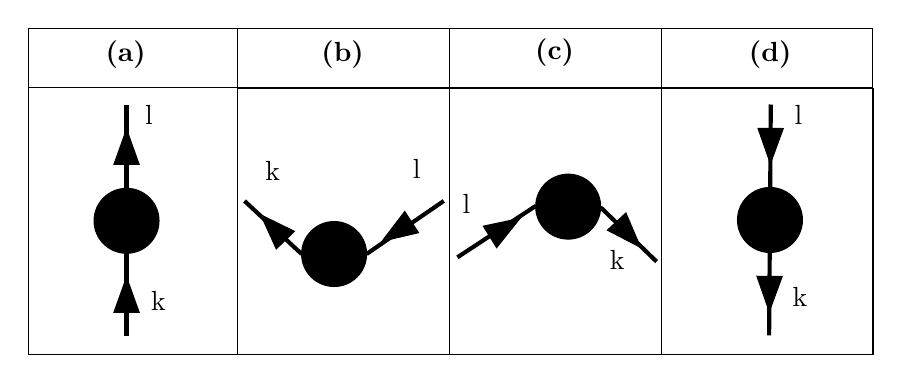
\begin{tikzpicture}[x=0.75pt,y=0.75pt,yscale=-1,xscale=1]
%uncomment if require: \path (0,244); %set diagram left start at 0, and has height of 244

%Shape: Circle [id:dp7355643708429443] 
\draw  [fill={rgb, 255:red, 0; green, 0; blue, 0 }  ,fill opacity=1 ] (147.73,133.97) .. controls (147.73,125.33) and (154.73,118.33) .. (163.37,118.33) .. controls (172,118.33) and (179,125.33) .. (179,133.97) .. controls (179,142.6) and (172,149.6) .. (163.37,149.6) .. controls (154.73,149.6) and (147.73,142.6) .. (147.73,133.97) -- cycle ;
%Straight Lines [id:da3859042750603179] 
\draw [line width=1.5]    (163.37,149.6) -- (163.37,189.6) ;
%Straight Lines [id:da7654556741518936] 
\draw [line width=1.5]    (163.37,78.33) -- (163.37,118.33) ;
%Shape: Triangle [id:dp19291169740752956] 
\draw  [fill={rgb, 255:red, 0; green, 0; blue, 0 }  ,fill opacity=1 ] (163.37,89.87) -- (169.43,106.79) -- (157.3,106.79) -- cycle ;
%Shape: Triangle [id:dp3466064725515261] 
\draw  [fill={rgb, 255:red, 0; green, 0; blue, 0 }  ,fill opacity=1 ] (163.37,161.14) -- (169.43,178.06) -- (157.3,178.06) -- cycle ;
%Shape: Circle [id:dp605096323889595] 
\draw  [fill={rgb, 255:red, 0; green, 0; blue, 0 }  ,fill opacity=1 ] (247.73,149.97) .. controls (247.73,141.33) and (254.73,134.33) .. (263.37,134.33) .. controls (272,134.33) and (279,141.33) .. (279,149.97) .. controls (279,158.6) and (272,165.6) .. (263.37,165.6) .. controls (254.73,165.6) and (247.73,158.6) .. (247.73,149.97) -- cycle ;
%Straight Lines [id:da59504555135735] 
\draw [line width=1.5]    (279,149.97) -- (316.2,124.4) ;
%Straight Lines [id:da3713869779792379] 
\draw [line width=1.5]    (220.2,124.4) -- (247.73,149.97) ;
%Shape: Triangle [id:dp6549052988211023] 
\draw  [fill={rgb, 255:red, 0; green, 0; blue, 0 }  ,fill opacity=1 ] (228.08,131.11) -- (244.21,139.04) -- (235.5,147.48) -- cycle ;
%Shape: Triangle [id:dp6944058778949381] 
\draw  [fill={rgb, 255:red, 0; green, 0; blue, 0 }  ,fill opacity=1 ] (286.5,143.78) -- (297.41,129.5) -- (304,139.68) -- cycle ;
%Shape: Circle [id:dp5744676253853855] 
\draw  [fill={rgb, 255:red, 0; green, 0; blue, 0 }  ,fill opacity=1 ] (391.77,127.47) .. controls (391.58,136.11) and (384.44,142.95) .. (375.8,142.77) .. controls (367.17,142.58) and (360.32,135.43) .. (360.51,126.8) .. controls (360.69,118.17) and (367.84,111.32) .. (376.47,111.51) .. controls (385.11,111.69) and (391.95,118.84) .. (391.77,127.47) -- cycle ;
%Straight Lines [id:da9080029217596884] 
\draw [line width=1.5]    (360.51,126.8) -- (322.77,151.56) ;
%Straight Lines [id:da5417814826950174] 
\draw [line width=1.5]    (418.75,153.63) -- (391.77,127.47) ;
%Shape: Triangle [id:dp21341953231164135] 
\draw  [fill={rgb, 255:red, 0; green, 0; blue, 0 }  ,fill opacity=1 ] (411.01,146.75) -- (395.06,138.48) -- (403.95,130.22) -- cycle ;
%Shape: Triangle [id:dp18680249773366642] 
\draw  [fill={rgb, 255:red, 0; green, 0; blue, 0 }  ,fill opacity=1 ] (352.88,132.83) -- (341.67,146.87) -- (335.3,136.55) -- cycle ;
%Shape: Circle [id:dp23848631002762677] 
\draw  [fill={rgb, 255:red, 0; green, 0; blue, 0 }  ,fill opacity=1 ] (489,133.68) .. controls (488.94,142.32) and (481.89,149.26) .. (473.25,149.2) .. controls (464.62,149.14) and (457.67,142.09) .. (457.73,133.45) .. controls (457.8,124.82) and (464.85,117.87) .. (473.48,117.93) .. controls (482.12,118) and (489.06,125.05) .. (489,133.68) -- cycle ;
%Straight Lines [id:da48621128625100807] 
\draw [line width=1.5]    (473.48,117.93) -- (473.77,77.93) ;
%Straight Lines [id:da07279871641659819] 
\draw [line width=1.5]    (472.96,189.2) -- (473.25,149.2) ;
%Shape: Triangle [id:dp6526600818062779] 
\draw  [fill={rgb, 255:red, 0; green, 0; blue, 0 }  ,fill opacity=1 ] (473.04,177.66) -- (467.1,160.7) -- (479.23,160.79) -- cycle ;
%Shape: Triangle [id:dp49414286713798516] 
\draw  [fill={rgb, 255:red, 0; green, 0; blue, 0 }  ,fill opacity=1 ] (473.57,106.39) -- (467.62,89.43) -- (479.76,89.52) -- cycle ;
%Shape: Rectangle [id:dp23062556048857352] 
\draw   (116,69.87) -- (217,69.87) -- (217,198.18) -- (116,198.18) -- cycle ;
%Shape: Rectangle [id:dp4116028056497356] 
\draw   (217,70.18) -- (319,70.18) -- (319,198.18) -- (217,198.18) -- cycle ;
%Shape: Rectangle [id:dp7757074524824593] 
\draw   (319,70.18) -- (421,70.18) -- (421,198.18) -- (319,198.18) -- cycle ;
%Shape: Rectangle [id:dp537554675418955] 
\draw   (421,70.18) -- (523,70.18) -- (523,198.18) -- (421,198.18) -- cycle ;
%Shape: Rectangle [id:dp8001518431361148] 
\draw   (116,41.18) -- (217,41.18) -- (217,69.87) -- (116,69.87) -- cycle ;
%Shape: Rectangle [id:dp6414334269575042] 
\draw   (217,41.18) -- (318.95,41.18) -- (318.95,69.87) -- (217,69.87) -- cycle ;
%Shape: Rectangle [id:dp059392457734880444] 
\draw   (318.95,41.18) -- (420.9,41.18) -- (420.9,69.87) -- (318.95,69.87) -- cycle ;
%Shape: Rectangle [id:dp2648624460179885] 
\draw   (420.9,41.18) -- (522.85,41.18) -- (522.85,69.87) -- (420.9,69.87) -- cycle ;

% Text Node
\draw (152,45.85) node [anchor=north west][inner sep=0.75pt]   [align=left] {\textbf{(a)}};
% Text Node
\draw (256,45.85) node [anchor=north west][inner sep=0.75pt]   [align=left] {\textbf{(b)}};
% Text Node
\draw (359,44.85) node [anchor=north west][inner sep=0.75pt]   [align=left] {\textbf{(c)}};
% Text Node
\draw (462,45.85) node [anchor=north west][inner sep=0.75pt]   [align=left] {\textbf{(d)}};
% Text Node
\draw (174,166.85) node [anchor=north west][inner sep=0.75pt]   [align=left] {k};
% Text Node
\draw (171,76.85) node [anchor=north west][inner sep=0.75pt]   [align=left] {l};
% Text Node
\draw (300,102.85) node [anchor=north west][inner sep=0.75pt]   [align=left] {l};
% Text Node
\draw (324,119.85) node [anchor=north west][inner sep=0.75pt]   [align=left] {l};
% Text Node
\draw (484,76.85) node [anchor=north west][inner sep=0.75pt]   [align=left] {l};
% Text Node
\draw (229,103.85) node [anchor=north west][inner sep=0.75pt]   [align=left] {k};
% Text Node
\draw (395,146.85) node [anchor=north west][inner sep=0.75pt]   [align=left] {k};
% Text Node
\draw (483,164.85) node [anchor=north west][inner sep=0.75pt]   [align=left] {k};


\end{tikzpicture}
    \caption{Kinds of $iV_{kl}$}
    \label{fig:Vkl-table}
\end{figure}
With the aid of the table above, the diagrammatic series for $G^+$ may be drawn as the sum of all possible diagrams which can be built up out of sequences of interaction dots connected by particle and hole lines:
\begin{equation}
    \includegraphics[width=0.8\textwidth]{screenshots/Goldstone-digram-series.PNG}\mathbf{+\ldots}
    \label{dots-line-series}
\end{equation}
The first diagram disappear if $k_2\neq k_1$. Look at the fourth diagram. A particle enters the system in state $k_{1}\left(\equiv \phi_{k_{1}}\right)$ at time $t_{1}$. At time $t^{\prime},$ the potential knocks a particle out of the state $l$ into state $k_{2}$ thus creating a particle in $k_{2}$ and a hole in $l$. At time $t,$ the particle in $k_{1}$ is knocked into the hole in $l$ causing mutual annihilation; the particle in $k_{2}$ continues propagating until $t_{2}$.

It should be pointed out that many diagrams in this series \textbf{violate the Pauli exclusion principle}. For example, when $k_{1}=k_{2},$ in diagram 4 we have two particles in the same state, $k_{1}$. The reason why such diagrams must be included is explained later. It's included here mainly to make the math correct. Translate the diagram (4) into equations, we have:

(1) Put in particle in state $k_1$ at time $t_1$:
$$a_{k_{1}}|0\rangle=\left|1_{k_{1}}\right\rangle$$

(2) At $t^{\prime},$ one of the terms in $H_{1}$ acts on system creating particle in $k_{2},$ hole in $l:$
$$V_{k_{2}l}, a^{\dagger}_{k_{2}} b_{l}^{\dagger}\left|1^p_{k_1}\right\rangle=V_{k_{2}l} \left| 1^p_{k_{1}}, 1^h_l, 1^p_{k_2}\right\rangle$$

(3) At $t, H_{1}$ acts again, destroying hole in $l,$ particle in $k_{1}$:
$$
V_{lk_1}b_la_{k_1}[V_{k_2l}| 1^p_{k_{1}}, 1^h_l, 1^p_{k_2}\rangle]=V_{k_2l}V_{lk_1}|1^p_{k_2}\rangle
$$

(4) At $t_2$, take the particle out:
$$
a_{k_2}[V_{k_2l}V_{lk_1}|1^P_{k_2}\rangle]=V_{k_2l}V_{lk_1}|0\rangle
$$
The above diagram series may be written out in words in (k,t) space:
\begin{equation}\begin{aligned}
G^{+}\left(k_{2}, k_{1}, t_{2}-t_{1}\right)=G_{0}^{+}\left(k_{1}, t_{2}-t_{1}\right) \delta_{k_{1}k_{2}}  \\
&+\int_{-\infty}^{+\infty} d t G_{0}^{+}\left(k_{2}, t_{2}-t\right) V_{k_{2} k_{1}} G_{0}^{+}\left(k_{1}, t-t_{1}\right)+\\
&+\sum_{q>k_{F}} \int_{-\infty}^{\infty} d t \int_{-\infty}^{\infty} d t^{\prime} \cdots+\cdots
\end{aligned}
\label{time-int-goldstone}
\end{equation}
In ($k,\omega$) space:
\begin{equation}\begin{array}{rl}
G^{+}\left(k_{2}, k_{1}\right)=\delta_{k_{1}k_{2}} &  G_{0}^{+}\left(k_{1}\right)+G_{0}^{+}\left(k_{1}\right) V_{k_{2} k_{1}} G_{0}^{+}\left(k_{2}\right) \\
& +\sum_{q>k_{F}} G_{0}^{+}\left(k_{1}\right) V_{q k_{1}} G_{0}^{+}(q) V_{k_{2} q} G_{0}^{+}\left(k_{2}\right)+ \\
& +\sum_{l<k_{F}} G_{0}^{+}\left(k_{1}\right) V_{l k_{1}} G_{0}^{-}(l) V_{k_{2}l}, G_{0}^{+}\left(k_{2}\right)+\cdots
\end{array}
\label{omega-int-goldstone}
\end{equation}
And now an easy example showing how to evaluate $G^+$ by partial summation. Suppose $k_1=k_2=k(k>k_F)$, and the potential is such that $V_{mk}$ and $V_{km}$($\epsilon_m<\epsilon_F$) are large, and all the other $V$'s are small. Then the propagator in \ref{omega-int-goldstone} may be approximated by the sum of the following diagrams:
\begin{equation}
\begin{aligned}
&\includegraphics[width=0.8\textwidth]{screenshots/partial-Vmk-series.PNG}\\
&\includegraphics[width=0.8\textwidth]{screenshots/partial-Vmk-series2.PNG}
\end{aligned}
\end{equation}
Thus
\begin{equation}\begin{aligned}
G^{+}(k, \omega) &=\frac{1}{\left[G_{0}^{+}(k, \omega)\right]^{-1}-V_{k m} V_{m k} G_{0}^{-}(m, \omega)} \\
&=\frac{1}{\left(\omega-\epsilon_{k}+i \delta\right)-\frac{\left|V_{k m}\right|^{2}}{\left(\omega-\epsilon_{m}-i \delta\right)}}
\end{aligned}\end{equation}
\redp{\textbf{Dropping the $i\delta$'s(they have no significance in this simple calculation) yields}}
$$\omega-\epsilon_{k}-\frac{\left|V_{k m}\right|^{2}}{\omega-\epsilon_{m}}=0$$
$$\begin{aligned}
\omega &=\epsilon_{k}^{\prime}=\frac{\epsilon_{k}+\epsilon_{m}}{2}+\frac{1}{2} \sqrt{\left\{\left(\epsilon_{k}-\epsilon_{m}\right)^{2}+4\left|V_{k m}\right|^{2}\right\}} \\
&=\epsilon_{m}^{\prime}=\frac{\epsilon_{k}+\epsilon_{m}}{2}-\frac{1}{2} \sqrt{\{(\epsilon_{k}-\epsilon_{m})^{2}+4|V_{k m}|^{2}\}}
\end{aligned}$$
Note that \bluep{the summation must go to infinite order to get quasi-particle energies. Any finite order will still lead to the unperturbed energies.}

\subsection{Interacting Fermi system}
Imagine now we have a system consisting of N fermions interacting by means of two-body forces $V(|\mathbf{r}_i-\mathbf{r}_j|)$. Assume there is no external fields, so that the single particle states are just $\phi_{k}=\Omega^{-1/2} \exp (i \mathbf{k} \cdot \mathbf{r})$ with $\epsilon_k=k^2/2m$. The object of this section is to construct diagramatically the perturbation expansion of the propagator for this system, evaluate it by partial summation and examine the result for quasi particle behavior.

The first thing is to find the transition probability amplitude for a process in which two particles, one in state $\phi_{m},$ the other in state $\phi_{n}$ collide with each other and are scattered into states $\phi_{k}, \phi_{l}$ respectively. Analogous to the interaction amplitude $V_{k l}$, this is just the matrix element
\begin{equation}
V_{k l m n}=\int d^{3} \mathbf{r} \int d^{3} \mathbf{r}^{\prime} \phi_{k}^{*}(\mathbf{r}) \phi_{l}^{*}\left(\mathbf{r}^{\prime}\right) V\left(\left|\mathbf{r}-\mathbf{r}^{\prime}\right|\right) \phi_{m}(\mathbf{r}) \phi_{n}\left(\mathbf{r}^{\prime}\right)=V_{i k n m}
\label{Vklmn-defi}
\end{equation}
Such interaction may be represented diagrammatically by a wiggly line:
\begin{center}
\tikzset{every picture/.style={line width=0.75pt}} %set default line width to 0.75pt        
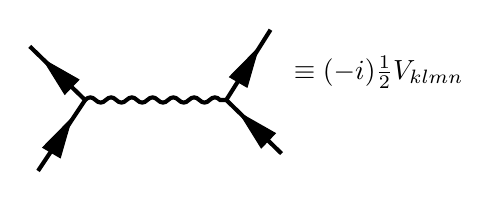
\begin{tikzpicture}[x=0.75pt,y=0.75pt,yscale=-1,xscale=1]
%uncomment if require: \path (0,705); %set diagram left start at 0, and has height of 705
%Straight Lines [id:da613823184290475] 
\draw [line width=1.5]    (436.42,562.13) .. controls (438.09,560.46) and (439.75,560.46) .. (441.42,562.13) .. controls (443.09,563.8) and (444.75,563.8) .. (446.42,562.13) .. controls (448.09,560.46) and (449.75,560.46) .. (451.42,562.13) .. controls (453.09,563.8) and (454.75,563.8) .. (456.42,562.13) .. controls (458.09,560.46) and (459.75,560.46) .. (461.42,562.13) .. controls (463.09,563.8) and (464.75,563.8) .. (466.42,562.13) .. controls (468.09,560.46) and (469.75,560.46) .. (471.42,562.13) .. controls (473.09,563.8) and (474.75,563.8) .. (476.42,562.13) .. controls (478.09,560.46) and (479.75,560.46) .. (481.42,562.13) .. controls (483.09,563.8) and (484.75,563.8) .. (486.42,562.13) .. controls (488.09,560.46) and (489.75,560.46) .. (491.42,562.13) .. controls (493.09,563.8) and (494.75,563.8) .. (496.42,562.13) .. controls (498.09,560.46) and (499.75,560.46) .. (501.42,562.13) -- (504.42,562.13) -- (504.42,562.13) ;
%Straight Lines [id:da6353755682299548] 
\draw [line width=1.5]    (409.75,536.3) -- (436.42,562.13) ;
%Straight Lines [id:da6254606220772768] 
\draw [line width=1.5]    (504.42,562.13) -- (531.08,587.97) ;
%Straight Lines [id:da5480869883300985] 
\draw [line width=1.5]    (436.42,562.13) -- (413.75,596.3) ;
%Straight Lines [id:da49445752084181116] 
\draw [line width=1.5]    (525.75,528.3) -- (504.42,562.13) ;
%Shape: Triangle [id:dp022384072825595847] 
\draw  [fill={rgb, 255:red, 0; green, 0; blue, 0 }  ,fill opacity=1 ] (416.18,542.57) -- (433.37,552.35) -- (426.61,559.37) -- cycle ;
%Shape: Triangle [id:dp5669679661948073] 
\draw  [fill={rgb, 255:red, 0; green, 0; blue, 0 }  ,fill opacity=1 ] (510.84,568.41) -- (528.04,578.18) -- (521.28,585.21) -- cycle ;
%Shape: Triangle [id:dp23872151900315752] 
\draw  [fill={rgb, 255:red, 0; green, 0; blue, 0 }  ,fill opacity=1 ] (519.92,536.94) -- (514.46,555.95) -- (506.04,551.03) -- cycle ;
%Shape: Triangle [id:dp5504301680867448] 
\draw  [fill={rgb, 255:red, 0; green, 0; blue, 0 }  ,fill opacity=1 ] (429.92,570.94) -- (424.46,589.95) -- (416.04,585.03) -- cycle ;

% Text Node
\draw (535.68,539.7) node [anchor=north west][inner sep=0.75pt]    {$\equiv ( -i)\frac{1}{2} V_{klmn}$};
\end{tikzpicture}
\end{center}
Using the particle-hole formalism, this may be drawn in more detail, thus:
\begin{equation}
    \includegraphics[width=0.8\textwidth]{screenshots/wiggly-diagram-types.PNG}
    \label{wiggly-types}
\end{equation}
Diagram (a) pictures scattering of two particles at state $\phi_m$ and $\phi_n$ into $\phi_k$ and $\phi_l$. In (b) a particle at state $\phi_m$ interacts with another particle below the Fermi surface in state $\phi_n$ to create a hole in $\phi_n$ and a particle in $\phi_l$. At the same time the original particle undergoes a transition to state $\phi_k$. Note that the diagrams in \ref{wiggly-types} correspond precisely to the interaction terms in the Hamiltonian of \ref{mutual-interact-hamiltonian}.
\begin{imp}
It is extremely important to note the labelling convention used in $V_{k l m n}: \mathbf{k}=$ line out of left vertex, $\mathbf{l}=$ line out of right vertex, $\mathbf{m}=$ line into left vertex, $\mathbf{n}=$ line into right vertex. A mnemonic aid is to remember the tango dance step: \textbf{left out, right out, left in, right in.}
\end{imp}
\redp{The interaction $V(|\mathbf{r}-\mathbf{r}^{\prime}|)$ only depends on the distance between the particles so it conserves linear and spin momentum.} Thus
$$\mathbf{k}+\mathbf{l}=\mathbf{m}+\mathbf{n} ; \quad \boldsymbol{\sigma}_{k}+\boldsymbol{\sigma}_{l}=\boldsymbol{\sigma}_{m}+\boldsymbol{\sigma}_{n}$$
We can incorporate this conservation law into our diagrams by labelling the "momentum flow" shown below:
\begin{equation}
\tikzset{every picture/.style={line width=0.75pt}} %set default line width to 0.75pt        
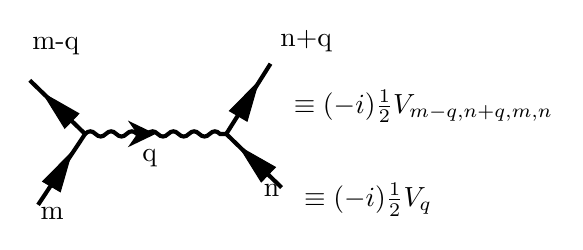
\begin{tikzpicture}[x=0.75pt,y=0.75pt,yscale=-1,xscale=1]
%uncomment if require: \path (0,705); %set diagram left start at 0, and has height of 705
%Straight Lines [id:da613823184290475] 
\draw [line width=1.5]    (416.42,563.13) .. controls (418.09,561.46) and (419.75,561.46) .. (421.42,563.13) .. controls (423.09,564.8) and (424.75,564.8) .. (426.42,563.13) .. controls (428.09,561.46) and (429.75,561.46) .. (431.42,563.13) .. controls (433.09,564.8) and (434.75,564.8) .. (436.42,563.13) .. controls (438.09,561.46) and (439.75,561.46) .. (441.42,563.13) .. controls (443.09,564.8) and (444.75,564.8) .. (446.42,563.13) .. controls (448.09,561.46) and (449.75,561.46) .. (451.42,563.13) .. controls (453.09,564.8) and (454.75,564.8) .. (456.42,563.13) .. controls (458.09,561.46) and (459.75,561.46) .. (461.42,563.13) .. controls (463.09,564.8) and (464.75,564.8) .. (466.42,563.13) .. controls (468.09,561.46) and (469.75,561.46) .. (471.42,563.13) .. controls (473.09,564.8) and (474.75,564.8) .. (476.42,563.13) .. controls (478.09,561.46) and (479.75,561.46) .. (481.42,563.13) -- (484.42,563.13) -- (484.42,563.13) ;
\draw [shift={(450.42,563.13)}, rotate = 180] [fill={rgb, 255:red, 0; green, 0; blue, 0 }  ][line width=0.08]  [draw opacity=0] (13.4,-6.43) -- (0,0) -- (13.4,6.44) -- (8.9,0) -- cycle    ;
%Straight Lines [id:da6353755682299548] 
\draw [line width=1.5]    (389.75,537.3) -- (416.42,563.13) ;
%Straight Lines [id:da6254606220772768] 
\draw [line width=1.5]    (484.42,563.13) -- (511.08,588.97) ;
%Straight Lines [id:da5480869883300985] 
\draw [line width=1.5]    (416.42,563.13) -- (393.75,597.3) ;
%Straight Lines [id:da49445752084181116] 
\draw [line width=1.5]    (505.75,529.3) -- (484.42,563.13) ;
%Shape: Triangle [id:dp022384072825595847] 
\draw  [fill={rgb, 255:red, 0; green, 0; blue, 0 }  ,fill opacity=1 ] (396.18,543.57) -- (413.37,553.35) -- (406.61,560.37) -- cycle ;
%Shape: Triangle [id:dp5669679661948073] 
\draw  [fill={rgb, 255:red, 0; green, 0; blue, 0 }  ,fill opacity=1 ] (490.84,569.41) -- (508.04,579.18) -- (501.28,586.21) -- cycle ;
%Shape: Triangle [id:dp23872151900315752] 
\draw  [fill={rgb, 255:red, 0; green, 0; blue, 0 }  ,fill opacity=1 ] (499.92,537.94) -- (494.46,556.95) -- (486.04,552.03) -- cycle ;
%Shape: Triangle [id:dp5504301680867448] 
\draw  [fill={rgb, 255:red, 0; green, 0; blue, 0 }  ,fill opacity=1 ] (409.92,571.94) -- (404.46,590.95) -- (396.04,586.03) -- cycle ;

% Text Node
\draw (515.68,540.7) node [anchor=north west][inner sep=0.75pt]    {$\equiv ( -i)\frac{1}{2} V_{m-q,n+q,m,n}$};
% Text Node
\draw (393.75,597.3) node [anchor=north west][inner sep=0.75pt]   [align=left] {m};
% Text Node
\draw (389.75,515.3) node [anchor=north west][inner sep=0.75pt]   [align=left] {m-q};
% Text Node
\draw (442.75,569.3) node [anchor=north west][inner sep=0.75pt]   [align=left] {q};
% Text Node
\draw (501.28,586.21) node [anchor=north west][inner sep=0.75pt]   [align=left] {n};
% Text Node
\draw (509.28,512.21) node [anchor=north west][inner sep=0.75pt]   [align=left] {n+q};
% Text Node
\draw (520.68,585.7) node [anchor=north west][inner sep=0.75pt]    {$\equiv ( -i)\frac{1}{2} V_{q}$};


\end{tikzpicture}
\label{momentum-flow}
\end{equation}
By changing the dummy indices in \ref{Vklmn-defi} we have $V_{klmn}=V_{lknm}$, so $V_q=V_{-q}$. $V_{-q}$ corresponds to the diagram in \ref{momentum-flow} twisted through $180^o$, has momentum transfer $\mathbf{q}^{\prime}=\mathbf{n}-\mathbf{l}$.
\begin{imp}
It is important to note that although the collisions conserves momentum, they do not conserve energy. For example, at the lower interaction of the diagram shown below we see the energy flow into the interaction \bluep{(in the unit of $\hbar^2/2m$)} is $k^2+l^2$, while the energy flow out is $(k-q)^2+(l+q)^2$. Hence we are dealing with virtual particles during the interactions.
\begin{center}
    


\tikzset{every picture/.style={line width=0.75pt}} %set default line width to 0.75pt        

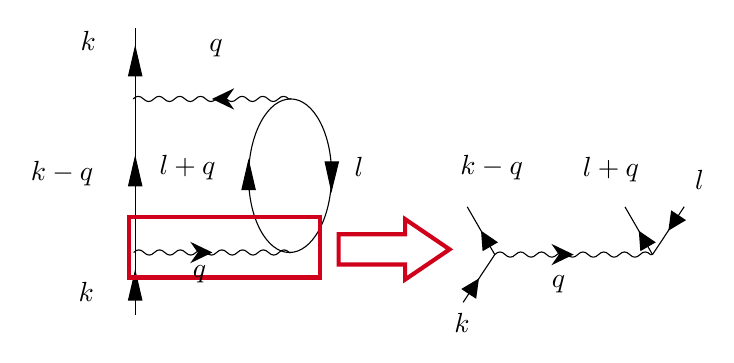
\begin{tikzpicture}[x=0.75pt,y=0.75pt,yscale=-1,xscale=1]
%uncomment if require: \path (0,244); %set diagram left start at 0, and has height of 244

%Straight Lines [id:da8265491360075683] 
\draw    (62.53,30.8) -- (62.53,168.8) ;
%Straight Lines [id:da7214893814207295] 
\draw    (61.53,64.8) .. controls (63.2,63.13) and (64.86,63.13) .. (66.53,64.8) .. controls (68.2,66.47) and (69.86,66.47) .. (71.53,64.8) .. controls (73.2,63.13) and (74.86,63.13) .. (76.53,64.8) .. controls (78.2,66.47) and (79.86,66.47) .. (81.53,64.8) .. controls (83.2,63.13) and (84.86,63.13) .. (86.53,64.8) .. controls (88.2,66.47) and (89.86,66.47) .. (91.53,64.8) .. controls (93.2,63.13) and (94.86,63.13) .. (96.53,64.8) .. controls (98.2,66.47) and (99.86,66.47) .. (101.53,64.8) .. controls (103.2,63.13) and (104.86,63.13) .. (106.53,64.8) .. controls (108.2,66.47) and (109.86,66.47) .. (111.53,64.8) .. controls (113.2,63.13) and (114.86,63.13) .. (116.53,64.8) .. controls (118.2,66.47) and (119.86,66.47) .. (121.53,64.8) .. controls (123.2,63.13) and (124.86,63.13) .. (126.53,64.8) .. controls (128.2,66.47) and (129.86,66.47) .. (131.53,64.8) .. controls (133.2,63.13) and (134.86,63.13) .. (136.53,64.8) -- (137.53,64.8) -- (137.53,64.8) ;
\draw [shift={(99.53,64.8)}, rotate = 0] [fill={rgb, 255:red, 0; green, 0; blue, 0 }  ][line width=0.08]  [draw opacity=0] (10.72,-5.15) -- (0,0) -- (10.72,5.15) -- (7.12,0) -- cycle    ;
%Straight Lines [id:da6531867980247327] 
\draw    (61.78,138.78) .. controls (63.45,137.11) and (65.11,137.11) .. (66.78,138.78) .. controls (68.45,140.45) and (70.11,140.45) .. (71.78,138.78) .. controls (73.45,137.11) and (75.11,137.11) .. (76.78,138.78) .. controls (78.45,140.45) and (80.11,140.45) .. (81.78,138.78) .. controls (83.45,137.11) and (85.11,137.11) .. (86.78,138.78) .. controls (88.45,140.45) and (90.11,140.45) .. (91.78,138.78) .. controls (93.45,137.11) and (95.11,137.11) .. (96.78,138.78) .. controls (98.45,140.45) and (100.11,140.45) .. (101.78,138.78) .. controls (103.45,137.11) and (105.11,137.11) .. (106.78,138.78) .. controls (108.45,140.45) and (110.11,140.45) .. (111.78,138.78) .. controls (113.45,137.11) and (115.11,137.11) .. (116.78,138.78) .. controls (118.45,140.45) and (120.11,140.45) .. (121.78,138.78) .. controls (123.45,137.11) and (125.11,137.11) .. (126.78,138.78) .. controls (128.45,140.45) and (130.11,140.45) .. (131.78,138.78) .. controls (133.45,137.11) and (135.11,137.11) .. (136.78,138.78) -- (137.78,138.78) -- (137.78,138.78) ;
\draw [shift={(99.78,138.78)}, rotate = 180] [fill={rgb, 255:red, 0; green, 0; blue, 0 }  ][line width=0.08]  [draw opacity=0] (10.72,-5.15) -- (0,0) -- (10.72,5.15) -- (7.12,0) -- cycle    ;
%Shape: Ellipse [id:dp27679763462197615] 
\draw   (136.78,138.78) .. controls (125.74,138.67) and (116.95,122.02) .. (117.16,101.59) .. controls (117.37,81.16) and (126.49,64.69) .. (137.53,64.8) .. controls (148.58,64.91) and (157.36,81.56) .. (157.16,101.99) .. controls (156.95,122.42) and (147.83,138.89) .. (136.78,138.78) -- cycle ;
%Shape: Triangle [id:dp5635326143074989] 
\draw  [fill={rgb, 255:red, 0; green, 0; blue, 0 }  ,fill opacity=1 ] (117.16,94.73) -- (120.35,108.45) -- (113.97,108.45) -- cycle ;
%Shape: Triangle [id:dp24603935178928227] 
\draw  [fill={rgb, 255:red, 0; green, 0; blue, 0 }  ,fill opacity=1 ] (157.07,108.86) -- (154.06,95.09) -- (160.44,95.17) -- cycle ;
%Shape: Triangle [id:dp6426129992054267] 
\draw  [fill={rgb, 255:red, 0; green, 0; blue, 0 }  ,fill opacity=1 ] (62.53,92.94) -- (65.72,106.66) -- (59.35,106.66) -- cycle ;
%Shape: Triangle [id:dp6567192777691618] 
\draw  [fill={rgb, 255:red, 0; green, 0; blue, 0 }  ,fill opacity=1 ] (62.53,39.94) -- (65.72,53.66) -- (59.35,53.66) -- cycle ;
%Shape: Triangle [id:dp3743764640683508] 
\draw  [fill={rgb, 255:red, 0; green, 0; blue, 0 }  ,fill opacity=1 ] (62.53,147.94) -- (65.72,161.66) -- (59.35,161.66) -- cycle ;
%Shape: Rectangle [id:dp8012947756470761] 
\draw  [color={rgb, 255:red, 208; green, 2; blue, 27 }  ,draw opacity=1 ][line width=1.5]  (59.35,121.66) -- (151.53,121.66) -- (151.53,150.8) -- (59.35,150.8) -- cycle ;
%Right Arrow [id:dp412985882083701] 
\draw  [color={rgb, 255:red, 208; green, 2; blue, 27 }  ,draw opacity=1 ][line width=1.5]  (160.53,130) -- (192.61,130) -- (192.61,122.73) -- (214,137.27) -- (192.61,151.8) -- (192.61,144.53) -- (160.53,144.53) -- cycle ;
%Straight Lines [id:da9760212638037913] 
\draw    (235.78,139.78) .. controls (237.45,138.11) and (239.11,138.11) .. (240.78,139.78) .. controls (242.45,141.45) and (244.11,141.45) .. (245.78,139.78) .. controls (247.45,138.11) and (249.11,138.11) .. (250.78,139.78) .. controls (252.45,141.45) and (254.11,141.45) .. (255.78,139.78) .. controls (257.45,138.11) and (259.11,138.11) .. (260.78,139.78) .. controls (262.45,141.45) and (264.11,141.45) .. (265.78,139.78) .. controls (267.45,138.11) and (269.11,138.11) .. (270.78,139.78) .. controls (272.45,141.45) and (274.11,141.45) .. (275.78,139.78) .. controls (277.45,138.11) and (279.11,138.11) .. (280.78,139.78) .. controls (282.45,141.45) and (284.11,141.45) .. (285.78,139.78) .. controls (287.45,138.11) and (289.11,138.11) .. (290.78,139.78) .. controls (292.45,141.45) and (294.11,141.45) .. (295.78,139.78) .. controls (297.45,138.11) and (299.11,138.11) .. (300.78,139.78) .. controls (302.45,141.45) and (304.11,141.45) .. (305.78,139.78) .. controls (307.45,138.11) and (309.11,138.11) .. (310.78,139.78) -- (311.78,139.78) -- (311.78,139.78) ;
\draw [shift={(273.78,139.78)}, rotate = 180] [fill={rgb, 255:red, 0; green, 0; blue, 0 }  ][line width=0.08]  [draw opacity=0] (10.72,-5.15) -- (0,0) -- (10.72,5.15) -- (7.12,0) -- cycle    ;
%Straight Lines [id:da4571267837545099] 
\draw    (222.53,116.8) -- (235.78,139.78) ;
\draw [shift={(229.16,128.29)}, rotate = 60.03] [fill={rgb, 255:red, 0; green, 0; blue, 0 }  ][line width=0.08]  [draw opacity=0] (8.93,-4.29) -- (0,0) -- (8.93,4.29) -- cycle    ;
%Straight Lines [id:da08135471840003439] 
\draw    (235.78,139.78) -- (220.53,162.8) ;
\draw [shift={(228.16,151.29)}, rotate = 123.53] [fill={rgb, 255:red, 0; green, 0; blue, 0 }  ][line width=0.08]  [draw opacity=0] (8.93,-4.29) -- (0,0) -- (8.93,4.29) -- cycle    ;
%Straight Lines [id:da42744127070386173] 
\draw    (327.04,116.76) -- (311.78,139.78) ;
\draw [shift={(319.41,128.27)}, rotate = 303.53] [fill={rgb, 255:red, 0; green, 0; blue, 0 }  ][line width=0.08]  [draw opacity=0] (8.93,-4.29) -- (0,0) -- (8.93,4.29) -- cycle    ;
%Straight Lines [id:da3731869684683673] 
\draw    (298.53,116.8) -- (311.78,139.78) ;
\draw [shift={(305.16,128.29)}, rotate = 60.03] [fill={rgb, 255:red, 0; green, 0; blue, 0 }  ][line width=0.08]  [draw opacity=0] (8.93,-4.29) -- (0,0) -- (8.93,4.29) -- cycle    ;

% Text Node
\draw (11,93.73) node [anchor=north west][inner sep=0.75pt]    {$k-q$};
% Text Node
\draw (35,30.73) node [anchor=north west][inner sep=0.75pt]    {$k$};
% Text Node
\draw (34,151.73) node [anchor=north west][inner sep=0.75pt]    {$k$};
% Text Node
\draw (73,90.73) node [anchor=north west][inner sep=0.75pt]    {$l+q$};
% Text Node
\draw (167,91.73) node [anchor=north west][inner sep=0.75pt]    {$l$};
% Text Node
\draw (97,34.73) node [anchor=north west][inner sep=0.75pt]    {$q$};
% Text Node
\draw (89,143.73) node [anchor=north west][inner sep=0.75pt]    {$q$};
% Text Node
\draw (218,90.73) node [anchor=north west][inner sep=0.75pt]    {$k-q$};
% Text Node
\draw (215,166.73) node [anchor=north west][inner sep=0.75pt]    {$k$};
% Text Node
\draw (262,148.73) node [anchor=north west][inner sep=0.75pt]    {$q$};
% Text Node
\draw (331,97.73) node [anchor=north west][inner sep=0.75pt]    {$l$};
% Text Node
\draw (277,91.73) node [anchor=north west][inner sep=0.75pt]    {$l+q$};


\end{tikzpicture}
\end{center}
\end{imp}
The diagram in the box above depicts a particle in $\mathbf{k}$ being scattered into $\mathbf{k}-\mathbf{q}$ and simultaneously knocking a particle out of $\mathbf{l}$ into $\mathbf{l}+\mathbf{q}$ (i.e., creating a particle in $\mathbf{l}+\mathbf{q}$ and a hole in $\mathbf{l}$. At later time, the particle in $\mathbf{k}-\mathbf{q}$ knocks the particle in $\mathbf{l}+\mathbf{q}$ back into the hole state $\mathbf{l}$ (thus annihilating the particle-hole pair) and is itself scattered into state $\mathbf{k}$. \textbf{This is a second-order process, because it involves two interactions.}

The possibilities of first-order interactions are shown below
\begin{equation}
    \includegraphics[width=0.8\textwidth]{screenshots/first-order-wiggly.PNG}
\end{equation}
The diagrams such as
\begin{center}
\tikzset{every picture/.style={line width=0.75pt}} %set default line width to 0.75pt        

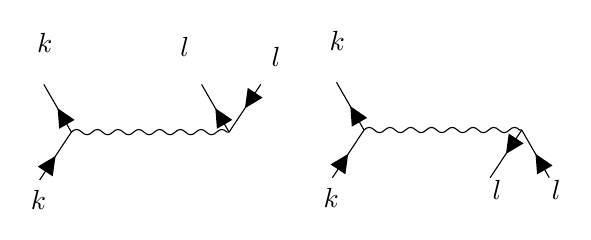
\begin{tikzpicture}[x=0.75pt,y=0.75pt,yscale=-1,xscale=1]
%uncomment if require: \path (0,244); %set diagram left start at 0, and has height of 244

%Straight Lines [id:da9760212638037913] 
\draw    (93.78,111.78) .. controls (95.45,110.11) and (97.11,110.11) .. (98.78,111.78) .. controls (100.45,113.45) and (102.11,113.45) .. (103.78,111.78) .. controls (105.45,110.11) and (107.11,110.11) .. (108.78,111.78) .. controls (110.45,113.45) and (112.11,113.45) .. (113.78,111.78) .. controls (115.45,110.11) and (117.11,110.11) .. (118.78,111.78) .. controls (120.45,113.45) and (122.11,113.45) .. (123.78,111.78) .. controls (125.45,110.11) and (127.11,110.11) .. (128.78,111.78) .. controls (130.45,113.45) and (132.11,113.45) .. (133.78,111.78) .. controls (135.45,110.11) and (137.11,110.11) .. (138.78,111.78) .. controls (140.45,113.45) and (142.11,113.45) .. (143.78,111.78) .. controls (145.45,110.11) and (147.11,110.11) .. (148.78,111.78) .. controls (150.45,113.45) and (152.11,113.45) .. (153.78,111.78) .. controls (155.45,110.11) and (157.11,110.11) .. (158.78,111.78) .. controls (160.45,113.45) and (162.11,113.45) .. (163.78,111.78) .. controls (165.45,110.11) and (167.11,110.11) .. (168.78,111.78) -- (169.78,111.78) -- (169.78,111.78) ;
%Straight Lines [id:da4571267837545099] 
\draw    (80.53,88.8) -- (93.78,111.78) ;
\draw [shift={(87.16,100.29)}, rotate = 60.03] [fill={rgb, 255:red, 0; green, 0; blue, 0 }  ][line width=0.08]  [draw opacity=0] (8.93,-4.29) -- (0,0) -- (8.93,4.29) -- cycle    ;
%Straight Lines [id:da08135471840003439] 
\draw    (93.78,111.78) -- (78.53,134.8) ;
\draw [shift={(86.16,123.29)}, rotate = 123.53] [fill={rgb, 255:red, 0; green, 0; blue, 0 }  ][line width=0.08]  [draw opacity=0] (8.93,-4.29) -- (0,0) -- (8.93,4.29) -- cycle    ;
%Straight Lines [id:da42744127070386173] 
\draw    (185.04,88.76) -- (169.78,111.78) ;
\draw [shift={(177.41,100.27)}, rotate = 303.53] [fill={rgb, 255:red, 0; green, 0; blue, 0 }  ][line width=0.08]  [draw opacity=0] (8.93,-4.29) -- (0,0) -- (8.93,4.29) -- cycle    ;
%Straight Lines [id:da3731869684683673] 
\draw    (156.53,88.8) -- (169.78,111.78) ;
\draw [shift={(163.16,100.29)}, rotate = 60.03] [fill={rgb, 255:red, 0; green, 0; blue, 0 }  ][line width=0.08]  [draw opacity=0] (8.93,-4.29) -- (0,0) -- (8.93,4.29) -- cycle    ;
%Straight Lines [id:da9023180120241947] 
\draw    (234.78,110.78) .. controls (236.45,109.11) and (238.11,109.11) .. (239.78,110.78) .. controls (241.45,112.45) and (243.11,112.45) .. (244.78,110.78) .. controls (246.45,109.11) and (248.11,109.11) .. (249.78,110.78) .. controls (251.45,112.45) and (253.11,112.45) .. (254.78,110.78) .. controls (256.45,109.11) and (258.11,109.11) .. (259.78,110.78) .. controls (261.45,112.45) and (263.11,112.45) .. (264.78,110.78) .. controls (266.45,109.11) and (268.11,109.11) .. (269.78,110.78) .. controls (271.45,112.45) and (273.11,112.45) .. (274.78,110.78) .. controls (276.45,109.11) and (278.11,109.11) .. (279.78,110.78) .. controls (281.45,112.45) and (283.11,112.45) .. (284.78,110.78) .. controls (286.45,109.11) and (288.11,109.11) .. (289.78,110.78) .. controls (291.45,112.45) and (293.11,112.45) .. (294.78,110.78) .. controls (296.45,109.11) and (298.11,109.11) .. (299.78,110.78) .. controls (301.45,112.45) and (303.11,112.45) .. (304.78,110.78) .. controls (306.45,109.11) and (308.11,109.11) .. (309.78,110.78) -- (310.78,110.78) -- (310.78,110.78) ;
%Straight Lines [id:da768308410681679] 
\draw    (221.53,87.8) -- (234.78,110.78) ;
\draw [shift={(228.16,99.29)}, rotate = 60.03] [fill={rgb, 255:red, 0; green, 0; blue, 0 }  ][line width=0.08]  [draw opacity=0] (8.93,-4.29) -- (0,0) -- (8.93,4.29) -- cycle    ;
%Straight Lines [id:da7130025901944149] 
\draw    (234.78,110.78) -- (219.53,133.8) ;
\draw [shift={(227.16,122.29)}, rotate = 123.53] [fill={rgb, 255:red, 0; green, 0; blue, 0 }  ][line width=0.08]  [draw opacity=0] (8.93,-4.29) -- (0,0) -- (8.93,4.29) -- cycle    ;
%Straight Lines [id:da8657016622612258] 
\draw    (310.78,110.78) -- (295.53,133.8) ;
\draw [shift={(303.16,122.29)}, rotate = 303.53] [fill={rgb, 255:red, 0; green, 0; blue, 0 }  ][line width=0.08]  [draw opacity=0] (8.93,-4.29) -- (0,0) -- (8.93,4.29) -- cycle    ;
%Straight Lines [id:da9413606756365827] 
\draw    (310.78,110.78) -- (324.04,133.76) ;
\draw [shift={(317.41,122.27)}, rotate = 60.03] [fill={rgb, 255:red, 0; green, 0; blue, 0 }  ][line width=0.08]  [draw opacity=0] (8.93,-4.29) -- (0,0) -- (8.93,4.29) -- cycle    ;

% Text Node
\draw (76,62.73) node [anchor=north west][inner sep=0.75pt]    {$k$};
% Text Node
\draw (73,138.73) node [anchor=north west][inner sep=0.75pt]    {$k$};
% Text Node
\draw (189,69.73) node [anchor=north west][inner sep=0.75pt]    {$l$};
% Text Node
\draw (145,64.73) node [anchor=north west][inner sep=0.75pt]    {$l$};
% Text Node
\draw (217,61.73) node [anchor=north west][inner sep=0.75pt]    {$k$};
% Text Node
\draw (214,137.73) node [anchor=north west][inner sep=0.75pt]    {$k$};
% Text Node
\draw (324.04,133.76) node [anchor=north west][inner sep=0.75pt]    {$l$};
% Text Node
\draw (295.53,133.8) node [anchor=north west][inner sep=0.75pt]    {$l$};


\end{tikzpicture}
\end{center}
are \bluep{not allowed since they have a particle and a hole in the same state $\mathbf{l}$.} It can be shown that diagrams (1),(3),(5) and (7) above do not occur either. The term in disturbed Hamiltonian that corresponds to (1) is 
\begin{equation}
    V_{klkl}a^{\dagger}_ka^{\dagger}_la_ka_l
\end{equation}
when this acts on the state with one incoming particle in $\phi_k$, we find
$$V_{k l k l} a_{k}^{\dagger} a_{l}^{\dagger} a_{k} a_{l}|1^p_k\rangle=0$$
Diagrams (3),(5), and (7) are similarly eliminated. Note that the term in $H_1$ corresponding to diagram (2) is (following the rule of left-out,right-out, left-in,right-in):
\begin{equation}V_{k l k l} a_{k}^{\dagger}b_l a_{k} b_{l}^{\dagger}\end{equation}
and
\begin{equation}V_{k l k l}  a_{k}^{\dagger}b_{l} a_{k} b_{l}^{\dagger}\left|1_{k}^{p}\right\rangle=V_{k l k l}\left|1_{k}^{p}\right\rangle \neq 0\end{equation}
The possible first-order processes may then be drawn using (2),(4),(6),(8). \textbf{This can only be done in one way, e.g., by in each case attaching the outgoing $\mathbf{l}$ line to the incoming one. Thus we find:}
\begin{equation}
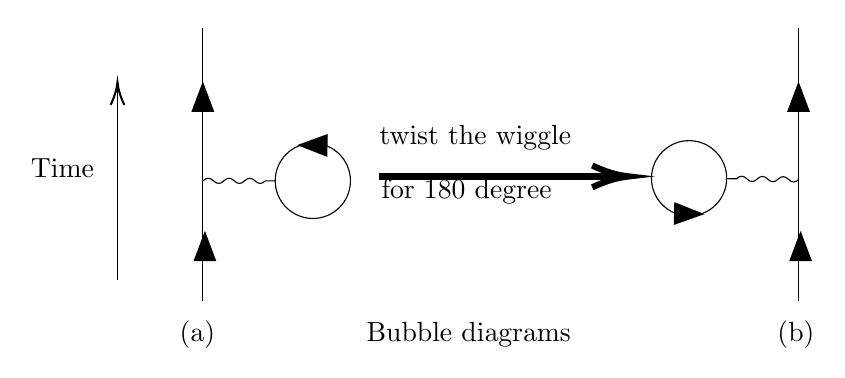
\begin{tikzpicture}[x=0.75pt,y=0.75pt,yscale=-1,xscale=1]
%uncomment if require: \path (0,235); %set diagram left start at 0, and has height of 235

%Straight Lines [id:da10068577398388545] 
\draw    (172,46.6) -- (172,178) ;
%Shape: Triangle [id:dp19925235312138345] 
\draw  [fill={rgb, 255:red, 0; green, 0; blue, 0 }  ,fill opacity=1 ] (172.13,73) -- (177.25,86.6) -- (167,86.6) -- cycle ;
%Shape: Triangle [id:dp004394430560968221] 
\draw  [fill={rgb, 255:red, 0; green, 0; blue, 0 }  ,fill opacity=1 ] (173.13,145) -- (178.25,158.6) -- (168,158.6) -- cycle ;
%Shape: Circle [id:dp41514745661808317] 
\draw   (207,120.13) .. controls (207,110.11) and (215.11,102) .. (225.13,102) .. controls (235.14,102) and (243.25,110.11) .. (243.25,120.13) .. controls (243.25,130.14) and (235.14,138.25) .. (225.13,138.25) .. controls (215.11,138.25) and (207,130.14) .. (207,120.13) -- cycle ;
%Straight Lines [id:da9922958867186198] 
\draw    (172.25,120.13) .. controls (173.92,118.46) and (175.58,118.46) .. (177.25,120.13) .. controls (178.92,121.8) and (180.58,121.8) .. (182.25,120.13) .. controls (183.92,118.46) and (185.58,118.46) .. (187.25,120.13) .. controls (188.92,121.8) and (190.58,121.8) .. (192.25,120.13) .. controls (193.92,118.46) and (195.58,118.46) .. (197.25,120.13) .. controls (198.92,121.8) and (200.58,121.8) .. (202.25,120.13) -- (207,120.13) -- (207,120.13) ;
%Shape: Triangle [id:dp2263151698703949] 
\draw  [fill={rgb, 255:red, 0; green, 0; blue, 0 }  ,fill opacity=1 ] (218.33,102.93) -- (231.98,97.95) -- (231.87,108.19) -- cycle ;
%Straight Lines [id:da3409503459639508] 
\draw    (459,46.6) -- (459,178) ;
%Shape: Triangle [id:dp7202483298889484] 
\draw  [fill={rgb, 255:red, 0; green, 0; blue, 0 }  ,fill opacity=1 ] (459.13,73) -- (464.25,86.6) -- (454,86.6) -- cycle ;
%Shape: Triangle [id:dp05921608545174617] 
\draw  [fill={rgb, 255:red, 0; green, 0; blue, 0 }  ,fill opacity=1 ] (460.13,145) -- (465.25,158.6) -- (455,158.6) -- cycle ;
%Shape: Circle [id:dp43994714997441664] 
\draw   (424.52,119.08) .. controls (424.42,129.09) and (416.22,137.12) .. (406.21,137.01) .. controls (396.2,136.91) and (388.17,128.71) .. (388.27,118.7) .. controls (388.38,108.69) and (396.58,100.66) .. (406.59,100.76) .. controls (416.6,100.87) and (424.63,109.07) .. (424.52,119.08) -- cycle ;
%Straight Lines [id:da8513266846637301] 
\draw    (459.27,119.44) .. controls (457.58,121.09) and (455.92,121.08) .. (454.27,119.39) .. controls (452.62,117.71) and (450.95,117.69) .. (449.27,119.34) .. controls (447.59,120.99) and (445.92,120.97) .. (444.27,119.29) .. controls (442.62,117.6) and (440.96,117.58) .. (439.27,119.23) .. controls (437.59,120.88) and (435.92,120.86) .. (434.27,119.18) .. controls (432.62,117.5) and (430.95,117.48) .. (429.27,119.13) -- (424.52,119.08) -- (424.52,119.08) ;
%Shape: Triangle [id:dp20595976463490984] 
\draw  [fill={rgb, 255:red, 0; green, 0; blue, 0 }  ,fill opacity=1 ] (413.02,136.15) -- (399.31,141) -- (399.53,130.75) -- cycle ;
%Straight Lines [id:da9038937323503633] 
\draw [line width=2.25]    (257,118) -- (373.25,118) ;
\draw [shift={(377.25,118)}, rotate = 180] [color={rgb, 255:red, 0; green, 0; blue, 0 }  ][line width=2.25]    (17.49,-5.26) .. controls (11.12,-2.23) and (5.29,-0.48) .. (0,0) .. controls (5.29,0.48) and (11.12,2.23) .. (17.49,5.26)   ;
%Straight Lines [id:da5407884786763255] 
\draw    (131,168) -- (131,74.6) ;
\draw [shift={(131,72.6)}, rotate = 450] [color={rgb, 255:red, 0; green, 0; blue, 0 }  ][line width=0.75]    (10.93,-3.29) .. controls (6.95,-1.4) and (3.31,-0.3) .. (0,0) .. controls (3.31,0.3) and (6.95,1.4) .. (10.93,3.29)   ;

% Text Node
\draw (256,92) node [anchor=north west][inner sep=0.75pt]   [align=left] {twist the wiggle};
% Text Node
\draw (257,118) node [anchor=north west][inner sep=0.75pt]   [align=left] {for 180 degree};
% Text Node
\draw (88,108) node [anchor=north west][inner sep=0.75pt]   [align=left] {Time};
% Text Node
\draw (159.73,186.07) node [anchor=north west][inner sep=0.75pt]   [align=left] {(a)};
% Text Node
\draw (447.73,186.07) node [anchor=north west][inner sep=0.75pt]   [align=left] {(b)};
% Text Node
\draw (249.73,187.07) node [anchor=north west][inner sep=0.75pt]   [align=left] {Bubble diagrams};


\end{tikzpicture}
\label{bubble-diagrams}
\end{equation}
\begin{equation}
    \includegraphics[width=0.8\textwidth]{screenshots/open-oyster-diagrams.PNG}
    \label{open-oyster-diagrams}
\end{equation}
The bubble processes can be physically interpreted as follows: a particle enters in $\mathbf{k}>k_F$, knocks a particle out of state $\mathbf{l}<k_F$ at time t, then knocks the particle instantaneously back into $\mathbf{l}$ at time t, then continues freely in state $\mathbf{k}$.

The open-oyster processes are just like the bubbles, except that a quick change act occurs in which at time $t$ the incoming particle simultaneously
(a) strikes the particle in $\mathbf{l},(b)$ creates an instantaneous hole in $\mathbf{l}$ and $(c)$ is exchanged for the particle in $\mathbf{l}.$ Diagrams \ref{open-oyster-diagrams}) are often called "first-order exchange diagrams', and the process is referred to as an \textbf{"exchange scattering"}. The instantaneous hole lines in the bubble and open oyster are called \textbf{"non-propagating"} lines.

We now see how to evaluate these diagrams. Consider \ref{bubble-diagrams}(a), we have
\begin{equation}\begin{array}{l}
G^+(\mathbf{k},t_2-t_1)=(-1) \sum_{l<k_{F}} \int_{-\infty}^{+\infty} d t\left[i G_{0}^{+}\left(\mathbf{k}, t-t_{1}\right)\right] \times\left[-\frac{i}{2} V_{k l k l}\right] \times \\
\quad \times\left[i G_{0}^{-}(l, t-t)\right] \times\left[i G_{0}^{+}\left(\mathbf{k}, t_{2}-t\right)\right]
\end{array}\end{equation}
\redp{The extra factor of (-1) in front comes from the fact that the diagram contains one \textbf{"fermion loop"}.} Note that an additional factor of (-1) appears because the propagator line for the bubble is:
\begin{equation}i G_{0}^{-}(1, t-t)=i \times i e^{-i\epsilon_l \times 0}=-1\end{equation}
The Fourier transform is then
\begin{equation}
G^+(\mathbf{k},\omega)=(-1)\left[i G_{0}^{+}(\mathbf{k}, \omega)\right]^{2} \sum_{i<k_{r}}\left[-\frac{i}{2} V_{k l k l}\right](-1)\end{equation}
In a similar fashion, \ref{bubble-diagrams}(b) is
\begin{equation}(-1)\left[i G^+(\mathbf{k},\omega)=G_{0}(\mathbf{k}, \omega)\right]^{2} \sum_{l<k_{r}}\left(-\frac{i}{2}\right) V_{l k l k}(-1)\end{equation}
Since $V_{klkl}=V_{lklk}$ these diagrams are equivalent. From here, we have the following rule:
\begin{imp}
If we are given a diagram, and form a new diagram from it by twisting one or more of its interaction wiggles through 180 degrees, then the new diagram has the same value as the original one. Hence all twisted diagrams may be omitted if we just multiply a correct factor in front.
\end{imp}
In a manner similar to the bubble diagram calculation, the open oyser gives
\begin{equation}
    G^+(\mathbf{k},\omega)=[iG^+_0(\mathbf{k},\omega)]^2\sum_{l<k_F}(-i)V_{lkkl}(-1)
\end{equation}
where the factor of 2 is included, and (-1) comes from $G^{-}_0(\mathbf{k},t-t)$. Observe that the frequency, $\omega$, associated with the propagator line coming out of the interaction is the same as that entering. This is an illustration of "\textbf{conservation of frequency}", and it is a result from the fact that \redp{the Hamiltonian is time-dependent.}

We now summarize the dictionary for the expansion series
\begin{figure}
    \centering
    \includegraphics[width=0.8\textwidth]{screenshots/interacting-fermi-sys-dict.PNG}
    \caption{Diagram dictionary for interacting many-fermion system with no external potential (Goldstone method)}
    \label{fig:goldstone-interacting-fermi-dict}
\end{figure}
The diagrams may also be interpreted physically from a particular time $t_0$:
\begin{center}
    \includegraphics[width=0.8\textwidth]{screenshots/goldstone-particular-time.PNG}
\end{center}
At $t_{0}$ we see that besides the bare particle, there may exist in the many-body system two "virtual' particles plus one hole created by second-order process $d$ or two particles and a hole created by second-order sequence $e,$ and so on, with the particle plus three particle-hole pairs created during the eighth-order poodle process illustrating a typical higher-order case. That is, \textbf{the diagrams show all the particles and holes which may be kicked up by the bare particle as it churns through the Fermi sea.}
\subsection{The "quasi-physical" nature of Feynman diagrams}   
\newpage
\section{Ground State Energy and Vacuum Amplitude}
\subsection{Meaning of the vacuum amplitude}
One of the first many-body problems to be tackled by the field theoretical diagram techniques was that of finding the ground state energy $E_0$ of a system of interacting fermions. The diagrammatic methods in this chapter provide a neat way of handling nuclear and electron interactions. In both cases, we can perform a partial sum over an infinite series of infinite terms and get a finite result. In order to do this, it is necessary to have a general way of writing down the nth-order term in the ordinary perturbation series for $E_0$,i.e., in
\begin{equation}E_{0}=W_{0}+\left\langle\Phi_{0}\left|H_{1}\right| \Phi_{0}\right\rangle+\sum_{m \neq 0} \frac{\left\langle\Phi_{0}\left|H_{1}\right| \phi_{m}\right\rangle\left\langle\Phi_{m}\left|H_{1}\right| \Phi_{0}\right\rangle}{W_{0}-W_{m}}+\cdots
\label{time-indep-ground}
\end{equation}
\textbf{where $W_{0}, W_{m}$ are the ground and excited state energies of the unperturbed Hamiltonian, and $\Phi_{0}, \Phi_{m}$ are the corresponding wave functions. The general term is hard to obtain from the time-independent theory usually used to get (\ref{time-indep-ground}).} However, there is a time-dependent technique which gives a pictorial recipe for finding the desired nth-order term:\redp{\textbf{vacuum amplitude expansion.}}
\begin{imp}
The vacuum amplitude, $R(t),$ is defined as follows: Let $\Phi_{0}$ be the ground state of the unperturbed system (i.e., $\Phi_{0}$ is the \textbf{'Fermi vacuum'}). Then $R(t)$ is the probability amplitude that if the system is in $\Phi_{0}$ at time $0,$ and the external potential and/or interactions between particles are allowed to act, then the system will be in $\Phi_{0}$ at time $t .$ That is, $R(t)$ is the \textbf{\redp{'Fermi vacuum to Fermi vacuum transition amplitude'}}. $R(t)$ can also be called \textbf{"no-particle propagator"}.
\end{imp}
If there is no interaction, then the wave function at time $t$ will simply be $\Phi_0e^{-iW_0t}$ where $W_0$ is the ground state energy. If the interaction is now switched on at time $t=0$, the system will start to make transition from $\Phi_0$ to all possible N-particle states. Let the state after time $t$ be $\Psi(t)$, \bluep{\textbf{this must be obtainable fro m the ground state $\Phi_0$, by some sort of operation.}} Thus:
\begin{equation}\Psi(t)=U(t) \Phi_{0}\end{equation}
which may be regarded as the equation defining the \textbf{"time development operator"},$U(t)$. The probability amplitude $R(t)$ is thus:
\begin{imp}
\begin{equation}\begin{aligned}
R(t) &=\left(\Phi_{0} e^{-i W_{0} t}, \Psi(t)\right)=\int \Phi_{0}^{*} e^{+i W_{0} t} U(t) \Phi_{0} d \mathbf{r}_{1} \dots d \mathbf{r}_{N} \\
& \equiv\left\langle\Phi_{0}|U(t)| \Phi_{0}\right\rangle e^{+i W_{0} t}=\text { vacuum amplitude. }
\end{aligned}
\label{vac-amp-def}
\end{equation}
The importance of the vacuum amplitude lies in the fact that the ground state energy, $E_{0}$, may be obtained from it with the aid of the theorem
\begin{equation}E_{0}=W_{0}+\lim _{t \rightarrow \infty(1-i \eta)} i \frac{d}{d t} \ln R(t)
\label{ground-energy-theorem}
\end{equation}
where $\eta$ is an infinitesimal. Thus, if we can get a diagrammatic expansion of $R(t)$, then the diagram series for $E_0$ follows from \ref{ground-energy-theorem}.
\end{imp}
\begin{mybox}
The diagrammatic perturbation expansion of $R(t)$ is considerably more complicated because of the \textbf{"unlinked" diagrams (i.e. not all vertices are connected).} Lukily, the Logarithm of R turns out to be the sume over just \textbf{"linked diagrams"}. This is the famous \textbf{"linked cluster theorem"}.
\end{mybox}

\subsection{Quantum vacuum amplitude for one-particle system}
Consider the simplest situation first: a Fermi system consisting of one particle in an external potential, with non-degenerate energy levels-for example, an electron in a one-dimensional harmonic oscillator potential. Let the unperturbed Hamiltonian be
$$H_{0}=\frac{p^{2}}{2 m}+U(r)$$
with eigensolutions $\phi_k$,$\epsilon_k$. \bluep{The grpund state of the system consist of one particle in $\phi_1$ and no particles in any higher states;} in occupation number formalism this is $\Phi_0=|1_1,0_2,0_3,\ldots\rangle$. The corresponding ground state is just $W_0=\epsilon_1$. A typical excited state is one particle in $\phi_{k}$ and no particle in any other state: $\Phi_{\text {excited }}=\left|0_{1}, 0_{2}, \ldots, 1_{k}, \ldots\right\rangle .$ In particle-hole notation, the ground state is $\left.\Phi_{0}=|0\right\rangle,$ while a typical excited state consists of a hole in $\phi_{1}$ and a particle in $\phi_{k}: \Phi_{\text {exe }}=\left|1_{1}^{h}, 1_{k}^p\right\rangle .$ Note that in this one-particle system, there is only one possible hole state, e.g., $\phi_{1}$.

Suppose now a perturbation $V(\mathbf{r})$ is added to $H_{0} .$ The vacuum amplitude in that case is the probability amplitude that if the system starts in its ground state $\Phi_{0}$ at $t=0,$ and is acted upon zero or more times by $V(\mathrm{r}),$ then it will be in $\Phi_{0} e^{-iW_{0} t}$ at time $t .$ By analogy with the pinball case, $R(t)$ will be the sum of the probability amplitudes for all the different ways the system can start out in $\Phi_0$, interact with $V(\mathbf{r})$ arbitrary times and return to $\Phi_0$. \textbf{In the zeroth-order process, nothing at all happens as illustrated below:}
\begin{equation}
    \includegraphics[width=0.8\textwidth]{screenshots/single-electron-diagram-order.PNG}
    \label{single-electron-diagram-order}
\end{equation}
In second order, at $t_1$, $V(\mathbf{t})$ can scatter the particle up into the state $\phi_k$, thus simultaneously creating a hole in $\phi_1$ and a particle in $\phi_k$, and at $t_2$ scatter the particle back into $\phi_1$. The fourth-order ones are
\begin{equation}
    \includegraphics[width=0.8\textwidth]{screenshots/single-electron-4th-order.PNG}
    \label{single-electron-4th-order}
\end{equation}
Note that in the last two diagrams of (\ref{single-electron-4th-order}) there are two particle lines and two hole lines between $t_{2}$ and $t_{3},$ whereas our one-particle system can have at most one particle and one hole. However, it is easily shown that \textbf{these diagrams are exactly cancelled by unlinked diagrams of the sort in (\ref{single-electron-unlinked-diagram}) below}. 
\begin{equation}
    \includegraphics[width=0.8\textwidth]{screenshots/single-electron-unlinked-diagram.PNG}
    \label{single-electron-unlinked-diagram}
\end{equation}
For example, because of \textbf{the (-1) from the extra fermion loop}, the last diagram in (\ref{single-electron-4th-order}) is cancelled by the fourth-order diagram in (\ref{single-electron-unlinked-diagram}). \bluep{Nevertheless, it is necessary to retain such diagrams which violate conservation of particle number, in order to prove the linked cluster theorem.} The same argument holds for diagrams which violate the Pauli exclusion principle.

In order to draw all diagrams in $n$ th order, draw $n$ dots in a vertical row, label them $t_{1}, t_{2}, \ldots, t_{n}$ and connect them up in all possible \textbf{'topologically distinct'} (see below) ways with one line entering and one leaving each dot. For example in third order we find the six diagrams
\begin{center}
    \includegraphics[width=0.8\textwidth]{screenshots/single-electron-topo-distinct.PNG}
\end{center}
Two diagrams are ' \textbf{topologically equivalent}' if one can be \bluep{distorted into the other without changing the vertical ordering of the dots; otherwise they are distinct.} This is illustrated by the fourth-order diagrams (\textbf{note significance of the direction of the arrows}).

Finally, the diagrammatic expansion for the vacuum amplitude will just be the sum of all diagrams such as the above:
\begin{equation}
    \includegraphics[width=0.8\textwidth]{screenshots/single-electron-ground-expansion.PNG}
    \label{single-electron-ground-expansion}
\end{equation}
where the 1 expresses the fact that in the unperturbed case, the probability amplitude for the system staying in its ground state is 1. Translate the series into equation we have
\begin{equation}
    \begin{aligned}
    R(t)=1-&V_{11} \int_{0}^{t} d t_{1} G_{0}\left(1, t_{1}-t_{1}\right)-\\
    &-\sum_{p>1} V_{1p} V_{p 1} \int_{0}^{t} d t_{1} \int_{0}^{t} \underset{t_2>t_1}{dt_2} G_{0}^{+}\left(p, t_{2}-t_{1}\right) G_{0}^{-}\left(1, t_{1}-t_{2}\right)+\cdots\\
    &+V_{11} V_{11} \int_{0}^{t} d t_{1} \int_{0}^{t} \underset{t_2>t_1}{d t_{2}} \quad G_{0}^{-}\left(1, t_{1}-t_{1}\right) \sigma_{0}\left(1, t_{2}-t_{2}\right)+\cdots
    \end{aligned}
\end{equation}

\subsection{Linked cluster theorem for one-particle system}
The theorem states that
\begin{equation}
    lnR(t)=\Sigma\text{ all linked graphs}
    \label{single-electron-linked-theorem}
\end{equation}
The proof is based on the fact that \textbf{the contribution from a unlinked diagram is proportional to the product of the contribution of its various parts.} Consider for example the $V_{11}V_{11}$ term:
\begin{center}
\tikzset{every picture/.style={line width=0.75pt}} %set default line width to 0.75pt        
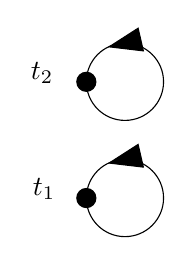
\begin{tikzpicture}[x=0.75pt,y=0.75pt,yscale=-1,xscale=1]
%uncomment if require: \path (0,244); %set diagram left start at 0, and has height of 244

%Shape: Circle [id:dp6498223397318404] 
\draw   (81,85.6) .. controls (81,75.33) and (89.33,67) .. (99.6,67) .. controls (109.87,67) and (118.2,75.33) .. (118.2,85.6) .. controls (118.2,95.87) and (109.87,104.2) .. (99.6,104.2) .. controls (89.33,104.2) and (81,95.87) .. (81,85.6) -- cycle ;
%Shape: Circle [id:dp27995222268876896] 
\draw  [fill={rgb, 255:red, 0; green, 0; blue, 0 }  ,fill opacity=1 ] (76.4,85.6) .. controls (76.4,83.06) and (78.46,81) .. (81,81) .. controls (83.54,81) and (85.6,83.06) .. (85.6,85.6) .. controls (85.6,88.14) and (83.54,90.2) .. (81,90.2) .. controls (78.46,90.2) and (76.4,88.14) .. (76.4,85.6) -- cycle ;
%Shape: Triangle [id:dp3898756772562222] 
\draw  [fill={rgb, 255:red, 0; green, 0; blue, 0 }  ,fill opacity=1 ] (92,68.75) -- (105.94,59.79) -- (108.46,70.7) -- cycle ;
%Shape: Circle [id:dp6531439047197907] 
\draw   (81,141.6) .. controls (81,131.33) and (89.33,123) .. (99.6,123) .. controls (109.87,123) and (118.2,131.33) .. (118.2,141.6) .. controls (118.2,151.87) and (109.87,160.2) .. (99.6,160.2) .. controls (89.33,160.2) and (81,151.87) .. (81,141.6) -- cycle ;
%Shape: Circle [id:dp7775379383850192] 
\draw  [fill={rgb, 255:red, 0; green, 0; blue, 0 }  ,fill opacity=1 ] (76.4,141.6) .. controls (76.4,139.06) and (78.46,137) .. (81,137) .. controls (83.54,137) and (85.6,139.06) .. (85.6,141.6) .. controls (85.6,144.14) and (83.54,146.2) .. (81,146.2) .. controls (78.46,146.2) and (76.4,144.14) .. (76.4,141.6) -- cycle ;
%Shape: Triangle [id:dp43271531457083345] 
\draw  [fill={rgb, 255:red, 0; green, 0; blue, 0 }  ,fill opacity=1 ] (92,124.75) -- (105.94,115.79) -- (108.46,126.7) -- cycle ;

% Text Node
\draw (54,131) node [anchor=north west][inner sep=0.75pt]    {$t_{1}$};
% Text Node
\draw (53,75) node [anchor=north west][inner sep=0.75pt]    {$t_{2}$};
\end{tikzpicture}
\end{center}
Translating it into equation we have
$$
\begin{aligned}
&V_{11} V_{11} \int_{0}^{t} d t_{1} \int_{0}^{t} \underset{t_2>t_1}{d t_{2}} G_{0}^{-} G_{0}^{-}=V_{11}^{2} G_{0}^{-2} \int_{0}^{t} d t_{1} \int_{0}^{t} \underset{t_2>t_1}{d t_{2}}\\
&=V_{11}^{2} G_{0}^{-2} \int_{0}^{t} d t_{1} \int_{0}^{t} d t_{2} \times \frac{1}{2} \quad \text { (where } t_{2}>\text { or }<t_{1})\\
&=\frac{1}{2}\left[V_{11} \int_{0}^{1} d t_{1} G_{0}^{-}\left(1, t_{1}-t_{1}\right)\right] \times\left[V_{11} \int_{0}^{t} d t_{2} G_{0}^{-}\left(1, t_{2}-t_{2}\right)\right]\\
&=\frac{1}{2!}\times\selfcirc^2
\end{aligned}
$$
In general, it turns out that the value of an unlinked diagram with $n$ identical links $L,$ is just $(1 / n !) \times L^{n}$.

A similar factorization occurs for non-identical links if we first sum over all possible time orders. For example, the following three graphs can be summed over:
\begin{center}
\tikzset{every picture/.style={line width=0.75pt}} %set default line width to 0.75pt        
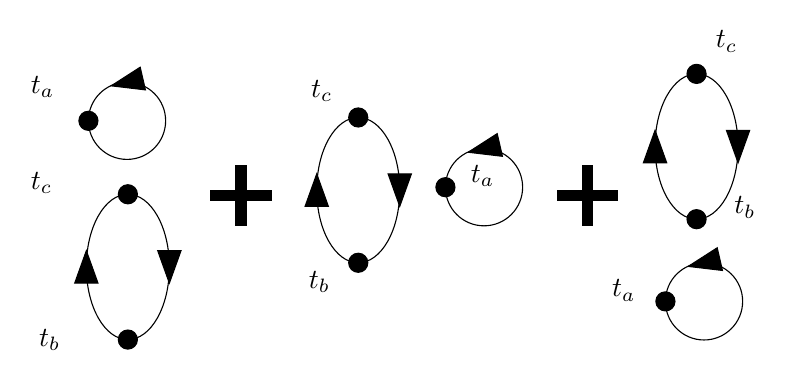
\begin{tikzpicture}[x=0.75pt,y=0.75pt,yscale=-1,xscale=1]
%uncomment if require: \path (0,244); %set diagram left start at 0, and has height of 244

%Shape: Circle [id:dp6498223397318404] 
\draw   (81,85.6) .. controls (81,75.33) and (89.33,67) .. (99.6,67) .. controls (109.87,67) and (118.2,75.33) .. (118.2,85.6) .. controls (118.2,95.87) and (109.87,104.2) .. (99.6,104.2) .. controls (89.33,104.2) and (81,95.87) .. (81,85.6) -- cycle ;
%Shape: Circle [id:dp27995222268876896] 
\draw  [fill={rgb, 255:red, 0; green, 0; blue, 0 }  ,fill opacity=1 ] (76.4,85.6) .. controls (76.4,83.06) and (78.46,81) .. (81,81) .. controls (83.54,81) and (85.6,83.06) .. (85.6,85.6) .. controls (85.6,88.14) and (83.54,90.2) .. (81,90.2) .. controls (78.46,90.2) and (76.4,88.14) .. (76.4,85.6) -- cycle ;
%Shape: Triangle [id:dp3898756772562222] 
\draw  [fill={rgb, 255:red, 0; green, 0; blue, 0 }  ,fill opacity=1 ] (92,68.75) -- (105.94,59.79) -- (108.46,70.7) -- cycle ;
%Shape: Ellipse [id:dp25610156841716825] 
\draw   (100,121) .. controls (111.05,121) and (120,136.67) .. (120,156) .. controls (120,175.33) and (111.05,191) .. (100,191) .. controls (88.95,191) and (80,175.33) .. (80,156) .. controls (80,136.67) and (88.95,121) .. (100,121) -- cycle ;
%Shape: Circle [id:dp9579907217839725] 
\draw  [fill={rgb, 255:red, 0; green, 0; blue, 0 }  ,fill opacity=1 ] (95.4,121) .. controls (95.4,118.46) and (97.46,116.4) .. (100,116.4) .. controls (102.54,116.4) and (104.6,118.46) .. (104.6,121) .. controls (104.6,123.54) and (102.54,125.6) .. (100,125.6) .. controls (97.46,125.6) and (95.4,123.54) .. (95.4,121) -- cycle ;
%Shape: Circle [id:dp44384941541376566] 
\draw  [fill={rgb, 255:red, 0; green, 0; blue, 0 }  ,fill opacity=1 ] (95.4,191) .. controls (95.4,188.46) and (97.46,186.4) .. (100,186.4) .. controls (102.54,186.4) and (104.6,188.46) .. (104.6,191) .. controls (104.6,193.54) and (102.54,195.6) .. (100,195.6) .. controls (97.46,195.6) and (95.4,193.54) .. (95.4,191) -- cycle ;
%Shape: Triangle [id:dp08449835110518966] 
\draw  [fill={rgb, 255:red, 0; green, 0; blue, 0 }  ,fill opacity=1 ] (120,163.8) -- (114.4,148.2) -- (125.6,148.2) -- cycle ;
%Shape: Triangle [id:dp33847857915014856] 
\draw  [fill={rgb, 255:red, 0; green, 0; blue, 0 }  ,fill opacity=1 ] (80,148.2) -- (85.6,163.8) -- (74.4,163.8) -- cycle ;
%Shape: Circle [id:dp16953709843220488] 
\draw   (253,117.6) .. controls (253,107.33) and (261.33,99) .. (271.6,99) .. controls (281.87,99) and (290.2,107.33) .. (290.2,117.6) .. controls (290.2,127.87) and (281.87,136.2) .. (271.6,136.2) .. controls (261.33,136.2) and (253,127.87) .. (253,117.6) -- cycle ;
%Shape: Circle [id:dp23125089891886985] 
\draw  [fill={rgb, 255:red, 0; green, 0; blue, 0 }  ,fill opacity=1 ] (248.4,117.6) .. controls (248.4,115.06) and (250.46,113) .. (253,113) .. controls (255.54,113) and (257.6,115.06) .. (257.6,117.6) .. controls (257.6,120.14) and (255.54,122.2) .. (253,122.2) .. controls (250.46,122.2) and (248.4,120.14) .. (248.4,117.6) -- cycle ;
%Shape: Triangle [id:dp3247983028310686] 
\draw  [fill={rgb, 255:red, 0; green, 0; blue, 0 }  ,fill opacity=1 ] (264,100.75) -- (277.94,91.79) -- (280.46,102.7) -- cycle ;
%Shape: Ellipse [id:dp473301006793975] 
\draw   (211,84) .. controls (222.05,84) and (231,99.67) .. (231,119) .. controls (231,138.33) and (222.05,154) .. (211,154) .. controls (199.95,154) and (191,138.33) .. (191,119) .. controls (191,99.67) and (199.95,84) .. (211,84) -- cycle ;
%Shape: Circle [id:dp7910773789667759] 
\draw  [fill={rgb, 255:red, 0; green, 0; blue, 0 }  ,fill opacity=1 ] (206.4,84) .. controls (206.4,81.46) and (208.46,79.4) .. (211,79.4) .. controls (213.54,79.4) and (215.6,81.46) .. (215.6,84) .. controls (215.6,86.54) and (213.54,88.6) .. (211,88.6) .. controls (208.46,88.6) and (206.4,86.54) .. (206.4,84) -- cycle ;
%Shape: Circle [id:dp29762035839742207] 
\draw  [fill={rgb, 255:red, 0; green, 0; blue, 0 }  ,fill opacity=1 ] (206.4,154) .. controls (206.4,151.46) and (208.46,149.4) .. (211,149.4) .. controls (213.54,149.4) and (215.6,151.46) .. (215.6,154) .. controls (215.6,156.54) and (213.54,158.6) .. (211,158.6) .. controls (208.46,158.6) and (206.4,156.54) .. (206.4,154) -- cycle ;
%Shape: Triangle [id:dp5382643640790852] 
\draw  [fill={rgb, 255:red, 0; green, 0; blue, 0 }  ,fill opacity=1 ] (231,126.8) -- (225.4,111.2) -- (236.6,111.2) -- cycle ;
%Shape: Triangle [id:dp787103954892548] 
\draw  [fill={rgb, 255:red, 0; green, 0; blue, 0 }  ,fill opacity=1 ] (191,111.2) -- (196.6,126.8) -- (185.4,126.8) -- cycle ;
%Shape: Circle [id:dp4980802915672331] 
\draw   (359,172.6) .. controls (359,162.33) and (367.33,154) .. (377.6,154) .. controls (387.87,154) and (396.2,162.33) .. (396.2,172.6) .. controls (396.2,182.87) and (387.87,191.2) .. (377.6,191.2) .. controls (367.33,191.2) and (359,182.87) .. (359,172.6) -- cycle ;
%Shape: Circle [id:dp9401870635500967] 
\draw  [fill={rgb, 255:red, 0; green, 0; blue, 0 }  ,fill opacity=1 ] (354.4,172.6) .. controls (354.4,170.06) and (356.46,168) .. (359,168) .. controls (361.54,168) and (363.6,170.06) .. (363.6,172.6) .. controls (363.6,175.14) and (361.54,177.2) .. (359,177.2) .. controls (356.46,177.2) and (354.4,175.14) .. (354.4,172.6) -- cycle ;
%Shape: Triangle [id:dp7535245748392855] 
\draw  [fill={rgb, 255:red, 0; green, 0; blue, 0 }  ,fill opacity=1 ] (370,155.75) -- (383.94,146.79) -- (386.46,157.7) -- cycle ;
%Shape: Ellipse [id:dp796880375497128] 
\draw   (374,63) .. controls (385.05,63) and (394,78.67) .. (394,98) .. controls (394,117.33) and (385.05,133) .. (374,133) .. controls (362.95,133) and (354,117.33) .. (354,98) .. controls (354,78.67) and (362.95,63) .. (374,63) -- cycle ;
%Shape: Circle [id:dp2607772888080764] 
\draw  [fill={rgb, 255:red, 0; green, 0; blue, 0 }  ,fill opacity=1 ] (369.4,63) .. controls (369.4,60.46) and (371.46,58.4) .. (374,58.4) .. controls (376.54,58.4) and (378.6,60.46) .. (378.6,63) .. controls (378.6,65.54) and (376.54,67.6) .. (374,67.6) .. controls (371.46,67.6) and (369.4,65.54) .. (369.4,63) -- cycle ;
%Shape: Circle [id:dp36338449977521137] 
\draw  [fill={rgb, 255:red, 0; green, 0; blue, 0 }  ,fill opacity=1 ] (369.4,133) .. controls (369.4,130.46) and (371.46,128.4) .. (374,128.4) .. controls (376.54,128.4) and (378.6,130.46) .. (378.6,133) .. controls (378.6,135.54) and (376.54,137.6) .. (374,137.6) .. controls (371.46,137.6) and (369.4,135.54) .. (369.4,133) -- cycle ;
%Shape: Triangle [id:dp6814504901438665] 
\draw  [fill={rgb, 255:red, 0; green, 0; blue, 0 }  ,fill opacity=1 ] (394,105.8) -- (388.4,90.2) -- (399.6,90.2) -- cycle ;
%Shape: Triangle [id:dp44737264879533356] 
\draw  [fill={rgb, 255:red, 0; green, 0; blue, 0 }  ,fill opacity=1 ] (354,90.2) -- (359.6,105.8) -- (348.4,105.8) -- cycle ;
%Shape: Cross [id:dp06220635309920053] 
\draw  [fill={rgb, 255:red, 0; green, 0; blue, 0 }  ,fill opacity=1 ] (152.1,107) -- (156.9,107) -- (156.9,119.1) -- (169,119.1) -- (169,123.9) -- (156.9,123.9) -- (156.9,136) -- (152.1,136) -- (152.1,123.9) -- (140,123.9) -- (140,119.1) -- (152.1,119.1) -- cycle ;
%Shape: Cross [id:dp6139216079282784] 
\draw  [fill={rgb, 255:red, 0; green, 0; blue, 0 }  ,fill opacity=1 ] (319.1,107) -- (323.9,107) -- (323.9,119.1) -- (336,119.1) -- (336,123.9) -- (323.9,123.9) -- (323.9,136) -- (319.1,136) -- (319.1,123.9) -- (307,123.9) -- (307,119.1) -- (319.1,119.1) -- cycle ;

% Text Node
\draw (52,109) node [anchor=north west][inner sep=0.75pt]    {$t_{c}$};
% Text Node
\draw (56,185) node [anchor=north west][inner sep=0.75pt]    {$t_{b}$};
% Text Node
\draw (52,63) node [anchor=north west][inner sep=0.75pt]    {$t_{a}$};
% Text Node
\draw (264,106) node [anchor=north west][inner sep=0.75pt]    {$t_{a}$};
% Text Node
\draw (187,65) node [anchor=north west][inner sep=0.75pt]    {$t_{c}$};
% Text Node
\draw (186,157) node [anchor=north west][inner sep=0.75pt]    {$t_{b}$};
% Text Node
\draw (391,121) node [anchor=north west][inner sep=0.75pt]    {$t_{b}$};
% Text Node
\draw (382,41) node [anchor=north west][inner sep=0.75pt]    {$t_{c}$};
% Text Node
\draw (332,161) node [anchor=north west][inner sep=0.75pt]    {$t_{a}$};


\end{tikzpicture}
\end{center}
Translate into equations we have
\begin{equation}\begin{array}{l}
\sum_{k} V_{k 1} V_{1 k} V_{11} \iiint d t_{a} d t_{b} d t_{c} \times \\
\quad \times G_{0}^{+}\left(k, t_{c}-t_{b}\right) G_{0}^{-}\left(1, t_{b}-t_{c}\right) G_{0}^{-}\left(1, t_{a}-t_{a}\right) x \\
\quad \times\left[\theta_{t_a-t_c}, \theta_{t_c-t_{b}}+\theta_{t_c-t_{a}} \theta_{t_{a}-t_{b}}+\theta_{t_c-t_b} \theta_{t_{b}-t_c}\right]\\
=\selfcirc\times\fermiloop
\end{array}\end{equation}
The $\theta^{\prime} s$ are used as a convenient way of writing the time order in the three diagrams. For $t_{c}>t_{b},$ some concentration shows that the term in brackets $=1$ regardless of where $t_{a}$ lies. This means the integral over $t_{a}$ is independent of that over $t_{b}$ and $t_{c},$ so the triple integral factorizes into two parts producing the result shown.

Combining these results, one finds that R may be written
\begin{equation}
\begin{aligned}
&\includegraphics[width=0.8\textwidth]{screenshots/single-electron-R.PNG}\\
&\includegraphics[width=0.8\textwidth]{screenshots/single-electron-R2.PNG}
\end{aligned}
\label{single-electron-R}
\end{equation}
In the many-body case, there is a deeper reason for the importance of the linked cluster theorem, e.g., \bluep{if we do not use it, we find that the perturbation series for the energy appears to diverge badly as the number of particles $N\rightarrow\infty$}.
\subsection{Finding the ground state energy in one-particle system}
Because the ground state energy depends only on the logarithm of $R$:
$$
E_{0}=\epsilon_{1}+\lim _{t \rightarrow \infty(1-i \eta)} i \frac{d}{d t} \ln R(t)
$$
it is now possible to obtain the expression for the ground state energy by translating the above diagrams into the following equations(remember \bluep{the (-1) factor in front of the "limit" is for the "fermion loop"}):
\begin{equation}
    \begin{aligned}
    E_{0}=&\epsilon_{1}-\lim _{n \rightarrow \infty(1-i\eta )} i \frac{d}{d t}\left\{(-i) V_{11} \int_{0}^{t} d t_{1} i G_{0}^{-}\left(1, t_{1}-t_{1}\right)+\right.\\
    &\left.+\sum_{p \neq 1}(-i)^{2} V_{1 p} V_{p 1} \int_{0}^{t} d t_{1} \int_{0}^{t} \underset{t_2>t_1}{d t_{2}} i G_{0}^{+}\left(p, t_{2}-t_{1}\right) i G_{0}^{-}\left(1, t_{1}-t_{2}\right)+\cdots\right\}
    \end{aligned}
\end{equation}
Thus, 
$$
E_0^{(1)}=\lim_{t\rightarrow\infty(1-i\eta)}i\frac{d}{dt}\selfcirc=V_{11}
$$
and the second term produces
$$
\begin{aligned}
\fermiloop&=(-1)^{2}(-i)^{2} \sum_{p \neq 1} V_{1 p} V_{p 1} \int_{0}^{1} d t_{1} \int_{0}^{t} d t_{2} \theta_{t_2-t_1} e^{-i\left(\epsilon_{p}-\epsilon_{1}\right)\left(t_{2}-t_{1}\right)}\\
&=(-1)^{2}(-i)^{2} \sum_{p \neq 1} V_{1 p} V_{p 1} \int_{0}^{t} d t_{1} \int_{0}^{t-t_{1}} d\left(t_{2}-t_{1}\right) e^{-i\left(\epsilon_{p}-\epsilon_1\right)\left(t_{2}-t_{1}\right)}
\end{aligned}
$$
Thus
$$
\lim _{t \rightarrow \infty(1-i\eta)} i \frac{d}{d t}\fermiloop=-i \sum_{p \neq 1} V_{1 p} V_{p 1}\left[-\frac{e^{-i\left(\epsilon_{p}-\epsilon_{1}\right) \omega(1-i \eta)}}{i\left(\epsilon_{p}-\epsilon_{1}\right)}+\frac{1}{i\left(\epsilon_{p}-\epsilon_{1}\right)}\right]
$$
or
\begin{equation}E_{0}^{(2)}=\sum_{p \neq 1} \frac{V_{1 p} V_{p 1}}{\epsilon_{1}-\epsilon_{p}}\end{equation}
where \redp{\textbf{the oscillating exponential is killed because $\left(\epsilon_{1}-\epsilon_{p}\right)$ and the infinitesimal $\eta \text { are both positive. (Note that } \eta \text { is chosen such that } \eta \times \infty=\infty .)$}} Proceeding in this way yields the third-and fourth-order terms:
\begin{equation}E_{0}^{(3)}=\sum_{p, q \neq 1} \frac{V_{1 p} V_{p q} V_{q 1}}{\left(\epsilon_{1}-\epsilon_{p}\right)\left(\epsilon_{1}-\epsilon_{q}\right)}-\sum_{p \neq 1} \frac{V_{1p}V_{p1} V_{11}}{\left(\epsilon_{1}-\epsilon_{p}\right)^{2}}
\label{single-electron-third-order}
\end{equation}
\begin{equation}
\begin{aligned}
E_{0}^{(4)}=& \sum_{p, q, r \neq 1} \frac{V_{1 p} V_{p q} V_{q r} V_{r 1}}{\left(\epsilon_{1}-\epsilon_{p}\right)\left(\epsilon_{1}-\epsilon_{q}\right)\left(\epsilon_{1}-\epsilon_{r}\right)}-\sum_{p, q \neq1} \frac{V_{1p} V_{p q} V_{q 1} V_{11}}{\left(\epsilon_{1}-\epsilon_{p}\right)^{2}\left(\epsilon_{1}-\epsilon_{q}\right)}-\\
&-\sum_{p, q \neq 1} \frac{V_{1 p} V_{p q} V_{q 1} V_{11}}{\left(\epsilon_{1}-\epsilon_{p}\right)\left(\epsilon_{1}-\epsilon_{q}\right)^{2}}+\sum_{p \neq 1} \frac{V_{1p} V_{p 1} V_{11} V_{11}}{\left(\epsilon_{1}-\epsilon_{p}\right)^{3}}-\\
&-\sum_{p, q \neq 1} \frac{V_{1 p} V_{p 1} V_{1 q} V_{q 1}}{\left(\epsilon_{1}-\epsilon_{p}\right)^{2}\left(\epsilon_{1}-\epsilon_{q}\right)}
\end{aligned}
\label{single-electron-fourth-order}
\end{equation}
This is the well-known Rayleigh-Schrodinger perturbation series carried out to fourth order. Now we use diagrammatic method to carry out the calculation to infinite order by \textbf{providing a systematic method for writing out the $nth-$order term in the expansion of $E_0$.}
\begin{imp}
To get the numerator of each term in (\ref{single-electron-third-order}-\ref{single-electron-fourth-order}), the product of $V_{kl}$ factors associated with the interaction dots will do. To get the denominator, draw light dotted horizontal lines \redp{between successive (in time) pairs of vertices}, thus
\begin{center}
    \includegraphics[width=0.8\textwidth]{screenshots/single-electron-denominator-rule.PNG}
\end{center}
and associated a factor of
\begin{equation}
    \frac{1}{\underset{\parbox{100pt}{\centering\tiny{all hole lines intersected by dotted line}}}{\Sigma \epsilon_1}-\underset{\parbox{100pt}{\centering\tiny{all particle lines intersected by dotted line}}}{\Sigma\epsilon_p}}
\end{equation}
The proper sign is obtained by multiplying by the factor $(-1)^{h+1}$ where h=number of hole lines in the diagram. The final rule is to sum over all particle indices.
\end{imp}
Applying these rules (which can be rigorously proved from the vacuum amplitude expansion) yields both of the third-order terms and they also produce the correct result in the other orders. (Note that in fourth order, the last term in (\ref{single-electron-fourth-order}) is obtained by summing the two "mitten" diagrams of (\ref{single-electron-4th-order}).)

Imagine that the perturbing potential is so large that it is impossible to get a decent result by using the usual method of cutting off the series after the first few orders. But suppose, for example, that the potential happens to have big matrix elements only between the ground and first excited states, i.e.,that $V_{12}$ and $V_{21}$ are large but all others are small. Then the perturbation series may be approximated by a partial sum over just those special diagrams in which all vertices connect '1' lines and '2' lines. This means that $E_0$ reduces to a sum over just the following diagrams
\begin{equation}
    \includegraphics[width=0.8\textwidth]{screenshots/single-electron-V12-series.PNG}
    \label{single-electron-V12-series}
\end{equation}
\bluep{Note that the odd-order diagrams do not occur. And each term representing a graph type is multiplied with a degeneracy factor}. Using the rules this series yields
\begin{equation}\begin{aligned}
E_{0} \approx \epsilon_{1} &+\frac{\left|V_{12}\right|^{2}}{\epsilon_{1}-\epsilon_{2}}-\frac{\left|V_{12}\right|^{4}}{\left(\epsilon_{1}-\epsilon_{2}\right) \times 2\left(\epsilon_{1}-\epsilon_{2}\right) \times\left(\epsilon_{1}-\epsilon_{2}\right)} \times 2 \\
&+\frac{\left|V_{12}\right|^{6}}{\left(\epsilon_{1}-\epsilon_{2}\right) \times 2\left(\epsilon_{1}-\epsilon_{2}\right) \times\left(\epsilon_{1}-\epsilon_{2}\right) \times 2\left(\epsilon_{1}-\epsilon_{2}\right) \times\left(\epsilon_{1}-\epsilon_{2}\right)} \times 4 \\
&+\frac{\left|V_{12}\right|^{6}}{\left(\epsilon_{1}-\epsilon_{2}\right) \times 2\left(\epsilon_{1}-\epsilon_{2}\right) \times 3\left(\epsilon_{1}-\epsilon_{2}\right) \times 2\left(\epsilon_{1}-\epsilon_{2}\right) \times\left(\epsilon_{1}-\epsilon_{2}\right)} \times 12 \\
&+\cdots\\
&=\epsilon_{1}+\frac{\left|V_{12}\right|^{2}}{\epsilon_{1}-\epsilon_{2}}-\frac{\left|V_{12}\right|^{4}}{\left(\epsilon_{1}-\epsilon_{2}\right)^{3}}+\frac{2\left|V_{12}\right|^{6}}{\left(\epsilon_{1}-\epsilon_{2}\right)^{5}}+\cdots
\end{aligned}\end{equation}
\redp{Note that the term $2(\epsilon_1-\epsilon_2)$ comes from the fact that the vertical line intersects with 2 hole lines and 2 particle liens}. By adding and subtracting $\epsilon_{1} / 2$ and factoring out $\frac{1}{2}\left(\epsilon_{1}-\epsilon_{2}\right)$ yielding
\begin{equation}E_{0}=\frac{\epsilon_{1}+\epsilon_{2}}{2}+\frac{\left(\epsilon_{1}-\epsilon_{2}\right)}{2}\left[1+\frac{2\left|V_{12}\right|^{2}}{\left(\epsilon_{1}-\epsilon_{2}\right)^{2}}-\frac{2\left|V_{12}\right|^{4}}{\left(\epsilon_{1}-\epsilon_{2}\right)^{4}}+\frac{4\left|V_{12}\right|^{6}}{\left(\epsilon_{1}-\epsilon_{2}\right)^{6}}+\cdots\right]\end{equation}
The bracketed term is seen to be just the infinite series for the square root, giving us the final result
\begin{equation}E_{0} \approx \frac{\epsilon_{1}+\epsilon_{2}}{2}+\frac{\left(\epsilon_{1}-\epsilon_{2}\right)}{2} \sqrt{\left\{1+\frac{4\left|V_{12}\right|^{2}}{\left(\epsilon_{1}-\epsilon_{2}\right)^{2}}\right\}}\end{equation}
\subsection{The many-body case}
The vacuum amplitude may then be built up as the sum of all possible sequences of interactions beginning and ending in the many-body ground state, or vacuum. The ground state energy again involves just the sum over linked diagrams and may be written as follows:
\begin{equation}
    \includegraphics[width=0.8\textwidth]{screenshots/many-body-vacuum-series.PNG}
    \label{many-body-vacuum-series}
\end{equation}
Here we will content ourselves with briefly mentioning a few popular approximations for the ground state energy which can be made with (\ref{many-body-vacuum-series}).

The simplest approximation is the \textbf{\redp{Hartree-Fock (HF), which is just the sum of the double-bubble and oyster diagrams}}:
\begin{equation}
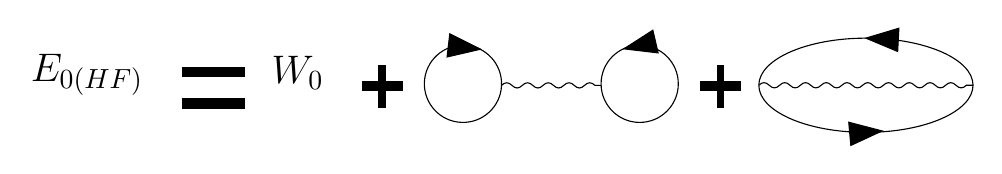
\begin{tikzpicture}[x=0.75pt,y=0.75pt,yscale=-1,xscale=1]
%uncomment if require: \path (0,244); %set diagram left start at 0, and has height of 244

%Shape: Circle [id:dp6498223397318404] 
\draw   (302,124.6) .. controls (302,114.33) and (310.33,106) .. (320.6,106) .. controls (330.87,106) and (339.2,114.33) .. (339.2,124.6) .. controls (339.2,134.87) and (330.87,143.2) .. (320.6,143.2) .. controls (310.33,143.2) and (302,134.87) .. (302,124.6) -- cycle ;
%Shape: Triangle [id:dp3898756772562222] 
\draw  [fill={rgb, 255:red, 0; green, 0; blue, 0 }  ,fill opacity=1 ] (313,107.75) -- (326.94,98.79) -- (329.46,109.7) -- cycle ;
%Shape: Cross [id:dp06220635309920053] 
\draw  [fill={rgb, 255:red, 0; green, 0; blue, 0 }  ,fill opacity=1 ] (195.01,115.6) -- (198.19,115.6) -- (198.19,123.61) -- (206.2,123.61) -- (206.2,127.99) -- (198.19,127.99) -- (198.19,136) -- (195.01,136) -- (195.01,127.99) -- (187,127.99) -- (187,123.61) -- (195.01,123.61) -- cycle ;
%Shape: Circle [id:dp6991360552110061] 
\draw   (216.87,123.85) .. controls (217.28,113.58) and (225.94,105.6) .. (236.2,106.01) .. controls (246.47,106.43) and (254.45,115.08) .. (254.04,125.35) .. controls (253.63,135.61) and (244.97,143.6) .. (234.71,143.18) .. controls (224.44,142.77) and (216.46,134.11) .. (216.87,123.85) -- cycle ;
%Shape: Triangle [id:dp7130261056413152] 
\draw  [fill={rgb, 255:red, 0; green, 0; blue, 0 }  ,fill opacity=1 ] (243.95,107.93) -- (227.8,111.66) -- (229.11,100.54) -- cycle ;
%Straight Lines [id:da10547511660578635] 
\draw    (254.04,125.35) .. controls (255.71,123.68) and (257.37,123.68) .. (259.04,125.35) .. controls (260.71,127.02) and (262.37,127.02) .. (264.04,125.35) .. controls (265.71,123.68) and (267.37,123.68) .. (269.04,125.35) .. controls (270.71,127.02) and (272.37,127.02) .. (274.04,125.35) .. controls (275.71,123.68) and (277.37,123.68) .. (279.04,125.35) .. controls (280.71,127.02) and (282.37,127.02) .. (284.04,125.35) .. controls (285.71,123.68) and (287.37,123.68) .. (289.04,125.35) .. controls (290.71,127.02) and (292.37,127.02) .. (294.04,125.35) .. controls (295.71,123.68) and (297.37,123.68) .. (299.04,125.35) -- (302,125.35) -- (302,125.35) ;
%Shape: Ellipse [id:dp18198799795452325] 
\draw   (378,125.3) .. controls (378,112.76) and (401.1,102.6) .. (429.6,102.6) .. controls (458.1,102.6) and (481.2,112.76) .. (481.2,125.3) .. controls (481.2,137.84) and (458.1,148) .. (429.6,148) .. controls (401.1,148) and (378,137.84) .. (378,125.3) -- cycle ;
%Shape: Triangle [id:dp6530702261537764] 
\draw  [fill={rgb, 255:red, 0; green, 0; blue, 0 }  ,fill opacity=1 ] (429.6,102.6) -- (445.47,97.82) -- (444.89,109.01) -- cycle ;
%Shape: Triangle [id:dp7883771420902802] 
\draw  [fill={rgb, 255:red, 0; green, 0; blue, 0 }  ,fill opacity=1 ] (437.37,147.3) -- (422.33,154.28) -- (421.33,143.12) -- cycle ;
%Straight Lines [id:da8945451528371555] 
\draw    (378,125.3) .. controls (379.67,123.63) and (381.33,123.63) .. (383,125.3) .. controls (384.67,126.97) and (386.33,126.97) .. (388,125.3) .. controls (389.67,123.63) and (391.33,123.63) .. (393,125.3) .. controls (394.67,126.97) and (396.33,126.97) .. (398,125.3) .. controls (399.67,123.63) and (401.33,123.63) .. (403,125.3) .. controls (404.67,126.97) and (406.33,126.97) .. (408,125.3) .. controls (409.67,123.63) and (411.33,123.63) .. (413,125.3) .. controls (414.67,126.97) and (416.33,126.97) .. (418,125.3) .. controls (419.67,123.63) and (421.33,123.63) .. (423,125.3) .. controls (424.67,126.97) and (426.33,126.97) .. (428,125.3) .. controls (429.67,123.63) and (431.33,123.63) .. (433,125.3) .. controls (434.67,126.97) and (436.33,126.97) .. (438,125.3) .. controls (439.67,123.63) and (441.33,123.63) .. (443,125.3) .. controls (444.67,126.97) and (446.33,126.97) .. (448,125.3) .. controls (449.67,123.63) and (451.33,123.63) .. (453,125.3) .. controls (454.67,126.97) and (456.33,126.97) .. (458,125.3) .. controls (459.67,123.63) and (461.33,123.63) .. (463,125.3) .. controls (464.67,126.97) and (466.33,126.97) .. (468,125.3) .. controls (469.67,123.63) and (471.33,123.63) .. (473,125.3) .. controls (474.67,126.97) and (476.33,126.97) .. (478,125.3) -- (481.2,125.3) -- (481.2,125.3) ;
%Shape: Cross [id:dp5950770882977249] 
\draw  [fill={rgb, 255:red, 0; green, 0; blue, 0 }  ,fill opacity=1 ] (358.01,115.6) -- (361.19,115.6) -- (361.19,123.61) -- (369.2,123.61) -- (369.2,127.99) -- (361.19,127.99) -- (361.19,136) -- (358.01,136) -- (358.01,127.99) -- (350,127.99) -- (350,123.61) -- (358.01,123.61) -- cycle ;
%Straight Lines [id:da7229955775391892] 
\draw [line width=3.75]    (100,119) -- (130.2,119) ;
%Straight Lines [id:da17096551384597625] 
\draw [line width=3.75]    (100,134) -- (130.2,134) ;

% Text Node
\draw (142,110) node [anchor=north west][inner sep=0.75pt]  [font=\Large]  {$W_{0}$};
% Text Node
\draw (26,109) node [anchor=north west][inner sep=0.75pt]  [font=\Large]  {$E_{0( HF)}$};


\end{tikzpicture}
\end{equation}
These diagrams involve only three simple rules, so we will evaluate them bere. The rules are: (1) $V_{klmn}$ for each interaction,(2) factor (-1) for each hole line and each fermion loop, and (3) a factor of $\frac{1}{2}$ because the graphs are symmetric. Remembering that all lines are hole lines here, we find
$$E_{0(H F)}=\sum_{k<k_{F}} \epsilon_{k}+\frac{1}{2} \sum_{k, l<k_{F}} V_{k l k l}-\frac{1}{2} \sum_{k ,l<k_{F}} V_{l k k l}$$
The approximation which is good for the high density electron gas (random phase approximation, or 'RPA') involves a partial sum over all 'ring' diagrams in second and higher order:
\begin{equation}
    \includegraphics[width=0.8\textwidth]{screenshots/many-body-vacuum-RPA-series.PNG}
\end{equation}
In the case of nuclear matter, we have the 'ladder approximation' involving a partial sum over all ladders:
\begin{equation}
    \includegraphics[width=0.8\textwidth]{screenshots/many-body-vacuum-ladder-series.PNG}
\end{equation}
\newpage
\section{Bird's-Eye View of Diagram Methods in the
Many-Body Problem}
\begin{table}[H]
        \centering
        
\begin{tabular}{p{0.45\textwidth}p{0.45\textwidth}}
\hline 
 \begin{center}
Field theoretic ingredient
\end{center}
 & \begin{center}
Significance in many-body theory
\end{center}
 \\
\hline 
 \begin{center}
(1)Occupation number notation
\end{center}
 & \begin{center}
Expresses arbitrary state of manybody system
\end{center}
 \\
\begin{center}
(2)Creation and destruction operators
\end{center}
 & \begin{center}
Primitive operators out of which all many-body operators are built
\end{center}
 \\
\begin{center}
(3)Single particle propagator (Green's function)
\end{center}
 & \begin{center}
Yields quasi particle energies, particle momentum distribution, particle density, ground energy
\end{center}
 \\
\begin{center}
(4)Vacuum amplitude
\end{center}
 & \begin{center}
Gives ground state energy
\end{center}
 \\
\begin{center}
(5)Two-particle Green's function propagator 
\end{center}
 & \begin{center}
Yields energies of collective excitations, electrical conductivity, other non-equilibrium properties
\end{center}
 \\
\begin{center}
(6)Finite temperature vacuum amplitude
\end{center}
 & \begin{center}
Gives equilibrium thermodynamic properties of system
\end{center}
 \\
\begin{center}
(7)Finite temperature propagator
\end{center}
 & \begin{center}
Yields temperature dependence of properties in (3)
\end{center}
 \\
\hline
\end{tabular}
        
\end{table}
\newpage
\section{Occupation Number Formalism (Second Quantization)}
\subsection{Advantages of occupation number formalism}
Since simple things can sometimes get to look pretty formidable in second quantization it is a good idea to understand why many-body physicists all use it. \bluep{The first reason is that it enables us to deal with systems containing a \textbf{variable number of particles}}.It turns out to give an enormous flexibility in the formalism if \textbf{N is allowed to vary in intermediate stages of a calculation and becomes fixed only at the end.} For example, we can put in and remove test particles at will, as in the case of the propagator. Or we can introduce the particle-hole formalism in which the number of particles and holes is variable.

The second reason for the occupation number formalism has to do with the symmetry properties of Fermi and Boss system. Doing things the old
way, we always have to worry about the complicated business of keeping the wave function properly symmetrized. But it turns out that in second quantization, the \textbf{creation and destruction operators obey certain commutation rules which have built into them all the symmetry properties of the system}. By just using these rules we are automatically free from symmetrization headaches.

\subsection{Many-body wave function in occupation number formalism}
Imagine that we are given a system of N identical fermions, which are in general interacting with each other and with an external potential. We have seen that such a system may be described in terms of a set of basis states, $|n_1,...,n_l,...\rangle$ in which the $n_l$ meant $n_l$ particles in the unperturbed single-particle energy eigenstate, $\phi_l$. Actually, \redp{the single-particle states used can be any orthonormal set}. This means that in general, $|n_1,...,n_l,...\rangle$ are not energy eigenstates of either the interacting or the non-interacting system of particles and their choice is determined by convenience. Foe the moment, we will use the $\phi$'s which satisfy the Schrodinger equation:
\begin{equation}\begin{aligned}
H \phi_{k \sigma}(\mathbf{r}, \gamma) &=\epsilon_{k o} \phi_{k o}(\mathbf{r}, \gamma) \\
H=\frac{p^{2}}{2 m}+U(\mathbf{r}) &=-\frac{1}{2 m} \nabla^{2}+U(\mathbf{r}) \\
(\hbar&=1)
\end{aligned}\end{equation}
and $\gamma, \sigma$ are the spin co-ordinate and quantum number respectively. In the case $U(\mathbf{r})=0,$ this has the solutions:
\begin{equation}\begin{aligned}
\phi_{k \sigma}(\mathbf{r}, \gamma) &=\frac{1}{\sqrt{\Omega}} e^{+i \mathbf{k} \cdot \mathbf{r}} \eta_{\sigma}(\gamma) \\
\epsilon_{k} &=\frac{k^{2}}{2 m}(\hbar=1)
\end{aligned}\end{equation}
where $\eta$ is the spin eigenfunction. In general, $\sigma, \gamma$ will be suppressed for brevity, and $\mathbf{k}$ will be short for $\mathbf{k}, \sigma,$ and $\mathbf{r} \equiv \mathbf{r}, \gamma$. 

If there are now N identical non-interacting fermions, the Hamiltonian and Schrodinger equation become
\begin{equation}\begin{array}{c}
H_{0}=\sum_{l=1}^{N} H_{l}, \quad H_{0} \Phi\left(\mathrm{r}_{1}, \ldots, \mathrm{r}_{N}\right)=E \Phi\left(\mathrm{r}_{1}, \ldots, \mathrm{r}_{N}\right) \\
H_{i}=\frac{p^{2}}{2 m}+U\left(\mathrm{r}_{i}\right) ; \quad H_{i} \phi_{k_{i}}=\epsilon_{k_{i}} \phi_{k_{i}}
\end{array}\end{equation}
since the system consists of identical fermions, the wave function must be antisymmetric, i.e., change sign when any two particle co-ordinates are interchanged. This is accomplished by forming a $\Phi$ given by the Slater determinant.
\begin{equation}\Phi_{k_{1} \ldots \ldots k_{N}}\left(\mathrm{r}_{1}, \ldots, \mathrm{r}_{N}\right)=\frac{1}{(N !)^{\frac{1}{2}}} \sum_{P} \gamma_{P} P\left[\phi_{k_{1}}\left(\mathrm{r}_{1}\right) \phi_{k_{2}}\left(\mathrm{r}_{2}\right) \ldots \phi_{k_{N}}\left(\mathrm{r}_{N}\right)\right]\end{equation}
or
\begin{equation}\Phi_{k_{1}, \ldots, k_{N}}\left(\mathbf{r}_{1}, \ldots, \mathbf{r}_{N}\right)=\frac{1}{(N !)^{\frac{1}{2}}}\left|\begin{array}{c}
\phi_{k_{1}}\left(\mathbf{r}_{1}\right) \phi_{k_{1}}\left(\mathbf{r}_{2}\right) \ldots \phi_{k_{1}}\left(\mathbf{r}_{N}\right) \\
\vdots \\
\phi_{k_{N}}\left(\mathbf{r}_{1}\right) \phi_{k_{N}}\left(\mathbf{r}_{2}\right) \dots \phi_{k_{N}}\left(\mathbf{r}_{N}\right)
\end{array}\right|
\label{slater-determinant-2}
\end{equation}
In the first form, $P$ is the permutation operator which interchanges the $\mathbf{r}_{i}$ 's in all possible ways (starting from some standard order), and $\gamma_{P}=-1$ for an odd number of interchanges, and +1 for an even number. The fact that $\Phi=0$ when any two $k_{i}$ 's are equal means that there can't be more than one particle in any state.

A tricky thing about (\ref{slater-determinant-2}) is its sign. For example, in a two-particle system with one particle in state $\phi_{1}$, and the other in $\phi_3$, the wave function is $\Phi_{k_1=1,k_2=3}\equiv\Phi_{13}$ or $\Phi_{k_1=3,k_2=1}\equiv\Phi_{31}$. Since the particles are identical, these represent the same state, but by (\ref{slater-determinant-2}) they differ by a minus sign. To remove this ambiguity, we always write $\Phi$ with the $k$'s in standard order given by:
\begin{equation}\Phi_{k_{1}<k_{2}<\ldots<k_{N}}\end{equation}
A compact way of writing $\Phi$ is
\begin{equation}\begin{aligned}
\Phi_{k_{1}, k_{2}, \ldots, k_{N}}\left(\mathbf{r}_{1}, \mathbf{r}_{2}, \ldots, \mathbf{r}_{N}\right) &=\Phi_{n_{1}, \ldots, n_{i}, \ldots}\left(\mathbf{r}_{1}, \mathbf{r}_{2}, \ldots, \mathbf{r}_{N}\right) \\
&=\left\langle\mathbf{r}_{1}, \mathbf{r}_{2}, \dots, \mathbf{r}_{N} | n_{1}, \dots, n_{i}, \dots\right\rangle
\end{aligned}\end{equation}
It is important to remember that \redp{the $\left|n_{1}, \ldots, n_{1}, \ldots\right\rangle$ are orthogonal and normal because the $\Phi_{k_{1}, \ldots, k_{N}}$ are}, and we may write this in the various equivalent ways
\begin{equation}\begin{array}{l}
\begin{aligned}
&\left\langle n_{1}^{\prime}, n_{2}^{\prime}, \ldots, n_{1}^{\prime}, \ldots | n_{1}, n_{2}, \ldots, n_{1}, \ldots\right\rangle  \\
& \equiv\left(\Phi_{n_{1}^{\prime}, n_{2}^{\prime}\ldots, n_{l}^{\prime}, \ldots} , \Phi_{n_{1}, n_{2}, \ldots, n_{l}, \ldots}\right) \\
& \equiv \int d^{3} \mathbf{r}_{1} \ldots d^{3} \mathbf{r}_{N} \Phi_{n_{1}^{\prime}, n_{2}}^{\prime}, \ldots .\left(\mathbf{r}_{1}, \ldots, \mathbf{r}_{N}\right) \Phi_{n_{1}, n_{2}, \ldots}\left(\mathbf{r}_{1}, \ldots, \mathbf{r}_{N}\right) \\
&=\delta_{n_{1}^{\prime}, n_{1}} \delta_{n_{2}^{\prime}, n_{2}} \ldots \delta_{n_{l}^{\prime}, n_{l}} \cdots .
\end{aligned}
\end{array}\end{equation}
Now we take the step to allow $N$ to be variable, running from 0 to $\infty$. Thus generates the set of basis functions in the following table:
\begin{table}[H]
\caption{Complete set of basis functions used in second quantization}
\centering
\begin{tabular}{ccc}
\hline
N        & $\Phi_{k_1,k_2,...k_N}$                   & $=|n_1,n_2,\ldots,n_i,\ldots\rangle$                                     \\ \hline
0        & $\Phi_0$                                  & $|000\ldots\rangle$                                                      \\
1        & $\Phi_{1}, \Phi_{2}, \Phi_{3}, \ldots$    & $|100 \ldots\rangle,|0100 \ldots\rangle,|00100 \ldots\rangle \ldots$     \\
2        & $\Phi_{12}, \Phi_{13}, \Phi_{23}, \ldots$ & $|1100 \ldots\rangle,|101000 \ldots\rangle,|01100 \ldots\rangle, \ldots$ \\
$\vdots$ & $\vdots$                                  & $\vdots$                                                                
\end{tabular}
\end{table}
This Hilbert space may be pictured as follows:
\begin{equation}
    \includegraphics[width=0.8\textwidth]{screenshots/extended-hilbert-space.PNG}
\label{extended-hilbert-space}
\end{equation}

This set is often called 'occupation number basis', and the whole formalism is sometimes referred to as '\redp{occupation number representation}'. Note carefully that we did not get this new basis by unitary transformation (like, for example, is done in going from position to momentum basis).

Only systems of independent fermions without perturbing interactions of any sort have been considered thus far. In the presence of such interactions, \bluep{the $\left.| n_{1}, \ldots, n_{t}, \ldots\right)$ are no longer eigenstates of the total Hamiltonian for the system and the correct eigenstates must be obtained as the linear combination}
\begin{equation}\begin{aligned}
\Psi^{\prime} &=\Phi_{0}+\sum_{k_{1}} A_{k_{1}} \Phi_{k_{1}}+\sum_{k_{1}<k_{2}} A_{k_{1}, k_{2}} \Phi_{k_{1}, k_{2}}+\cdots \\
&=\sum_{n_{1}, \ldots, n_{i}, \ldots} A_{n_{1}, \ldots, n_{i}, \ldots}\left|n_{1}, \ldots, n_{i}, \ldots\right\rangle
\end{aligned}\end{equation}

\subsection{Operators in occupation number formalism}
It was pointed out in Chapter 4 that all operators in this new formalism may be expressed in terms of the creation and destruction operator $c_i^{\dagger}$,$c_i$. The definition of these operators must include a factor of $(\pm1)$ because of antisymmetry. Thus, if $c_i^{\dagger}$,$c_i$ act in such a sequence on the wave function that their net efferct is to exchange two particles, then the wave function must change its sign. Some thought shows that the proper definition is 
\begin{equation}\begin{array}{l}
c_{1}^{\dagger}\left|n_{1}, \ldots, n_{1}, \ldots\right\rangle=(-1)^{\Sigma_{i}}\left(1-n_{i}\right)\left|n_{1}, \ldots, n_{i}+1, \ldots\right\rangle \\
c_{1}\left|n_{1}, \ldots, n_{1}, \ldots\right\rangle=(-1)^{\Sigma_{i}} n_{i}\left|n_{1}, \ldots, n_{i}-1, \ldots\right\rangle
\end{array}\end{equation}
where $\Sigma_i=n_1+n_2+\ldots n_{i-1}$. That is, we get a factor of (-1) for each particle (i.e., each occupied state) standing to the left of the state i in the wave function.

One of the nice properties of the $c_{1}^{\dagger}$ operators is that by applying them repeatedly to the "true vacuum" state (state with no particles in it), it is possible to generate all other states, thus:
\begin{equation}\begin{array}{l}
\Phi_{k_{1}, k_{2}, \ldots, k_{N}}=c_{k_{1}}^{\dagger} c_{k_{2}}^{\dagger} \ldots c_{k_{n}}^{\dagger}|000 \ldots\rangle \\
\left|n_{1}, n_{2}, \ldots\right\rangle=\left(c_{1}\right)^{n_{1}}\left(c_{2}\right)^{n_{2}} \ldots|0000 \ldots\rangle
\end{array}\end{equation}
Another important property of the $c_{1}^{\dagger}, c_{l}$ operators is that they are \redp{\textbf{'hermitian adjoints'}} of each other. This can be seen by constructing matrices for them, using the $\left|n_{1} n_{2}, \ldots, n_{1}, \ldots\right\rangle$ 's as basis states
\begin{equation}
    \begin{aligned}
    &\includegraphics[width=0.8\textwidth]{screenshots/hermitian-adjoint-1.PNG}\\
    &\includegraphics[width=0.8\textwidth]{screenshots/hermitian-adjoint-2.PNG}
    \end{aligned}
\end{equation}
so that
\begin{equation}c_{i}^{\dagger}=\left(c_{i}\right)^{\dagger}\end{equation}
\redp{\textbf{where $\dagger$ means hermitian adjoint. This further shows that $c_{h}^{\dagger} c_{l}$ are nonhermitian and are therefore not observables.}} (otherwise, we should have $c_i=c^{\dagger}_i$). Using the matrices above we can show that:
\begin{equation}\left(c_{i}^{\dagger} c_{i}\right)^{\dagger}=c_{i}^{\dagger} c_{i}\end{equation}
so that $c_i^{\dagger}c_i$ is hermitian. This combination is the famous "\textbf{\redp{number operator}}":
\begin{equation}\hat{n}_{l}=c_{l}^{\dagger} c_{l} ; \quad\left(\hat{N}=\sum_{l} c_{l}^{\dagger} c_{l}\right)\end{equation}
For example
$$c_{i}^{\dagger} c_{i}\left|n_{1}, \dots, n_{i}, \dots\right\rangle=n_{i}\left|n_{1}, \dots, n_{i}, \dots\right\rangle$$

\begin{imp}
The $c_{1}^{\dagger}, c_{1}$ operators obey the following important 'fermion commutation rules':
\begin{equation}
\begin{aligned}
&(1)\left[c_{l}, c_{k}\right]_{+}=c_{l} c_{k}^{\dagger}+c_{k}^{\dagger} c_{l}=\delta_{l k}\\
&(2)\left[c_{l}, c_{k}\right]_{+}=0\\
&(3)\left[c_{l}^{\dagger}, c_{k}^{\dagger}\right]_{+}=0
\end{aligned}
\label{anti-cmmutation-rules-c}
\end{equation}
\end{imp}
These can be easily proved from the definitions:
$$\begin{aligned}
c_{1} c_{k}\left|n_{1}, \ldots, n_{1}, \ldots, n_{k}, \ldots\right\rangle &=(-1)^{\Sigma_{x}} n_{k} c_{l}\left|n_{1}, \ldots, n_{l}, \ldots, n_{k}-1, \ldots\right\rangle \\
&=(-1)^{\sum_{k}+\Sigma_{l}} n_{k} n_{l}\left|n_{1}, \ldots, n_{l}-1, \ldots, n_{k}-1, \ldots\right\rangle
\end{aligned}$$
$$\begin{aligned}
c_{k} c_{l}\left|n_{1}, \ldots, n_{l}, \ldots, n_{k}, \ldots\right\rangle &=(-1)^{\Sigma_{l}} n_{l} c_{k}\left|n_{1}, \ldots, n_{l}-1, \ldots, n_{k}, \ldots\right\rangle \\
&=(-1)(-1)^{\Sigma_{k}+\Sigma_{l}} n_{k} n_{l}\left|n_{1}, \ldots, n_{l}-1, \ldots, n_{k}-1, \ldots\right\rangle
\end{aligned}$$
where the extra (-1) on line four comes from the fact that there is one less particle to the left of state k. Adding the two equations yields the second rule in (\ref{anti-cmmutation-rules-c}).

The importance of the above sets of' anti-commutation' relations lies in the fact that all the antisymmetry properties are built into them. Therefore, by using them in the right places, we don't have to worry either about the symmetry of the wave functions themselves.

\textbf{\redp{Let us now consider how to express the usual quantum operators in terms of $c_i^{\dagger}$,$c_i$.}} \textbf{We require equality between the matrix elements of the operator as computed in occupation number formalism and in the old cave-man formalism. For example, in a one-particle system, the operator $\mathcal{O}(\mathbf{r,p})$ with matrix elements:}
\begin{equation}O_{ij}=\left\langle\phi_{1}|\mathcal{O}| \phi_{j}\right\rangle=\int \phi_{i}^{*}(\mathbf{r}) \mathcal{O}(\mathbf{r}, \mathbf{p}) \phi_{j}(\mathbf{r}) d^{3} \mathbf{r}\end{equation}
has the occupation number form
\begin{equation}\mathcal{O}^{\mathrm{occ}}=\sum_{\boldsymbol{k}, l} \mathcal{O}_{k l} c_{k}^{\dagger} c_{l}\end{equation}
This is easily checked as
\begin{equation}\begin{aligned}
\left\langle 00 \ldots 1_{i} \ldots\left|\theta^{occ}\right| 00 \ldots 1_{j} \ldots\right\rangle &=\sum_{k, l} \mathcal{O}_{k l}\left\langle 00 \ldots 1_{i} \ldots\left|c_{k}^{\dagger} c_{l}\right| 00 \ldots 1_{j} \ldots\right\rangle \\
&=\sum_{k, l} \mathcal{O}_{k l} \delta_{lj} \delta_{i k}\\
&=\mathcal{O}_{ij}
\end{aligned}\end{equation}
Suppose we have an operator
\begin{equation}\mathcal{O}=\sum_{i=1}^{N} \mathcal{O}\left(\mathbf{r}_{i}, \mathbf{p}_{i}\right)\end{equation}
like for example the external potential:
\begin{equation}V\left(\mathbf{r}_{1}, \dots, \mathbf{r}_{N}\right)=\sum_{i=1}^{N} V\left(\mathbf{r}_{i}\right)\end{equation}
Such operators are called \redp{"one-body"} operators sicne they are a sum of operators each of which acts separately on one particle. Thus we have the valuable result that \textbf{\redp{in occupation number formalism, the single-particle operators have a form independent of N.}}

In a similar way, it can be shown that the "two-body" operator
\begin{equation}\mathcal{O}=\frac{1}{2} \sum_{\substack{i, j=1\\(i \neq j)}}^{N} \mathcal{O}\left(\mathbf{r}_{l}, \mathbf{p}_{i}, \mathbf{r}_{j}, \mathbf{p}_{j}\right)\end{equation}
For instance the interaction potential
\begin{equation}V\left(\mathbf{r}_{1}, \dots, \mathbf{r}_{N}\right)=\frac{1}{2} \sum_{\substack{i, j=1\\ (i \neq j)}} V\left(\mathbf{r}_{i}-\mathbf{r}_{j}\right)\end{equation}
becomes
\begin{equation}\mathcal{O}^{\mathrm{occ}}=\frac{1}{2} \sum_{k l m n} \mathcal{O}_{k \operatorname{lm} n} c_{l}^{\dagger} c_{k}^{\dagger} c_{m} c_{n}\end{equation}
where
\begin{equation}\mathcal{O}_{klmn}=\int d^{3} \mathbf{r} \int d^{3} \mathbf{r}^{\prime} \phi_{k}^{*}(\mathbf{r}) \phi_{i}^{*}\left(\mathbf{r}^{\prime}\right) \mathcal{O}\left(\mathbf{r}, \mathbf{r}^{\prime} ; \mathbf{p}, \mathbf{p}^{\prime}\right) \phi_{m}(\mathbf{r}) \phi_{n}\left(\mathbf{r}^{\prime}\right)\end{equation}
We remark here that the results also hold true in the case of bosons.

\subsection{Hamiltonian and Schrodinger equation In occupation number formalism}
\end{document}